%!TEX TS-program = xelatex
%!TEX encoding = UTF-8 Unicode


%%%%%%%%%%%%%%%%%%%%%%%%%%%%%%%%%%%%%%%%%
% The Legrand Orange Book
% LaTeX Template
% Version 2.0 (9/2/15)
%
% This template has been downloaded from:
% http://www.LaTeXTemplates.com
% License:
% CC BY-NC-SA 3.0 (http://creativecommons.org/licenses/by-nc-sa/3.0/)
% Important note:
% Chapter heading images should have a 2:1 width:height ratio,
% e.g. 920px width and 460px height.
%%%%%%%%%%%%%%%%%%%%%%%%%%%%%%%%%%%%%%%%%

\documentclass[11pt,fleqn,twoside]{book}
\usepackage{ctex}
\usepackage{indentfirst}
\usepackage{zhlineskip}
% \setCJKmainfont[BoldFont={SimHei},ItalicFont={KaiTi}]{SimSun}
\usepackage{mathrsfs}
\usepackage{cancel}
\usepackage{mathrsfs}
% \usepackage{siunitx}
\usepackage{physics}
\usepackage{ulem}
%\usepackage[version=3]{mhchem}
% \usepackage{draftwatermark}
% \SetWatermarkText{\textsc{Draft Translation}}
% \SetWatermarkLightness{0.9}
% \SetWatermarkScale{0.4}
\usepackage{marginfix}
%\include{marginpar}
\input{structure}
\usepackage{xypic}

\makeatletter
\def\UrlBreaks{\do\A\do\B\do\C\do\D\do\E\do\F\do\G\do\H\do\I\do\J
\do\K\do\L\do\M\do\N\do\O\do\P\do\Q\do\R\do\S\do\T\do\U\do\V
\do\W\do\X\do\Y\do\Z\do\[\do\\\do\]\do\^\do\_\do\`\do\a\do\b
\do\c\do\d\do\e\do\f\do\g\do\h\do\i\do\j\do\k\do\l\do\m\do\n
\do\o\do\p\do\q\do\r\do\s\do\t\do\u\do\v\do\w\do\x\do\y\do\z
\do\.\do\@\do\\\do\/\do\!\do\_\do\|\do\;\do\>\do\]\do\)\do\,
\do\?\do\'\do+\do\=\do\#}

\newcommand\figcaption{\def\@captype{figure}\caption} \newcommand\tabcaption{\def\@captype{table}\caption}
\makeatother

\newcounter{mparcnt}[chapter]
\renewcommand\themparcnt{\small{$^{\arabic{mparcnt}}$}}
\newcommand\mpar[1]{\refstepcounter{mparcnt}{$^{\arabic{mparcnt}}$}\marginpar{\themparcnt\scriptsize#1}}

\newcommand\picmpar[1]{\marginpar{%
    \captionsetup{type=figure}
    #1}%
}


%\makeatletter
%\def\mpar#1{%
%  {\refstepcounter{mparcnt}{$^{\arabic{mparcnt}}$}\marginpar{\themparcnt\tiny#1}}%
%}
%\def\mpar@macro#1[#2]{%
%  {\refstepcounter{mparcnt}{$^{\arabic{mparcnt}}$}\marginnote[#2]{\themparcnt\tiny#1}}
%}
%\makeatother

%% 句号
\catcode`\。=\active
\let。=.

\begin{document}
\frontmatter
\allowdisplaybreaks

%----------------------------------------------------------------------------------------
%	TITLE PAGE
%----------------------------------------------------------------------------------------

\begingroup
\thispagestyle{empty}
\begin{tikzpicture}[remember picture,overlay]
\coordinate [below=12cm] (midpoint) at (current page.north);
\node at (current page.north west)
{\begin{tikzpicture}[remember picture,overlay]
\node[anchor=north west,inner sep=0pt] at (0,0) {\includegraphics[width=\paperwidth]{background}}; % Background image
\draw[anchor=north] (midpoint) node [fill=ocre!30!white,fill opacity=0.6,text opacity=1,inner sep=1cm]{\Huge\centering\bfseries\sffamily\parbox[c][][t]{\paperwidth}{\centering 基于对称性的现代物理学 \\[15pt] % Book title
{\Large 原著:Jakob Schwichtenberg \quad 翻译:超理汉化组}\\[20pt] % Subtitle
{\huge } % Author name
{\huge Translate Version: \today}
}};
\end{tikzpicture}};
\end{tikzpicture}
\vfill
\endgroup

%----------------------------------------------------------------------------------------
%	COPYRIGHT PAGE
%----------------------------------------------------------------------------------------

\newpage
~\vfill
\thispagestyle{empty}

\noindent 本文档由热心网友翻译制作,原著书名为:\emph{Physics from Symmetry},属Springer公司Undergraduate Lecture Notes in Physics(ULNP)丛书,ISBN 978-3-319-19200-0,DOI 10.1007/978-3-319-19201-7。
\\ {\bfseries 仅限教学科研使用,使用与传播应严格遵守相关法律规定。}\\\\\\

\noindent《中华人民共和国著作权法》第四节第二十二条:\\
在下列情况下使用作品,可以不经著作权人许可,不向其支付报酬,但应当指明作者姓名、作品名称,并且不得侵犯著作权人依照本法享有的其他权利:\\
\dots \\
(六)为学校课堂教学或者科学研究,翻译或者少量复制已经发表的作品,供教学或者科研人员使用,但不得出版发行;\\
\dots \\\\



\noindent \copyright\ Springer International Publishing Switzerland 2015 \\

\noindent \copyright\ 2016 Chaoli-Translating-Group(超理汉化组) \\ % Copyright notice

\noindent \textsc{Not Published}\\ % Publisher

%\noindent \textsc{https://github.com/laserroger/Physics-from-Symmetry/}\\ % URL

%\noindent Licensed under the Creative Commons Attribution-NonCommercial 3.0 Unported License (the ``License''). You may not use this file except in compliance with the License. You may obtain a copy of the License at \url{http://creativecommons.org/licenses/by-nc/3.0}. Unless required by applicable law or agreed to in writing, software distributed under the License is distributed on an \textsc{``as is'' basis, without warranties or conditions of any kind}, either express or implied. See the License for the specific language governing permissions and limitations under the License.\\ % License information

%\noindent \textit{First printing, March 2013} % Printing/edition date

%----------------------------------------------------------------------------------------
%	TABLE OF CONTENTS
%----------------------------------------------------------------------------------------
\chapterimage{chapter_head_1.pdf} % Chapter heading image


\pagestyle{empty} % No headers


\cleardoublepage % Forces the first chapter to start on an odd page so it's on the right

\pagestyle{fancy} % Print headers again

%----------------------------------------------------------------------------------------
%	PART
%----------------------------------------------------------------------------------------

\input{Preface}
%!TEX encoding = UTF-8 Unicode

\chapter*{Acknowledgments}
感谢所有帮我编写这本书的人. 我特别感激Fritz Waitz, 他的评论, 想法与纠正让本书质量大大改善. 我十分感谢Arne Becker 和Daniel Hilpert, 感谢他们无价的建议,意见与细致的校对. 感谢Robert Sadlier对我英文的帮助以及Jakob Karalus的解释.

我还想感谢与我有许多见解深刻的讨论的Marcel K$\ddot{o}$pke, 感谢Silvia Schwichtenberg和 Christian Nawroth 的支持.

最后, 我亏欠最多的是我的父母, 他们支持着我, 教导我知识高于一切.

如果发现文中的错误, 我非常希望你能够寄一封短邮件到 errors@jakobschwichtenberg.com. 勘误表的地址是\url{http://physicsfromsymmetry.com/errata}.


\cleardoublepage
\pdfbookmark[chapter]{\contentsname}{toc}
\tableofcontents % Print the table of contents itself

\mainmatter

%!TEX encoding = UTF-8 Unicode

\part{Foundations 基础}

\begin{partquote}

{\bfseries “真相总比你想的简单”}\marginpar{``The truth always turns out to be simpler than you thought.''}


\begin{flushright}
--- Richard P. Feynman\\
as quoted by\\
K. C. Cole. {\itshape Sympathetic Vibrations.}\marginpar{%
K. C. Cole.\\ {\itshape Sympathetic Vibrations.}
Bantam, reprint edition,\\10 1985.\\
ISBN 9780553342345%
}
\end{flushright}
    
\end{partquote}


%!TEX encoding = UTF-8 Unicode

%----------------------------------------------------------------------------------------
%	CHAPTER 1
%----------------------------------------------------------------------------------------

\chapterimage{chapter_head_1.pdf} % Chapter heading image

\chapter{Introduction 简介}\label{chap1}

\section{What we Cannot Derive 得不到的事情}

在我们开始讲我们能从对称性里面了解到什么之前,我们首先澄清一下我们需要在我们的理论中人为的加一些什么东西。首先,目前没有任何理论可以得到自然界的常数。这些常数需要从实验中提取出来,比如各种相互作用的耦合常数啊,基本粒子的质量啊这种的。

除了这些,我们还有一些东西解释不了:{\bf 数字$3$}。这不是术数的那种神秘主义的东西,而是我们不能解释所有的直接与数字$3$相联系的限制。比如:

\begin{itemize}
\item 对应三种标准模型描述的基本作用力有三种规范理论\mpar{如果你不理解这个简介中的某些名词,比如规范理论或者二重覆盖,不需要太过担心。本书将会详尽的解释,在这里提到只是为了完整性。}。这些力是由分别对应于对称群$U(1), SU(2)$和$SU(3)$的规范理论描述的。为什么没有对应$SU(4)$带来的基本作用力?没人知道!
\item 轻子有三代,夸克也有三代。为什么没有第四代?我们只能从实验\mpar{比如,现在宇宙中元素的丰度是依赖于代的数量的。更进一步,对撞机实验中有对此的很强的证据。(见Phys. Rev. Lett. 109, 241802)}中知道没有第四代。
\item 我们只在拉格朗日量里面包含$\Phi$的最低三阶$(\Phi^0, \Phi^1, \Phi^2)$,其中$\Phi$指代一些描述我们的物理系统的东西,是个通称,而这个拉格朗日量则是被我们用来得到我们的描述自由(=无相互作用)场/粒子的靠谱的理论的。
\item 我们只用三个基本的Poincare群双覆盖的表示,分别对应自旋$0, \tfrac{1}{2}$和$1$。没有基本粒子的自旋是$\tfrac{3}{2}$。
\end{itemize}

在现代的理论中,这些是我们必须手动增加的假定。我们从实验上知道这些假定是正确的,但是目前为止我们没有更深刻的原理告诉我们为什么我们需要到$3$就停。

除此之外,还有两件事情我们没法从对称性中得到,但是他们对于一个严谨的理论来说有时必须被考虑到的:

\begin{itemize}
\item 我们只允许在拉格朗日量中引入尽可能低阶的非平庸的微分算符$\partial_\mu$。对于一些理论,我们使用一阶的微分算符$\partial_\mu$,而另一些理论Lorentz不变形禁止了一阶导数,从而二阶导数$\partial_\mu\partial^\mu$是最低阶的可能的非平庸阶项。除此之外我们就再也得不到一个合理的理论了。存在高阶导数项的理论没有下界,这导致能量可以是一个任意大小的负值;因此,这些理论中的态总可以变到能量更低的态,从而永远不会稳定。
\item 我们处于类似的原因,我们可以说如果半整数自旋的粒子和整数自旋的粒子拥有完全一样的行为的话,宇宙中就不会有稳定的物质。因此,这两者必然有某些{\it 东西}不一样,而我们没得选,只有一种可能而且合理的选择\mpar{我们在最开始的量子场论里使用反对易子而不是对易子,从而防止我们的理论变成没有下界的理论。}是正确的。这引出了半整数自旋粒子的Fermi-Dirac统计的概念和整数自旋粒子的Bose-Einstein统计的概念。半整数自旋的粒子从而通常被称为Fermion,它们中永远不存在两个粒子处在完全一样的态上。而与之相反的,这种情况对整数自旋的粒子 -- 通常被称为Boson -- 是可能的。
\end{itemize}

最后呢,我们提一下剩下的一个我们不能从这本书的其他理论中得到的东西:{\bf 引力}。当然,实际上,大名鼎鼎的广义相对论就是优美而准确的描述引力的理论;然而这个理论与其他理论完全不一样,超出了本书的研究范围。而尝试将引力问题划入相同框架下的量子引力理论仍待完善:目前没有人能够成功得出它。除此之外,在最后一章我们会做一些对引力的一些评述。

\section{Book Overview 全书概览}

\begin{center}
  \makebox[\textwidth][c]{\quad\quad\quad\quad
\small\xymatrix{
& \underset{\overset{|}{\text{不可约表示}}}{\text{Poincare群的双覆盖}}\ar[d]  &\\
&\ar[dl]\ar[d]\ar[dr] &\\
(0,0): \text{自旋$0$表示}\ar[d]_{\text{作用}}^{\text{在}}&(\tfrac{1}{2},0)\oplus(0,\tfrac{1}{2}): \text{自旋$\tfrac{1}{2}$表示} \ar[d]_{\text{作用}}^{\text{在}}&(\tfrac{1}{2},\tfrac{1}{2}): \text{自旋$1$表示}\ar[d]_{\text{作用}}^{\text{在}}\\
\text{标量}\ar[d]_{\text{保证拉格朗日量}}^{\text{是(对称变换)不变的}}&\text{旋量} \ar[d]_{\text{保证拉格朗日量}}^{\text{是(对称变换)不变的}}&\text{矢量}\ar[d]_{\text{保证拉格朗日量}}^{\text{是(对称变换)不变的}}\\
\text{自由的自旋$0$体系的拉格朗日量}\ar[d]_{\text{欧拉-拉格朗}}^{\text{日方程}}&\text{自由的自旋$\tfrac{1}{2}$体系的拉格朗日量} \ar[d]_{\text{欧拉-拉格朗}}^{\text{日方程}}&\text{自由的自旋$1$体系的拉格朗日量}\ar[d]_{\text{欧拉-拉格朗}}^{\text{日方程}}\\
\text{Klien-Gordon方程}&\text{Dirac方程}&\text{Proka方程}
}}
\end{center}

这本书使用{\bf 自然单位制},也就是说Planck常数$\hbar = 1$,光速$c=1$。这是基本理论中使用的惯例,它免除了很多不必要的笔墨。而对于应用来说呢,这些常数需要被再一次的加上去从而回到标准的SI单位制。

{\bf 狭义相对论}的基本假设是我们的起始点;它们是:在所有的惯性参考系--一些相互之间的速度保持恒定的参考系--中,光的速度不变,为$c$;而且所有的惯性参考系中的物理是一样的。

满足这些对称性的所有的变换构成的集合叫做{\bf Poincare群}。






%!TEX root = ./../main.tex
%!TEX encoding = UTF-8 Unicode
%----------------------------------------------------------------------------------------
%   CHAPTER 2
%   translator: InSight
%   proofreader: SI
%----------------------------------------------------------------------------------------

\chapterimage{chapter_head_1.pdf} % Chapter heading image



\chapter[狭义相对论]{Special Relativity \quad 狭义相对论}
\label{chap2}
 著名的Michelson-Morley实验告诉我们,光在任何参考系中都具有相同的速度\mpar{日常生活中所观测到的物体的速度取决于选定的参考系。如果一个观察者站在火车站上,测得的火车速度为$50 \mathrm{km\,h^{-1}} $,另一个观察者以$15\mathrm{km\,h^{-1}}$ 的速度与火车一同运动,那么测得的火车速度就应是$35 \mathrm{km\,h^{-1}}$。与此不同的是,光始终以$1.08 \times 10^9 \mathrm{km\,h^{-1}}$运动,不论如何相对于光运动。}。Albert Einstein首先意识到这个结果所蕴含的深刻意义,从而在此基础之上建立了狭义相对论。从光速不变原理出发,Einstein预言了许多有趣而又悖于常理的现象,最后都被实验证实是正确的。在这里我们首先阐明狭义相对论的基础,然后再体会这个原理的强大之处。狭义相对论有两个基本假设:
 \begin{itemize}
   \item {\bf{相对性原理:}} 任意惯性系,即任意两个相对速度恒定的参考系的物理规律相同。
   \item {\bf{光速不变原理:}} 在任意惯性系中的光速均为常数$c$。
 \end{itemize}
除此之外,我们还假设时空均匀且各向同性。这意味着不论在哪儿(均匀),不论朝着什么方向(各向同性)做实验,物理规律都是一样的。例如两个物理学家,一个在纽约,一个在东京,他们做完全一样的两个实验,会得到相同
\mpar{这当然要排除某些参数的影响,例如重力加速度。}  的物理规律,就算是在火星也一样。

%翻译欠佳,主语应该换换
正确的物理定律不应该随看实验的角度%这里我不太确定
或是进行实验的时间点而变。\footnote{原文为:The laws of physics, formulated correctly, shouldn't change if you look at the experiment from a different perspective or repeat it tomorrow.}此外,狭义相对论的第一条假设告诉我们,不管是在匀速运动的马车上,还是是在静止的实验室中,做同一物理实验都会得到相同的结果。以上论述均与与我们的生活经验相符。举个例子,如果你闭着眼睛坐在匀速运动的汽车上,你是没有办法分辨出你是真的在运动还是静止的。

如果没有了各向同性和均匀性,物理学就会遇到很大的麻烦:从实验中得到的物理定律如果仅仅在空间中的某一点对于确定的某一方向成立,显然是毫无用处的。

唯一有些不直观的就是狭义相对论的第二条假设,毕竟它违背了我们所有的日常经验。虽然如此,至今为此所有的实验都表明这个假设是正确的。
\section[狭义相对论的中的不变量]{The Invariant of Special Relativity \quad 狭义相对论的中的不变量}
\label{sec2.1}
在接下来的几节中,我们将使用狭义相对论的两个基本假设推导出Minkowski度规,有了它,我们就能计算两个物理事件的“距离”。物理事件在这里指在Minkowski 时空中的点,而整个狭义相对论都建立在Minkowski时空之上。我们从而得知任意两个不同惯性参考系之间的变换必须保证Minkowski度规不变,通过这一条件我们能够找到连接两个允许存在的惯性系(也就是光速为常数的参考系)之间所有的变换\footnote{非常类似我们要找旋转变换对应的各个参数的变换规律,而旋转变换保证了长度的守恒}。
在本书其余的部分我们将会用到这些关于变换的知识,来寻找在这些变换下不变的方程。让我们从一个能导出一条狭义相对论假设的最重要的推论之一的思想实验开始。
{\marginpar{
    \centering
    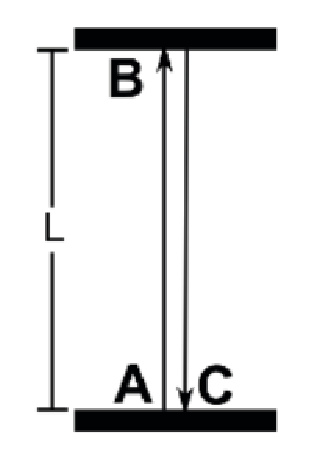
\includegraphics[scale=0.5]{fig2_1.eps}
    \figcaption{思想实验图示}
    \label{fig2.1}
}}
设想坐标系中一观察者,在原点处向上发出一个光脉冲,经过一段时间后被垂直镜面反射回原点。如图\ref{fig2.1}所示

有3个重要的事件:
\begin{itemize}
  \item {\bf{A:}}光从原点发出
  \item {\bf{B:}}光在镜面上反射
  \item {\bf{C:}}光回到原点
\end{itemize}
事件{\bf{AC}}之间的时间间隔为\mpar{对于恒定速度$v$而言,有$v=\frac{\Delta s}{\Delta t}$,$\Delta s$表示经过的距离,$\Delta t$代表所需时间,因此$\Delta t=\frac{\Delta s}{v}$}
\begin{equation}\label{equ2.1}
\Delta t=t_C-t_A=\frac{2L}{c}
\end{equation}
式中$L$表示原点与反射点之间的距离。

{\marginpar{
        \centering
        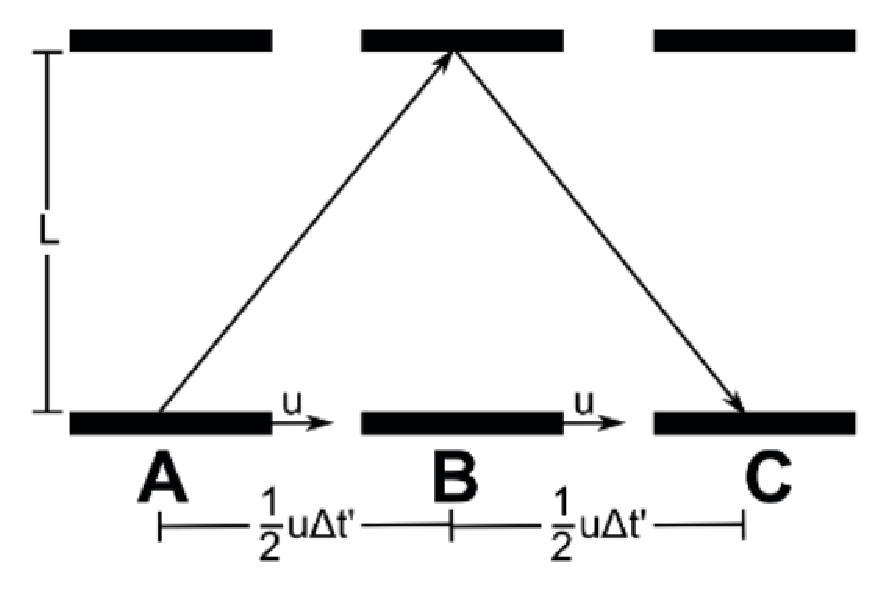
\includegraphics[scale=0.31]{fig2_2.eps}
        \figcaption{思想实验图示. 第二位移动观察者向左移动, 因此第一位观察者相对他向右移动}
        \label{fig2.2}
}}


接下来考虑第二位观察者,在$t_A$时刻处于他所在的坐标系的原点,并以恒定速度$u$相对于第一个观察者\mpar{那些能将两相对速度恒定的惯性参考系中的物理量相互转化的变换称为
{\bf{推动(Boost)}}变换, 后面我们会对此进行详述。}向左运动。为简便起见,我们假设第二个参考系的原点在$t_A$时刻与第一位观察者的坐标系原点重合。第二位观察者所见到的现象就与第一位不一样了。在他的参考系中,光脉冲的起点和终点并不在同一位置(见图\ref{fig2.2})。

用数学语言表示:
\begin{equation}\label{equ2.2}
  x'_A=0 \neq x'_C=u \Delta t' \qquad \rightarrow \qquad \Delta x' =u \Delta t'
\end{equation}
带撇物理量代表第二位观察者所测量的量。对于第一位静止系的观察者而言有
\begin{equation}\label{equ2.3}
  x_A=x_C \qquad \rightarrow \qquad \Delta x=0
\end{equation}
假定了第二位观察者运动沿$x$轴,因此
\begin{equation}\label{equ2.4}
 y'_A=y'_C \quad  \quad z'_A=z'_C \quad \rightarrow \quad \Delta y'=0 \quad  \quad \Delta z'=0
\end{equation}
那么同样也有
\begin{equation}\label{equ2.5}
 y_A=y_C \quad  \quad z_A=z_C \quad \rightarrow \quad \Delta y=0 \quad  \quad \Delta z=0
\end{equation}

接下来的问题是:{\bf{第二位观察者所测得的时间间隔是多少?}}因为已经假定了光速为常数,那么事件{\bf{AC}}对于第二位观察者而言将具有不同的间隔!时间间隔$\Delta t'=t'_C-t'_A$,等于光在第二位观察者的参考系中走过的距离$l$除以光速$c$。
\begin{equation}\label{equ2.6}
  \Delta t'=\frac{l}{c}
\end{equation}
我们可以利用古老的Pythagoras\footnote{通译为毕达哥拉斯。}定理(见图\ref{fig2.2}) 计算光传播的距离
\begin{equation}\label{equ2.7}
  l=2 \sqrt{\left(\frac{1}{2} u \Delta t'\right)^2+L^2}
\end{equation}
利用式\eqref{equ2.6}可以得到
\begin{equation}\label{equ2.8}
  c \Delta t' =2 \sqrt{\left(\frac{1}{2} u \Delta t'\right)^2+L^2}
\end{equation}
再利用式\eqref{equ2.2}中的$\Delta x'=u\Delta t'$可得
\begin{displaymath}
c \Delta t' =
  2 \sqrt{\left(\frac{1}{2} u \Delta t'\right)^2+L^2}
\end{displaymath}
\begin{displaymath}
  \rightarrow
  \left( c \Delta t' \right)^2 =
   4 \left( \left(\frac{1}{2} u \Delta t'\right)^2+L^2 \right)
\end{displaymath}
\begin{equation}\label{equ2.9}
\rightarrow
\left( c \Delta t' \right)^2
-\left(\Delta x' \right)^2=
4 \left( \left(\frac{1}{2} u \Delta t'\right)^2+L^2 \right)
-\left(\Delta x' \right)^2 =4L^2
\end{equation}
 现在回到式\eqref{equ2.1},即$\Delta t =\frac{2L}{c}$,那么
\begin{equation}\label{equ2.10}
 \left( c \Delta t' \right)^2
 -\left(\Delta x' \right)^2
 =4 L^2
 =\left( c \Delta t \right)^2
 =\left( c \Delta t \right)^2
 -
 \!\!\!
 \underbrace{\left(\Delta x \right)^2}_{=0 \text{由式}\eqref{equ2.3} \text{知}}
\end{equation}
终于,我们得到\mpar{\it{注意到我们在此处采用的是得到这个结果的最简方法,因为我们假定$t_A$时刻两坐标的原点是重合的。尽管如此,就算我们任意选择两惯性参考系原点的关系,仍然可以证明这个结论,只是过程会复杂一些。因为物理定律在任意惯性系中都是一样的,这给了我们任意选择便于计算的参考系的自由。如果第二位观察者的参考系运动方向是任意的,那就不再有$\Delta y'=0$和$\Delta z'=0$,但虽然如此,我们能够证明方程仍然是成立的,因为物理定律在任意惯性系中都是一样的。$^{\color{red}{4}}$\ \\ \ \\ {$^{\color{red}{4}}$ 译者注:原文的确把这句话说了两遍}}}

\begin{equation}\label{equ2.11}
\left( c \Delta t' \right)^2
-\left(\Delta x' \right)^2
-\underbrace{\left(\Delta y' \right)^2}_{=0}
-\underbrace{\left(\Delta z' \right)^2}_{=0}
=
\left( c \Delta t \right)^2
-\underbrace{\left(\Delta x \right)^2}_{=0}
-\underbrace{\left(\Delta y \right)^2}_{=0}
-\underbrace{\left(\Delta z \right)^2}_{=0}
\end{equation}
考虑第三个观察者,相对于第一个观察者以不同的速度运动,用同样的推理可以得到
\begin{equation}\label{equ2.12}
\left( c \Delta t'' \right)^2
-\left(\Delta x'' \right)^2
-\left(\Delta y'' \right)^2
-\left(\Delta z'' \right)^2
=
\left( c \Delta t \right)^2
-\left(\Delta x \right)^2
-\left(\Delta y \right)^2
-\left(\Delta z \right)^2
\end{equation}
因此,我们得到了一些对于所有观察者都相同的量:即二次型
\begin{equation}\label{equ2.13}
(\Delta s)^2
\equiv\left( c \Delta t \right)^2
-\left(\Delta x \right)^2
-\left(\Delta y \right)^2
-\left(\Delta z \right)^2
\end{equation}

此外,我们还能看出对于不同观察者,$(\Delta x)^2+(\Delta y)^2+(\Delta z)^2$或者说$(c\Delta t)^2$是不同的。我们将在下一节讨论不变量$\Delta s^2$所蕴含的物理意义。


\section[固有时]{Proper Time \quad 固有时}
\label{sec2.2}
我们在上一节推导出了狭义相对论中的不变量$\Delta s^2$,其在所有观察者眼中都相同。接下来我们要讨论这个量的物理意义。
    \marginpar{
        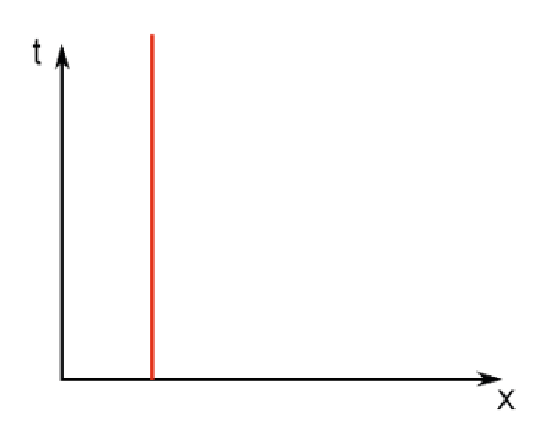
\includegraphics[scale=0.4]{fig2_3.eps}
        \figcaption{静止物体的世界线。物体位置不随时间流逝而变化。}\label{fig2.3}
    }
为简便起见,我们将问题限制在一维空间中。对于一个相对于观察者静止的物体,我们能作出它的时空图(见图\ref{fig2.3})。相应的,一个匀速运动的物体能作出如图\ref{fig2.4}所示的时空图。

    \marginpar{
        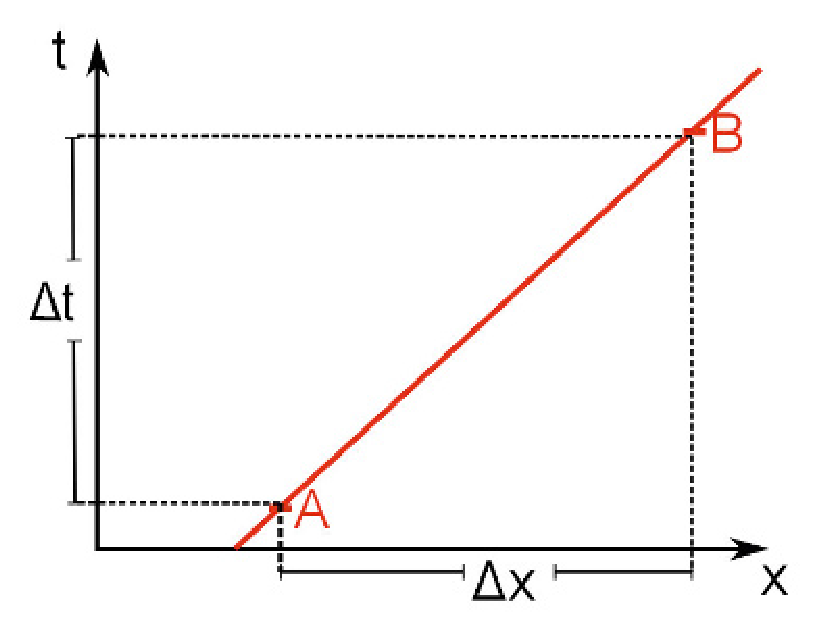
\includegraphics[scale=0.35]{fig2_4.eps}\label{fig2.4}
        \figcaption{某匀速直线运动物体的世界线。物体前后经过某两点记为事件A,B。它们间的空间距离为$\Delta x$,时间间隔为$\Delta t$}
    }
我们画来用于确定物体在时空中位置的线称为{\bf{世界线(world line)}}。世界线总是依赖于观察者的。两不同观察者对于同一物体可能会画出完全不同的世界线。若一观察者眼中的物体时空图为图\ref{fig2.4},那么对于速度与物体相同的观察者,其时空图将为图\ref{fig2.5},即对于此观察者物体静止。为了解释两位观察者给出的不同描述,我们引入$x'$ 和$t'$ 表示第二位观察者的参考系中的时间和位置。\footnote{注意:我们这里使用的例子与节\ref{sec2.1}不同}

我们可以看到,两个观察者将对事件$AB$之间的变化持不同观点。对于第一位观察者,$\Delta x \neq 0$, 但对于第二位观察者,$\Delta x' = 0$。 两观察者都认为事件$A$ 和$B$ 之间的时间间隔非零:$\Delta t \neq 0$ 和$\Delta t' \neq 0$,且认为$\Delta s^2$也相同(见上节推导的结论,任意观察者都有相同的$\Delta s^2$)。 这将导出一个令人惊讶的结论:事件$A$ 到$B$ 经历的时间对于两观察者不同
    \marginpar{
        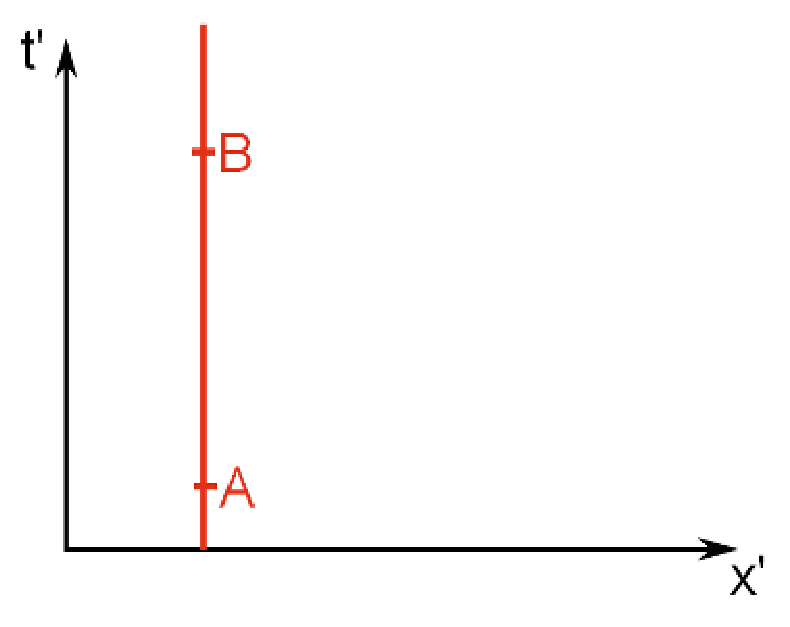
\includegraphics[scale=0.35]{fig2_5.eps}
        \figcaption{同一个运动物体的世界线,但观察者与该物体速度相同。该观察者观测到的事件AB之间的空间距离为$\Delta x' = 0$}\label{fig2.5}
    }
\begin{equation}\label{equ2.14}
  (\Delta s)^2
  =(c\Delta t)^2
  -(\Delta x)^2
\end{equation}
\begin{equation}\label{equ2.15}
  (\Delta s')^2
  =(c\Delta t')^2
  -\underbrace{(\Delta x')^2}_{=0}
  =(c\Delta t')^2
\end{equation}
\begin{equation}\label{equ2.16}
   (\Delta s)^2
   = (\Delta s')^2
   \rightarrow
    (\Delta t')^2 \neq
     (\Delta t')^2
     \quad \text{因为}  (\Delta x)^2 \neq 0
\end{equation}

这是有关狭义相对论最著名的一个效应,通常称为{\bf{钟慢效应(time-dilation)}}。时间间隔依赖于观察者,正如空间距离一样。不同观察者时间流逝速度不同,因此两事件经历的时间也就自然不同了。

现在时间将变为一个相对的概念,如果我们能找到一个对于所有观察者都相同的时间量,这将会非常有用。在上述例子中,第二位观察者与物体有相同的速度,有
\begin{equation}\label{equ2.17}
  (\Delta s')^2
  =(c\Delta t')^2
\end{equation}

上式意味着狭义相对论中的不变量恰为观察者所观测到的时间间隔乘上光速$c$。这让我们有机会能用$(\Delta s)^2$定义一个对于所有观察者相同的时间量。我们定义
\begin{equation}\label{equ2.18}
  (\Delta s)^2
  =(c\Delta \tau)^2
\end{equation}
$\tau$称为{\bf{固有时(proper time)}}。固有时是所有相对于该物体静止的观察者所测量的时间。

当然,现实生活中的物体绝非只能做匀速运动,但我们可以取足够短的时间(无穷小),使得运动近似为匀速运动,这样固有时的概念就说得通了。因此数学上我们需将概念过渡到无穷小,即$\Delta \rightarrow d$:
\begin{equation}\label{equ2.19}
  (ds)^2  =(cd \tau )^2=(cdt)^2-(dx)^2-(dy)^2-(dz)^2
\end{equation}

因此,就算一个物体到处乱跑,我们也能假设一个与物体一起运动的自带时钟的观察者,这样他总与该物体相对静止。对于这个特定的观察者而言,他所测量的时间间隔就是固有时,这一数值对其余观察者也是相同的,因为$(ds)^2=(cd\tau)^2$对于任意观察者成立。再次强调,这并不意味着对所有观察者都有同样的时间间隔,只是这些观察者承认该特殊观察者所测量的时间间隔为一不变量罢了。

\section[速度上限]{Upper Speed Limit \quad 速度上限}
\label{sec2.3}
在上节中我们对狭义相对论这一不变量有了解释,现在可以更进一步,导出另一个狭义相对论的惊人结论。

由于不变量的定义中带有负号,这意味着对于时空中的两个事件,$(\Delta s)^2$的值可能为0。$(\Delta s)^2$的值甚至可能是负的,但这样我们将得到一个复的固有时\mpar{按固有时定义,$(ds)^2=(cd\tau)^2$,$(ds)^2 < 0 \rightarrow d\tau$ 为复数。},通常复的固有时没有物理意义。因此,$(\Delta s)^2=0$时固有时最小,$\tau=0$,令
\[
\Delta s^2_{min}
=0=(c \Delta t)^2-(\Delta x)^2-(\Delta y)^2-(\Delta z)^2
\]
\[
\rightarrow (c \Delta t)^2
=(\Delta x)^2+(\Delta y)^2+(\Delta z)^2
\]
\begin{equation}\label{equ2.20}
 \rightarrow c^2=
  \frac{(\Delta x)^2+(\Delta y)^2+(\Delta z)^2}{(\Delta t)^2}
\end{equation}
在上式右侧我们有速度平方$v^2$,也就是距离除上时间,把这个式子写成极限,则
\begin{equation}\label{equ2.21}
 \rightarrow c^2=\frac{(d x)^2+(d y)^2+(d z)^2}{(dt)^2}
\end{equation}
函数$x(t)$,$y(t)$,$z(t)$是描述两事件之间路径的参数方程,这样式子右侧就是两事件间的运动速率。
%flag 此处的速度在文中并无主语,可能要加上物体二字,那么前面也得改。

因此,当某一观察者测得的固有时为$0$时其速度将满足下式
\begin{equation}\label{equ2.22}
  \rightarrow c^2 =v^2
\end{equation}
这意味着没有物体能以超过光速$c$的速度运动!\footnote{译者注:否则其固有时为复}{\bf{我们给物理学中的一切事物找到了一个速度上限。}}时空中的两事件相互影响的传播速度不能超光速。

{\it{这一点满足物理学上的{\bf{局域性原理(principle of locality)}},即物理学中的对象只能被它邻近的对象影响。相互作用都是局域的,不存在超距作用,物理效应的传播需要时间。}}

\section[Minkowski记法]{The Minkowski Notation \quad Minkowski 记法}
\label{sec2.4}
\begin{quote}
从现在起,孤立的空间和孤立的时间注定要消失成为影子,只有两者的统一才能保持独立的存在。
\end{quote}
\begin{flushright}
  {\bf{-Hermann Minkowski}}\mpar{出自Hermann Minkowski在Assembly of German Natural Scientists and Physicians(1908.9.21)上的演讲}
\end{flushright}
写出狭义相对论中不变量
\begin{equation}\label{equ2.23}
 ds^2=(cdt)^2-(dx)^2-(dy)^2-(dz)^2
\end{equation}
在此处将采用一种新的记法,这种记法初学时可能稍显复杂,不过后文中将经常用到:\\
\begin{align}
ds^2&=\eta^{\mu\nu}dx_\mu dx_\nu \notag \\
&=\eta^{00}(dx_0)^2+\eta^{11}(dx_1)^2+\eta^{22}(dx_2)^2+\eta^{33}(dx_3)^2 \notag \\
&=dx_0^2-dx_1^2-dx_2^2-dx_3^2\notag \\
&=(cdt)^2-(dx)^2-(dy)^2-(dz)^2 \label{equ2.24}
\end{align}
在这里我们用了一些新的约定和记号,这些东西在近代物理中应用很广泛,所以越早熟悉越好:
\begin{itemize}
  \item Einstein求和约定:某指标在同一项内出现两次则代表遍历该指标并求和。例如:$\sum_{i=1}^3a_i b_i =a_i b_i=a_1 b_1 +a_2 b_2 +a_3 b_3$,但$\sum_{i=1}^3a_i b_j=a_1 b_j +a_2 b_j +a_3 b_j\neq a_i b_j$
  \item 像$\mu$,$\nu$,$\sigma$这样的希腊字母
  \mpar{像 $i$,$j$,$k$这样的罗马字母作指标时一般代表从1到3求和:$x_i x_i \equiv \sum_i^3 x_i x_i$。 后面我们还会用到大写的罗马字母如$A$,$B$,$C$,它们作指标时代表从1到8求和。} 作指标时,一般代表从0 到3 求和:$x_\mu y_\mu=\sum_{\mu=0}^3 x_\mu y_\mu $
  \item 我们约定变量$x_0\equiv ct$,$x_1\equiv x$,$x_2\equiv y$,$x_3\equiv z$。这样时间空间地位等同,也便于我们使用Einstein求和约定
  \item 引入Minkowski度规($\eta$看作一矩阵,$\eta^{ij}$ 为其矩阵元):$\eta^{00}=1$,$\eta^{11}=-1$,$\eta^{22}=-1$,$\eta^{33}=-1$,当$\mu \neq \nu$时$\eta^{\mu\nu}=0$  (也可以等价的写为
\mpar{$\eta^{\mu\nu}= \\ \\
       \left(
       \begin{array}{cccc}
        1 & 0 & 0 & 0 \\
         0 & -1 & 0 & 0 \\
          0 & 0 & -1 & 0 \\
          0 & 0 & 0  & -1\\
        \end{array}
        \right)$ }
      $\eta^{\mu\nu} = \mathrm{diag} (1,-1,-1,-1)$)
\end{itemize}

另外按常规我们还要引入{\bf{四维矢量(four-vector)}},简称{\bf{4矢}}。
\begin{equation}\label{equ2.25}
  dx_\mu =\left(\begin{array}{c}
            dx_0 \\
            dx_1 \\
            dx_2 \\
            dx_3
          \end{array}\right)
\end{equation}
式\eqref{equ2.24}可用4矢和Minkowski度规表出
\begin{align}
  &(ds)^2=dx_\mu \eta^{\mu\nu} dx_\nu \notag \\
  &=\left(
     \begin{array}{cccc}
       dx_0 & dx_1 & dx_2 & dx_3 \\
     \end{array}
   \right)
   \!\!\!
   \left(
     \begin{array}{cccc}
       1 & 0 & 0 & 0 \\
       0 & -1 & 0 & 0 \\
        0 & 0 & -1 & 0 \\
        0 & 0 & 0  & -1\\
     \end{array}
   \right)
   \!\!\!
   \left(
     \begin{array}{c}
       dx_0 \\
        dx_1 \\
       dx_2 \\
        dx_3\\
     \end{array}
   \right)\notag \\
   &=dx_0^2-dx_1^2-dx_2^2-dx_3^2 \label{equ2.26}
\end{align}

采用这种记法能让我们省不少事。对于$ds$,我们给出的解释是时空(Minkowski时空)中两事件的“距离”,这个“距离”并不只是空间距离,它还将时间间隔考虑在内。如果我们考虑3维Euclidean 空间\mpar{3维Euclidean空间就是经典物理中一般的空间,在此空间中我们将时间和空间分别处理,也就是未将时空考虑成一个整体的几何结构来考虑。但一旦将时间作为新坐标,结合出时空的观念,我们便能将时间空间放在同一坐标下考虑。}中两点间最短距离的平方\mpar{Kronecker函数$\delta_{ij}$即是单位矩阵在指标记法下的表示,详见附录\ref{appendix.B.5.5}}
\begin{align}
  (ds)^2&=dx_i \delta^{ij} dx_j \notag \\
            &=\left(
               \begin{array}{ccc}
                dx_1 & dx_2 & dx_3 \\
               \end{array}
               \right)
               \left(
               \begin{array}{ccc}
                1 & 0 & 0  \\
                0 & 1 & 0  \\
                0 & 0 & 1  \\
              \end{array}
              \right)
              \left(
              \begin{array}{c}
               dx_1 \\
               dx_2 \\
               dx_3\\
              \end{array}
              \right)\notag \\
           &=(ds)^2=(dx_1)^2+(dx_2)^2+(dx_3)^2\label{equ2.27}
\end{align}

这种能够告诉我们无限临近的两点间的距离叫{\bf{度规(metric)}}。在Euclidean空间中度规就是单位矩阵$\delta_{ij}$。在广义相对论的弯曲时空中将会有更复杂的度规,但在狭义相对论中我们采用的是相对简单的Minkowski度规$\eta^{\mu\nu}$。度规是计算长度的工具,我们可以通过度规定义{\bf{4矢的长度(length of a four-vector)}},即4矢与自身的标量积\mpar{此定义在Euclidean空间中同样适用:由于度规为
$\delta_{ij}=\left(
 \begin{array}{ccc}
 1 & 0 & 0  \\
  0 & 1 & 0  \\
  0 & 0 & 1  \\
  \end{array}
  \right)
$,易得矢量$\vec{v}$的长度$=\vec{v}\cdot\vec{v}=v_1^2+v_2^2+v_3^2$。}
\[
x^2=x \cdot x \equiv x_\mu x_\nu \eta^{\mu\nu}
\]
类似地,两任意4矢的标量积定义为
\begin{equation}\label{equ2.28}
  x\cdot y\equiv x_\mu y_\nu \eta^{\mu\nu}
\end{equation}

对于上下标,也有一些约定能使计算过程更清晰。我们定义带有 上指标的4矢\mpar{带有下指标的4矢通常叫做协变4矢,带有上指标的4 矢通常叫做逆变4矢。}
\begin{equation}\label{equ2.29}
  x^{\mu}\equiv\eta^{\mu\nu}x_\nu
\end{equation}
或者
\begin{equation}\label{equ2.30}
  y^{\nu}\equiv\eta^{\mu\nu}y_\mu
 \!\!\!\!\!\!\!\!\!\!\!\!\!\!\!\!\!\!\!\!\!\!\!\!\!\!\!\!
 \underbrace{=}_{Minkowski\text{度规是对称的}\eta^{\mu\nu}=\eta^{\nu\mu}}
 \!\!\!\!\!\!\!\!\!\!\!\!\!\!\!\!\!\!\!\!\!\!\!\!\!\!\!\!
  \eta^{\nu\mu}y_\mu
\end{equation}
因此,标量积可以写为\mpar{指标的名称如何选取并不影响最后的值,详见附录\ref{appendix.B.5.1}。}
\begin{equation}\label{equ2.31}
  x\cdot y\equiv x_\mu y_\nu \eta^{\mu\nu}=x_\mu y^\mu=x^\nu y_\nu
\end{equation}
上式中,变换的上指标是可以任意选择的,这只是为了避免公式中总是出现$\eta^{\mu\nu}$的一种方法,正如引入Einstein求和约定是为了避免总是出现求和号一样。

\section[Lorentz变换]{Lorentz Transformations \quad Lorentz变换}
\label{sec2.5}
下一步,我们将尝试找出两参考系之间不违背狭义相对论基本假设的变换方式。由上文可知,从狭义相对论的两个基本假设可以推出对于所有惯性参考系均有$ds^2=\eta^{\mu\nu} dx_\mu dx_\nu $,即
\begin{equation}\label{equ2.32}
  ds'^2= dx'_\mu dx'_\nu \eta^{\mu\nu}
  =ds^2
  =dx_\mu dx_\nu\eta^{\mu\nu}
\end{equation}
因此,两参考系间所允许的变换要能保证这个二次式的形式和Minkowski时空中的标量积在变换下不变。设变换为$\Lambda$,那么变换后
\begin{equation}\label{equ2.33}
  dx_\mu \rightarrow dx'_\mu=\Lambda^\sigma_\mu dx_\sigma
\end{equation}
由于$(ds)^2$在变换下不变
\begin{align}
(ds)^2&=(ds')^2 \notag\\
\rightarrow dx\cdot dx &\overset{\text{!}}{=} dx' \cdot dx' \notag \\
\rightarrow dx_\mu dx_\nu\eta^{\mu\nu} &\overset{\text{!}}{=} dx'_\mu dx'_\nu\eta^{\mu\nu} \underbrace{=}_{\mathclap{\eqref{equ2.33}\text{式}}} \Lambda_\mu^\sigma dx_\sigma \Lambda_\nu^\gamma dx_\gamma\eta^{\mu\nu}\notag \\
\underbrace{\rightarrow}_{\mathclap{\text{重命名哑指标}}} dx_\mu dx_\nu\eta^{\mu\nu} &\overset{\text{!}}{=} \Lambda^\mu_\sigma dx_\mu \Lambda^\nu_\gamma dx_\nu\eta^{\sigma\gamma}\notag\\
\underbrace{\rightarrow}_{\mathclap{因为dx_\nu\text{任意}}} \eta^{\mu\nu} &\overset{\text{!}}{=} \Lambda^\mu_\sigma\Lambda^\nu_\gamma\eta^{\sigma\gamma}\label{equ2.34}
\end{align}
或者用矩阵形式来写\mpar{详见附录\ref{appendix.C.1}。}
\begin{equation}\label{equ2.35}
  \eta=\Lambda^{\mathrm{T}}\eta\Lambda
\end{equation}

{\bf{此即变换$\Lambda_\mu^\nu$所需满足条件。}}

这个条件现在看起来可能有些奇怪,但在后文中我们会用更自然的方式导出这个条件。在下一章里,我们会看到Euclidean空间中的旋转所导出的变换%
\mpar{稍后会讲明$O$的意义。}$O$能够保证Euclidean 空间的标量积不变\mpar{“$\cdot$”表示的是矢量的点乘,如果我们将矢量写为列向量,那么按矩阵相乘的定义有$\vec{a}\cdot\vec{b}=\vec{a}^\mathrm{T}\cdot\vec{b}$。 有关$(Oa)^\mathrm{T}=a^\mathrm{T}O^\mathrm{T}$这一点详见附录\ref{appendix.C.1},式\ref{equC.3}。}% 此处原文有误
\begin{equation}\label{equ2.36}
  \vec{a} \cdot \vec{b}
  \overset{\text{!}}{=}
  \vec{a'} \cdot \vec{b'}
  \!\!\!\!\!\!\!\!\!\!
  \underbrace{=}_{\text{注意}
  (Oa)^\mathrm{T}=a^\mathrm{T}O^\mathrm{T}}
  \!\!\!\!\!\!\!\!\!\!
  \vec{a}^\mathrm{T} O^\mathrm{T} O\vec{b}
\end{equation}
因此
\mpar{这一条件一般称为{\bf{正交性(orthogonality)}}条件,因此用字母$O$表示。满足$O^\mathrm{T} O={\bf{1}}$的矩阵称为正交矩阵,因为它列与列之间是正交的。换句话说,矩阵的每一列都可以看做一个矢量,正交性条件就是说这些矢量相互正交。}

$O^\mathrm{T} {\bf{1}} O\overset{\text{!}}{=}{\bf{1}}$,恰巧Euclidean 空间的度规就是单位矩阵${\bf{1}}$,其地位正如Minkowski 度规在式\eqref{equ2.35} 中一样。这个性质是旋转的定义中的一部分,旋转不能改变矢量的长度,即在数学上保证标量积不变
\mpar{矢量的长度即是矢量与自身的标量积的平方根。}$^{,}$\footnote{译者注:$\vec{a}\cdot \vec{b}=\frac{1}{2} [(\vec{a}+\vec{b})^2-\vec{a}^2-\vec{b}^2]$,若保证模长不变,标量积也不变。}此外我们还注意到旋转不改变坐标系的手向\mpar{详见附录\ref{appendix.A.5}。},这表明 $\text{det}(O) \overset{\text{!}}{=}1$,因为保证标量积不变的变换除了旋转变换还有空间反演\mpar{空间反演可简单地理解为映射$\vec{x}\rightarrow -\vec{x}$。这种变换满足$\text{det}(O) \overset{\text{!}}{=}$及$O^{\mathrm{T}}O={\bf{1}}$。 因此,如果我们要将变换限制为旋转变换,就需要加上条件$\text{det} (O) \overset{\text{!}}{=} {\bf{1}}$。此外,空间反演变换又称宇称变换。}。

我们定义保Minkowski时空中标量积不变的变换为
{\bf{Lorentz变换(Lorentz transformations)}}
,这也是为保证狭义相对论的假设所必需的。相应的,每当我们需要得到在Lorentz变换下不变的项时,{\it{都必须结合上下指标}}:$x_\mu y^\mu=x_\mu y_\nu \eta^{\mu\nu}$。
在学会一些非常优雅的技术来处理这样的情况之后,我们会在下一章构建这些转换具体的矩阵形式。
\section[不变性,对称性,协变性]{Invariance, Symmetry and Covariance 不变性,对称性,协变性}
在继续之前,我们有一些重要的概念要事先声明。首先,一个量能被称为{\bf{不变量(invariant)}},这个量必须在变换下不变。比如说,我们考虑一个依赖于不同的量$A,B,C,\dots$任意函数$ F$,$F=F(A,B,C,\dots)$,如果我们将$A,B,C,\dots$变换为$A',B',C',\dots$,有
\begin{equation}\label{equ2.37}
  F(A',B',C',\dots)=F(A,B,C,\dots)
\end{equation}
那么$F$称为变换下的一个不变量。我们可以用对称性来描述。
{\bf{对称性(symmetry)}}是指在某一变换下或者某一系列变换下保持不变的性质。举个例子,如果说一个物理系统在任意的旋转变换下不变,那么该系统具有旋转对称性。再比如说,一间室温为常温的房间,房间内各点的温度与位置无关,换言之,如果把所有的点朝着某特定方向平移一段距离,室温不变。因此我们说室温具有{\it{平移对称性}}。

协变性与不变性有共通之处而又不同。如果一个方程在变换下形式不变,那么称这个方程具有协变性。例如下面这个式子
\[
E_1=a A^2+bBA'+cC^4
\]
在变换之后这个方程写为
\[
E'_1=a A'^2+bB'A'+cC'^4
\]
那么这个方程具有协变性,因其在变换下形式不变。另一方程
\[
E_2=x^2+4axy+z
\]
若在变换之后写为
\[
E'_2=y'^3+4az'y'+y'^2+8z'x'
\]
那么它就不是协变的,因为其形式已经变化。

所有的物理规律都应具有Lorentz协变性\footnote{即在Lorentz变换下具有协变性---译者(InSight)},因为只有这样的物理规律才能在任意参考系下成立。非协变的物理规律只能在某一特定参考系下成立,这会导致在东京和纽约具有不同的物理规律。显然这个主意糟透了,因为不应该存在一个特殊的参考系,我们得让物理规律在任意参考系中成立。后面我们将讲述如何用协变的方法来计算物理规律。

\section*{Further Reading Tips\quad 阅读建议}
\begin{itemize}
\item {\bf E.Taylor and J.Wheeler - Spacetime Physics:Introduction to Special Relativity}\mpar{Edwin F.Taylor and John Archibald Wheeler.\\ {\it Spacetime Physics}.\\W.H.Freeman,2nd edition,\\3 1992.ISBN 9780716723271}适合用来入门。
\item {\bf D.Fleisch - A Student’s Guide to Vectors and Tensors}\mpar{Daniel Fleisch.\\{\it A Student’s Guide \\ to Vectors and Tensors}.\\ Cambridge
University Press,\\1st edition,11 2011.ISBN 9780521171908}对狭义相对论中用到的张量范式有很有创意的解释。比如对于协变与逆变分量的差异。
\item {\bf N.Jeevanjee - An Introduction to Tensors and Group Theory for Physicists}\mpar{Nadir Jeevanjee. \\{\it An Introduction to Tensors and Group Theory for Physicists}.\\Birkhaeuser,1st edition,August 2011.\\ISBN 978-0817647148}是另一本把在狭义相对论中用到的数学讲的不错的书。
\item {\bf A.Zee - Einstein Gravity in a nutshell}\mpar{Anthony Zee.\\{\it Einstein Gravity in a
Nutshell}.\\Princeton University Press,\\1st
edition,5 2013.\\ISBN 9780691145587}是一本关于广义相对论的书,但是里面也有很多关于狭义相对论的很棒的解释。
\end{itemize}

%!TEX encoding = UTF-8 Unicode

\part{Symmetry Tools 对称性工具}

\begin{partquote}
{\bfseries “数字是大小的度量,群是对称性的度量。”}\marginpar{``Numbers measure size, groups measure symmetry.''}


\begin{flushright}
--- Mark A.Armstrong\\
in {\itshape Groups and Symmetry.}
\marginpar{%
Groups and Symmetry.\\
Springer,2nd edition,2 1997.
ISBN 9780387966755
}
\end{flushright}
\end{partquote}


%!TEX encoding = UTF-8 Unicode

%----------------------------------------------------------------------------------------
%	CHAPTER 3
%	Translator: SI(= Surgam Identidem)
%----------------------------------------------------------------------------------------

\chapterimage{chapter_head_1.pdf} % Chapter heading image






\chapter[Lie群]{Lie Group Theory\quad  Lie群}
\label{chap3}

\section*{本章概述}



\marginpar{
	
下面的图表是本章结构的示意图。 当你迷失方向的时候记得回来看看, 初学的时候不太需要看它。\sout{反正也看不懂}

\setlength{\unitlength}{0.8cm}
\begin{picture}(4, 3)\thicklines
\put(1.5, 1.8){\makebox(2.5, 1.2){\text{二维旋转}}}
\put(1, 0.7){\vector(1, 1){1.4}}
\put(4, 0.7){\vector(-1, 1){1.4}}
\put(0.5, 0.2){\makebox{$\mathcal{U}(1)$}}
\put(4, 0.2){\makebox{$\mathcal{SO}(2)$}}
\put(0, 0){\line(5, 0){5.5}}
\end{picture}

\begin{picture}(4, 3)\thicklines
\put(1.5, 1.8){\makebox(2.5, 1.2){\text{三维旋转}}}
\put(1, 0.7){\vector(1, 1){1.4}}
\put(4, 0.7){\vector(-1, 1){1.4}}
\put(0.5, 0.2){\makebox{$\mathcal{SU}(2)$}}
\put(4, 0.2){\makebox{$\mathcal{SO}(3)$}}
\put(0, 0){\line(5, 0){5.5}}
\end{picture}

\begin{picture}(5, 5)\thicklines
\put(1.5, 4){\makebox(2.5, 1.2){\text{Lorentz变换}}}
\put(2.5, 4.3){\vector(0, -1){0.8}}
\put(1.5, 2.5){\makebox(2.5, 1.2){ \text{Lie代数} $\hat{=} \, \mathfrak{su}(2) \oplus \mathfrak{su}(2) $  }}
\put(2.5, 2.8){\vector(0, -1){0.8}}
\put(1.5, 1){\makebox(2.5, 1.2){\text{双覆盖表示}}}
\put(0, 1){\line(5, 0){5.5}}
\end{picture}

\begin{picture}(5, 3)\thicklines
\put(1.5, 3){\makebox(2.5, 1.2){\text{Lorentz变换 + 平移}}}
\put(2.5, 3.2){\vector(0, -1){0.8}}
\put(1.5, 1.6){\makebox(2.5, 1.2){ \text{Poincare群} }}
\end{picture}

}

本章的最终目的是导出{\bf{Poincare群双覆盖的基本表示}}, 物理学现在认为Poincare群是时空根本的对称性群。 这些基本表示是描述所有基本粒子的必要工具, 每一种表示对应一种基本粒子, 它们揭示了自然界存在何种基本粒子。

我们从两个简单例子引出{\bf{群}}的定义, 然后作为学习Lie群理论的第一步, 我们讨论描述二维旋转变换的两种方式:
\begin{itemize}
	\item $2 \times 2$旋转矩阵。
	\item 单位复数。
\end{itemize}

接着我们尝试找出描述三维旋转的第二种方法(像复数那样, 当然第一种方法是$3\times3$矩阵), 第二法与一种超级重要的群 --- {\bf{$\mathcal{SU}(2)$}}。\mpar{$S$表示特殊(special), 它的含义为$\det (M) = 1$。 U表示幺正: $M^\dagger M = 1$, 数字$2$表示这个群起初是用$2 \times 2$矩阵定义的。}有关。 之后我们研究{\bf{Lie代数}}, 使用简便的Lie代数能够深入研究复杂的Lie群。 不同的群可以有相同的Lie代数, 但只有其中的一部分是基本的。 
从上述基础出发就能准确揭示自然的基本对称性群 --- Poincare群的双覆盖。 
%flag1:  double covers the Poincare group。 (Poincare 群的双覆盖) 翻译是否正确?
我们将利用已知的变换操作导出Lie代数, 并利用Lie代数得出不同的对称变换表示。 这样就能看出我们开始时使用的表示其实只是一种特殊情况。 这样我们又能研究Poincare群的重要部分 --- {\bf{Lorentz群}}, 我们会看到Lorentz群双覆盖的Lie代数由两份$\mathcal{SU}(2)$\, Lie代数所组成, 因此我们可以直接利用熟悉的$\mathcal{SU}(2)$群的结论。 最后我们将平移变换考虑进来, 这就是Poincare群, Poincare群就是Lorentz群加上平移。 完成上述所有之后我们终于可以将Poincare群双覆盖的基本表示进行分类, 这些在后面的章节中会大用特用, 我们将从中导出物理学的基本定律。

\section[群]{Groups\quad 群}
\label{sec3.1}
我们需要合适的数学工具描述对称性\sout{以和民科(贬义的)区分开}。 描述对称的数学分支称为{\bf{群论}}。 群论的一个分支{\bf{Lie理论}}\sout{谎言理论}描述连续的对称性, 物理中经常遇到这种情况。

我们把对称性定义为变换下的不变性, 而描述对称的群就定义为某些变换的集合。 让我们从两个简单例子开始体会群到底该怎么定义吧。



\begin{enumerate}
	\item 正方形是一些点的集合(例如四个顶点是该集合的一部分), 正方形的对称性是在某些变换下(变换: 将一个点映射到另一个点)保持不变的性质。
		
	符合条件的变换有绕中心旋转$90^\circ, 180^\circ, 270^\circ, 0^\circ$等等。 这些旋转操作将正方形映射到它自身。 我们称这个集合(正方形点集)在这样的变换下具有不变性。
	% flag1: This means they map every point of the set to a point that lies again in the set 没翻译, 因为觉得太啰嗦...
	
	\marginpar{
		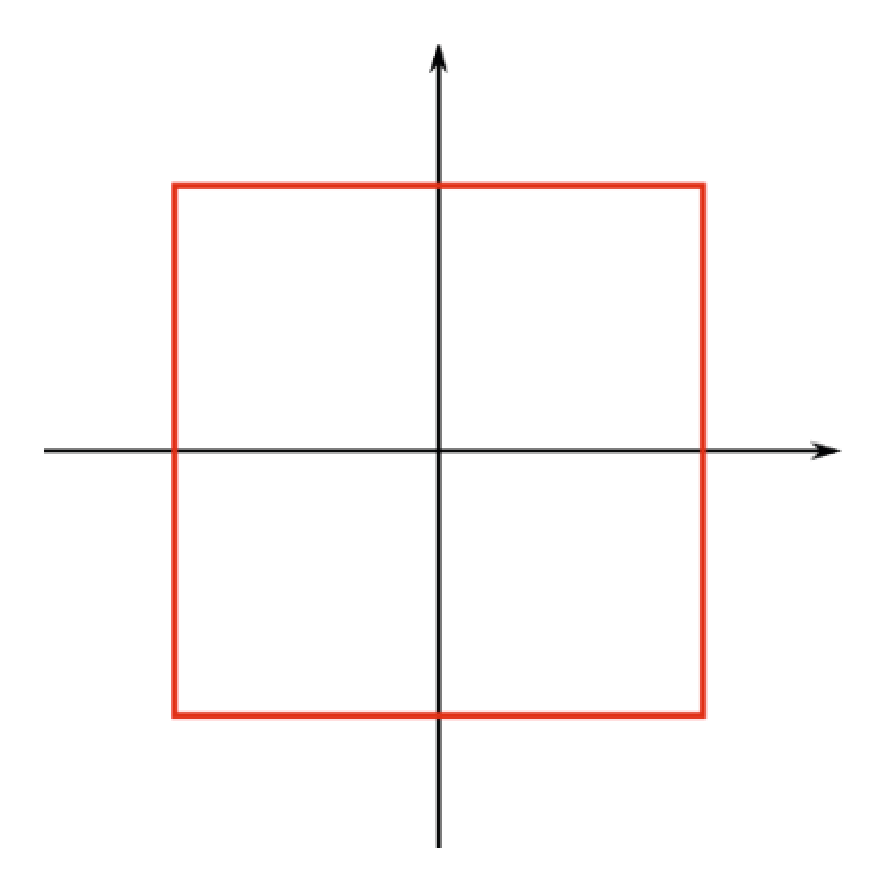
\includegraphics[scale=0.35]{fig3_1} 
		\figcaption{正方形}
	}
	
	\marginpar{
		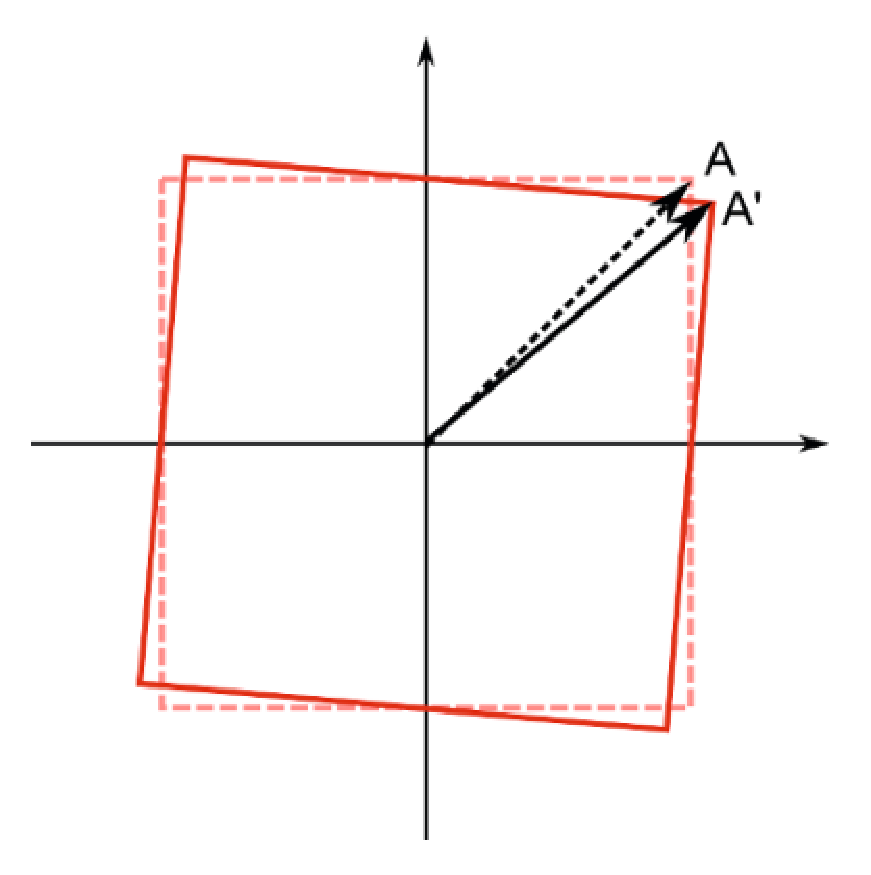
\includegraphics[scale=0.35]{fig3_2.eps}
		\figcaption{正方形绕中心顺时针旋转$5^\circ$}
	}
	
	注意不是所有旋转变换都对称。 我们关注顶点的变化就能看出来, 比如绕中心顺时针旋转$5^\circ$, 这个变换将顶点映射到原来正方形点集之外, 顶点$A$映射到了原来正方形集合之外的点$A'$。 因此这个旋转变换对正方形不具有对称性。 当然, 变换后的点集仍然是个正方形, 但却是不同的正方形(即不同点的集合)。 绕中心转$90^\circ$是对称的, 如图\ref{fig3.3}, 顶点$A$变换到点$B$, 等等, 原来的正方形点集变换到相同的集合。
	
	{
	\centering{
	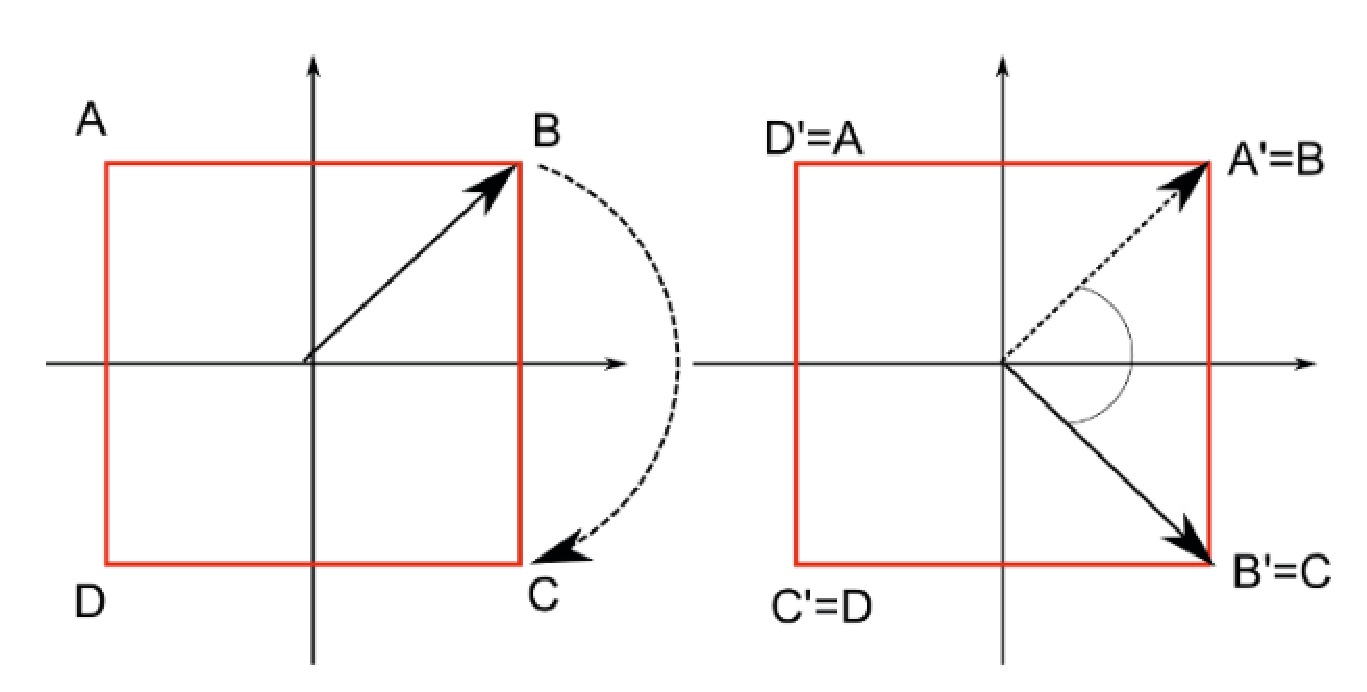
\includegraphics[scale=0.4]{fig3_3}
	\figcaption{正方形绕中心旋转$90^\circ$}
	\label{fig3.3}
	}}
	
	假如你看了一眼原来的正方形, 然后闭上眼睛, 这时有人把正方形做了一个变换。 如果你不能分辨这个正方形是否发生变化, 那么这个变换就是个对称变换。
	
	我们把所有使正方形不变的变换构成的集合称为群。 变换参数(本例中就是旋转角度)不能任意取值(而是取分立的数), 这个群称为离散群。
	
	\item 另一个例子是使单位圆不变的变换构成的集合。 类似地, 单位圆还是一些点构成的集合, 对称变换把这个集合映射到它自身。
	
	单位圆绕圆心旋转任意角度都不变。 换言之, 变换参数(这里就是旋转角度)可以取任意值, 因此这个群称为连续群。
\end{enumerate}
	\marginpar{
		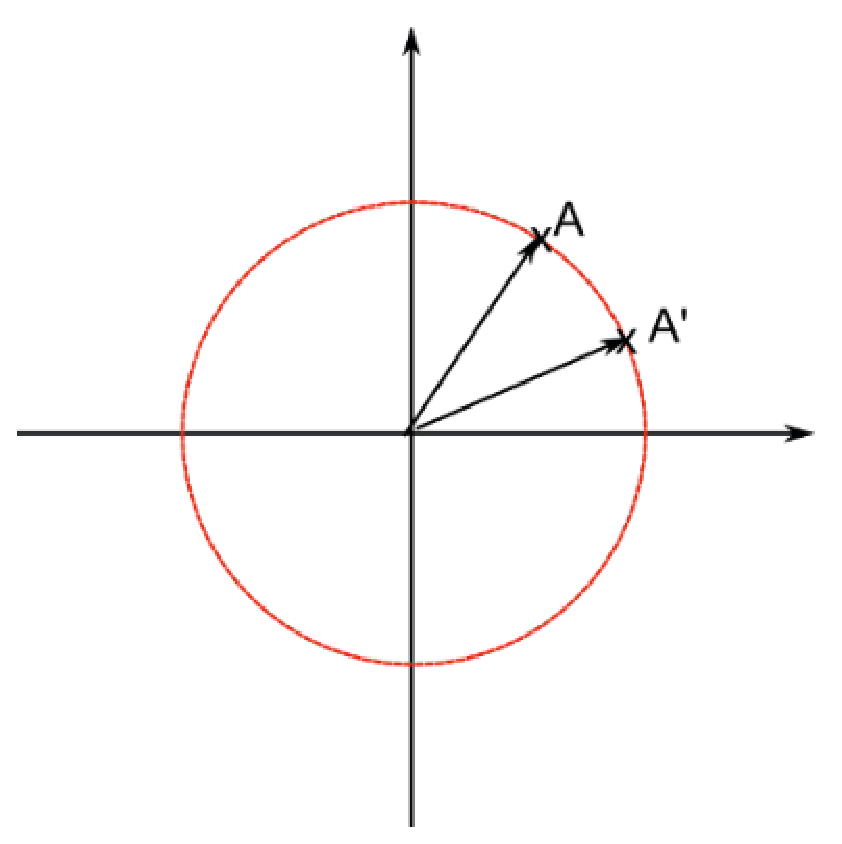
\includegraphics[scale=0.35]{fig3_4.eps}
		\figcaption{单位圆绕圆心旋转任意角度都不变}
	}

数学中除了几何图形之外还有好多别的都有对称性。 例如,对于向量, 我们可以考虑所有让向量长度不变的变换构成的集合。 看出本节开头对称性定义的普遍性了没? 对称性就是变换下的不变性。 非常幸运, 搞数学的早已建立了群论, 它可以研究所有类型的对称性\mpar{历史上数学家们建立群论最初是为了描述方程的对称性}。

为了让精确描述对称性的工具 --- 群的定义来的自然一点, 我们把对称性的定义用数学语言精炼一下:
\begin{itemize}
	\item 对某物什么也不做(比如转个$0^\circ$)当然也是对称变换(按照我们的对称性定义), 因此任何群都需要包含一个恒等变换(恒等元)。 在上面的例子里, 恒等元就是旋转$0^\circ$。
	
	\item 对某物先做变换再做逆变换的结果必须等于啥也不做。 因此对于群中的任意元素(简称群元), 必须有相应的逆元素。 按定义, 先做变换再做逆变换等于恒等变换。 例如先转$90^\circ$再转$-90^\circ$(先逆针再顺针转)与旋转$0^\circ$相同。
	
	\item 先做一个对称变换再做一个对称变换, 总体效果必须还是对称变换。 例如先旋转$90^\circ$再转$180^\circ$等于直接转$270^\circ$, 后者也是对称变换。 对称变换的这个性质称为封闭性。
	
	\item 对称变换之间必须满足结合律。 例如先转$90^\circ$再转$40^\circ$再转$110^\circ$与先转$130^\circ$再转$110^\circ$相同, 先转$90^\circ$再转$150^\circ$也一样。 用符号表示更加清楚:
	\begin{equation}\label{equ3.1}
	R(110^\circ) R(40^\circ) R(90^\circ) = R(110^\circ)\bigg( R(40^\circ)R(90^\circ) \bigg) = R(110^\circ) R(130^\circ)
	\end{equation}
	\begin{equation}\label{equ3.2}
	R(110^\circ) R(40^\circ) R(90^\circ) = \bigg( R(110^\circ) R(40^\circ) \bigg) R(90^\circ) = R(150^\circ) R(90^\circ)
	\end{equation}
	这个性质称为{\bf 结合律}。
	
	\item 我们要有规定两个群元(对称变换)怎样合体的规则, 它是个{\bf 二元运算}(两个群元合体成一个), 我们称它为{\bf 群乘法}。 
	
	在上面的例子里, 旋转变换的标准表示方法是用旋转矩阵\mpar{旋转矩阵见附录A.2.}, 两个群元(两个旋转矩阵, 或两个旋转操作)合体的规则是线性代数里的矩阵乘法。 同样的变换经常有不同的表示方法\mpar{例如, 二维平面旋转还可以用单位复数描述, 相应的群乘法是复数乘法。 稍后就讨论这一点。}, 群论非常系统性地概括了所有形式。 群论的分支 --- {\bf 表示论}就是研究相同变换的不同描述方式的, 我们在\ref{sec3.5}节学习表示论。
\end{itemize}

\ 

我们把上述群与对称变换的特征用严谨的数学语言表达, 再将它们提升为公理, 满足这些公理的数学结构就是一个群。 数学系的群论书可能更喜欢在开头就从天上掉下来这些公理。 必须指出满足群公理的结构可能是超级抽象的, 但我们现在只关注上面例子里的旋转变换那样的群。 \sout{因为我们是物理系的, 而且这是本物理书}

\ 

(我们通过对称变换的性质导出的)群公理\mpar{别担心怎么才能根据这些公理凑出一个群来。 搞物理的往往是从某个变换出发, 考察它是否符合群公理, 如果是\sout{经常是}那么就可以应用群论来解决问题。}: 

一个群就是一个集合$G$加上一个定义在$G$上的二元运算(群乘法)$\circ$, 当然$(G, \circ)$还要满足以下公理: 
\begin{itemize}
	\item 封闭性: 对于任意$g_1, g_2 \in G, g_1 \circ g_2 \in G$
	
	\item 单位元: 存在单位元$e \in G$使得对于所有$g \in G, g\circ e = g = e \circ g$
	
	\item 逆元: 对于任意$g \in G$, 存在相应的逆元$g^{-1} \in G$使得$g \circ g^{-1} = e = g^{-1} \circ g$
	
	\item 结合律: 对于任意$g_1, g_2, g_3 \in G, g_1 \circ (g_2 \circ g_3) = (g_1 \circ g_2) \circ g_3$ 
\end{itemize}

总结: 某物体在一些变换下保持不变, 这些变换组成\footnote{我在想这里该用`构成'还是`组成', 后来我觉得无所谓, 因为这不是初中化学...(分子构成物质, 元素组成物质...) --- 译者(SI)}的集合叫做对称群。 对于Minkowski时空, Minkowski度规\mpar{复习一下, Minkowski度规就是在Minkowski空间中用来计算距离和长度的工具, 见第二章。}在变换下保持不变, 相应的对称群称为Poincare群。

要注意群的定义完全与变换的物体是啥没有关系。 我们可以脱离特定物体而只研究对称变换本身, 群的定义将变换从物体中`提取'出来了。 这是非常有用的, 许多不同事物具有同样或同类的对称性。 群论让我们不用管变换的物体(圆还是正方形), 只研究变换(例如旋转)的普遍性质。


\section[二维旋转]{Rotations in two Dimensions\quad 二维旋转}
\label{sec3.2}
我们从一个简单而重要的例子开始学习群论。考虑那些让二维平面中的向量长度不变的对称变换。符合条件的有旋转和反射\mpar{当然还有平移。平移的数学描述与前两者有些不同,我们之后再讨论它。}。它们也是圆的对称变换,一个单位元旋转或反射之后还是单位圆。可见同一个群(对应一种变换)可以作用于不同类物体:圆(几何图形),或者向量。本节考虑向量,可以用旋转矩阵表示向量的旋转或反射,\mpar{旋转矩阵的推导见附录A.2.},将起点位于原点的向量绕原点逆时针旋转$\theta$角度的旋转矩阵为:
\begin{equation}
\label{equ3.3}
R_\theta = 
	\begin{pmatrix}
		\cos \theta & \sin \theta \\
		-\sin \theta & \cos \theta
	\end{pmatrix}
\end{equation}

关于$x$轴与$y$轴的反射变换用矩阵表示为:
\begin{equation}
\label{equ3.4}
P_x = 	\begin{pmatrix}
			-1 & 0 \\ 0 & 1
		\end{pmatrix}
\quad
P_y = 	\begin{pmatrix}
			1 & 0 \\ 0 & -1
		\end{pmatrix}
\end{equation}
将矩阵乘法作为群乘法$\circ$, 可以验证$R(\theta), P_x, P_y$与矩阵乘法符合群公理,因而构成一个群,亦即旋转与反射变换构成一个群。

可以用更抽象的方式表达‘所有让二维向量长度不变的变换’,向量长度就是向量与自身点乘的平方根($|a| = \sqrt{a \cdot a}$). 向量长度在变换$a \rightarrow a'$下不变意味着\footnote{等号上面的!只是起强调、提示作用 --- 译者(SI)}:
\begin{equation}
\label{equ3.5}
a' \cdot a' \stackrel{!}{=} a \cdot a
\end{equation}

将变换矩阵记作$\mathcal{O}$,变换即为$a \rightarrow a' = \mathcal{O}a$.
\begin{equation}
\label{equ3.6}
a \cdot a = a^{\mathrm{T}} a \rightarrow a'^{\mathrm{T}} a' = (\mathcal{O} a)^{\mathrm{T}} \mathcal{O} a = a^{\mathrm{T}} \mathcal{O}^{\mathrm{T}} \mathcal{O} a \stackrel{!}{=} a^{\mathrm{T}} a = a \cdot a
\end{equation}
由此可见,使向量长度不变的变换必须满足:
\begin{equation}
\label{equ3.7}
\mathcal{O}^{\mathrm{T}} \mathcal{O} = I
\end{equation}
其中$I$表示单位矩阵\mpar{ I = 
	\[\begin{pmatrix}
		1 & 0 \\ 0 & 1
	\end{pmatrix}\]}。前文的旋转和反射矩阵都满足此条件\mpar{例如\ref{equ3.3}式的矩阵,
	$R_\theta^{\mathrm{T}} R = 
	\begin{pmatrix}
		\cos \theta & -\sin \theta \\
		\sin \theta & \cos \theta
	\end{pmatrix}
	\begin{pmatrix}
		\cos \theta & \sin \theta \\
		-\sin \theta & \cos \theta
	\end{pmatrix}
	 = 
	 \begin{pmatrix}
		 \cos^2 \theta + \sin^2 \theta & 0 \\
		 0 & \sin^2 \theta + \cos^2 \theta
	 \end{pmatrix}
	 =
	 \begin{pmatrix}
		 1 & 0 \\ 0 & 1
	 \end{pmatrix}
	$
}%mpar
$2 \times 2$矩阵中所有满足\ref{equ3.7}式的矩阵构成了$\mathcal{O}(2)$群,即所有$2 \times 2$正交矩阵构成的群\mpar{严谨地说,任意$2 \times 2$正交矩阵可以表示为\ref{equ3.3}、\ref{equ3.4}式,或者它们的乘积的形式。}。我们可以找出这个群中描述旋转变换的那一部分(构成一个子群)。根据\ref{equ3.7}式:
\begin{align}
\det(\mathcal{O}^{\mathrm{T}} O ) = \det(O^{\mathrm{T}}) \det(O) \stackrel{!}{=} \det(I) = 1 \nonumber\\
\label{equ3.8}
(\det(\mathcal{O}))^2 \stackrel{!}{=} 1 \rightarrow \det{(\mathcal{O})} \stackrel{!}{=} \pm 1
\end{align}

$\det \mathcal{O} = 1$的矩阵对应旋转变换\mpar{见\ref{equ3.3}与\ref{equ3.4}式。反射矩阵的行列式等于$-1$。}

条件
\begin{align}
\label{equ3.9}
\mathcal{O}^{\mathrm{T}} \mathcal{O} = I \\
\label{equ3.10}
\det \mathcal{O} = 1
\end{align}
定义了$\mathcal{SO}(2)$群,`$\mathcal{S}$'表示‘特殊’(special),`$\mathcal{O}$'表示‘正交’(orthogonal)。

$\mathcal{SO}(2)$包含的旋转变换保持了坐标系的取向,即一个右手坐标系\mpar{右手坐标系与左手坐标系见附录A.5.}经旋转变换后还是右手系,而反射变换会改变它的取向。用线性代数的概念来说,我们规定$\mathcal{SO}(2)$中的矩阵行列式必须为$+1$。

\subsection[单位复数表示旋转变换]{Rotations with Unit Complex Numbers\quad 单位复数表示旋转变换}
\label{sec3.2.1}
还可以用单位复数来表示旋转变换:向量绕原点旋转$\theta$角可以表示为用单位复数$z$乘此向量(单位复数意为$z = a + ib$,$|z|^2 = z^* z = 1$)\mpar{上标$ ^*$表示复数的共轭复数:$z = a + ib \rightarrow z^* = a - ib$}。

所有单位复数构成一个群,称为$\mathcal{U}(1)$,群乘法即为复数乘法,不难验证它符合群公理。为了看出它与之前引入的$\mathcal{O}(3), \mathcal{SO}(3)$群的关系,我们将$\mathcal{U}(1)$群的条件 --- 单位复数表示为\mpar{定义中包含复数乘法的群的普遍性质见\ref{sec3.10}节的附录。}, $\forall \mathcal{U} \in \mathcal{U}(1)$:
\begin{equation}
\label{equ3.11}
\mathcal{U}^* \mathcal{U} = 1
\end{equation}
单位复数另一种形式是利用欧拉公式\mpar{附录B.4.2推导了传说中的欧拉公式。对任意复数$z = a + ib$, $a$称为$z$的实部,记为$\Re(z) = a$; $b$称为虚部,记为$\Im(z) = b$. 欧拉公式中$R_\theta$的实部为$\cos  \theta$, 虚部为$\sin \theta$.}:% Euler翻译为欧拉
\begin{equation}
\label{equ3.12}
R_\theta = \mathrm{e}^{i\,\theta} = \cos \theta + i\sin \theta
\end{equation}
$R(\theta)$的模(长度)为:
\begin{equation}
\label{equ3.13}
R_\theta^* R_\theta = \mathrm{e}^{-i\,\theta} \mathrm{e}^{i\,\theta} = \big( \cos \theta - i \sin \theta  \big) \big( \cos \theta + i \sin \theta \big) = 1
\end{equation}

\marginpar{
	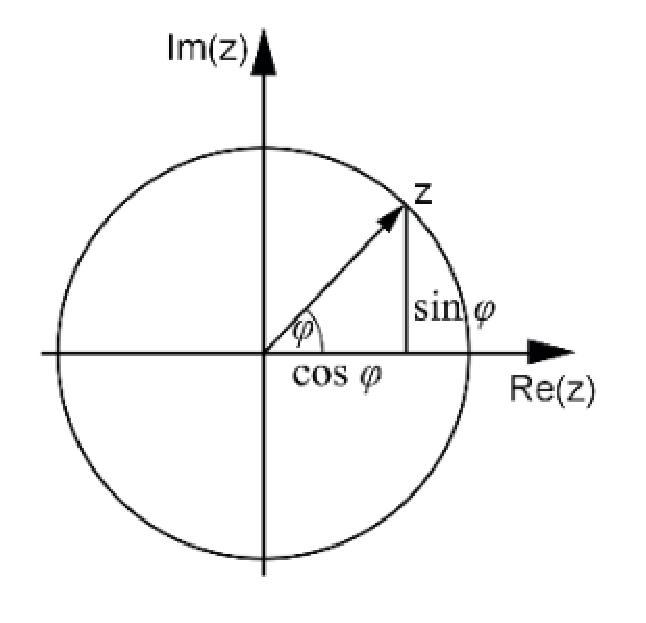
\includegraphics[scale=0.45]{fig3_5.eps} 
	\figcaption{单位复数在复平面的单位圆上}
	}

例:将向量$(3,  5)$旋转$90^\circ$:
\begin{equation}
\label{equ3.14}
z \rightarrow z' = \mathrm{e}^{i\, 90^\circ}z = \bigg( \underbrace{\cos 90^\circ}_{=0} + i\underbrace{\sin 90^\circ}_{=1} \bigg) (3 + 5i) = i(3 + 5i) = 3i - 5
\end{equation}

图3.6绘制了旋转前后的向量(复数),图中可见复数乘以$\mathrm{e}^{i\, 90^\circ}$旋转了$90^\circ$.
\marginpar{
	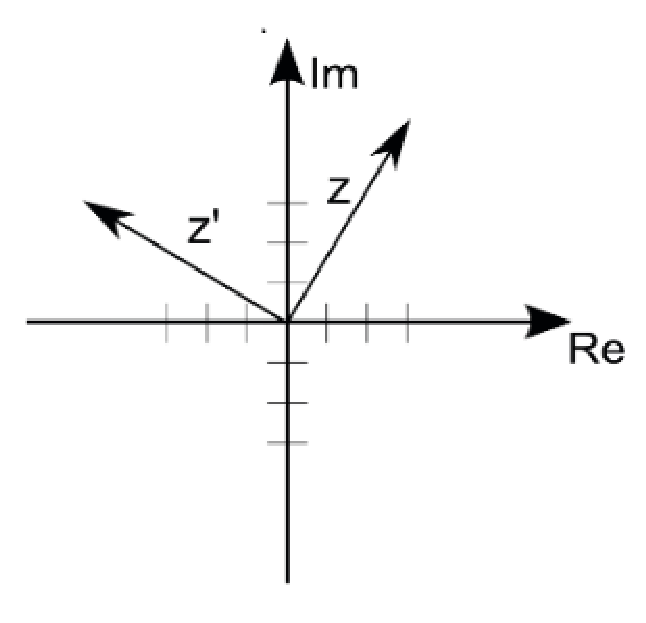
\includegraphics[scale=0.45]{fig3_6.eps} 
	\figcaption{复数通过乘以单位复数进行旋转}
	}
需要注意$\mathrm{e}^{i\, 90^\circ}$作用于(乘以)向量对应的复数而非向量本身。描述二维旋转只需要一个参数:旋转角$\phi$. 而复数有两个自由度(实部和虚部),因此我们加上单位复数的限制:$|z| = \text{实部}^2 + \text{虚部}^2 = 1$,只剩一个自由度。

描述二维旋转的两种方式 --- 单位复数与$2 \times 2$矩阵(矩阵元都是实数)通过如下方式关联。定义:
\begin{equation}
\label{equ3.15}
\mathbf{1} = 
	\begin{pmatrix}
		1 & 0 \\ 0 & 1
	\end{pmatrix}
,\quad
\mathbf{i} = 
	\begin{pmatrix}
		0 & -1 \\ 1 & 0
	\end{pmatrix}
\end{equation}
不难验证这样定义的$\mathbf{1, i}$仍然满足:
\begin{equation}
\mathbf{1}^2 = \mathbf{1},\quad \mathbf{i}^2 = -\mathbf{1},\quad \mathbf{1i} = \mathbf{i1} = \mathbf{i}
\end{equation}
这样单位复数对应的$2 \times 2$实数矩阵为\footnote{原文此式有误,译文已参照勘误表修改。}
\begin{equation}
\label{equ3.17}
R_\theta = \cos \theta + i\sin\theta = \cos \theta 
\begin{pmatrix}
	1 & 0 \\ 0 & 1
\end{pmatrix}
+ \sin \theta
\begin{pmatrix}
	0 & -1 \\ 1 & 0
\end{pmatrix}
=
\begin{pmatrix}
	\cos \theta & -\sin \theta \\
	\sin \theta & \cos \theta
\end{pmatrix}
\end{equation}
可见,定义了复单位$i \rightarrow \text{实矩阵}$的对应关系后,单位复数就回到了熟悉的旋转矩阵。还有一点要注意:旋转矩阵作用于向量(列矩阵),而我们将$i$与$2 \times 2$矩阵相联系,因此被旋转的向量(与一个复数对应)也将变成一个$2 \times 2$矩阵。

例:任意向量$(a, b)$对应的复数对应的$2 \times 2$矩阵为:
\begin{equation}
\label{equ3.18}
z = a + ib = a
\begin{pmatrix}
	1 & 0 \\ 0 & 1
\end{pmatrix}
+ b
\begin{pmatrix}
	0 & -1 \\ 1 & 0
\end{pmatrix}
=
\begin{pmatrix}
	a & -b \\ b & a
\end{pmatrix}
\end{equation}
将旋转矩阵作用于$z$:
\begin{eqnarray}
\label{sec3.19}
	z' &=& \begin{pmatrix}
			a' & -b' \\ b' & a'
		 \end{pmatrix}
	= R_\theta z = 
		\begin{pmatrix}
			\cos \theta & -\sin \theta \\
			\sin \theta & \cos \theta
		\end{pmatrix}
		\begin{pmatrix}
			a & -b \\ b & a
		\end{pmatrix}
	\nonumber \\
	&=& \begin{pmatrix}
			a\cos\theta - b\sin \theta & - b\cos \theta - a \sin \theta \\
			a\sin \theta + b\cos \theta & -b \sin \theta + a \cos \theta
		\end{pmatrix}
\end{eqnarray}
由上式可得
\begin{align}
\label{equ3.20}
a' &= a \cos \theta - b \sin \theta \\
\label{equ3.21}
b' &= a \sin \theta + b \cos \theta
\end{align}
这与旋转矩阵作用于向量(列矩阵形式)相同:
\begin{equation}
\label{equ3.22}
	\begin{pmatrix}
		\cos \theta & -\sin \theta \\
		\sin \theta & \cos \theta
	\end{pmatrix}
	\begin{pmatrix}
		a \\ b
	\end{pmatrix}
	=
	\begin{pmatrix}
		a \cos \theta - b \sin \theta \\
		a \sin \theta + b \cos \theta
	\end{pmatrix}
	=
	\begin{pmatrix}
		a' \\ b'
	\end{pmatrix}
\end{equation}
我们看到这两种表示方法是一回事儿,用数学术语来说,$\mathcal{SO}(2)$与$\mathcal{U}(1)$间有一个同构映射\mpar{如果映射$\Pi: G \rightarrow G'$是一一映射,并且满足:$\forall g_1, g_2 \in G, \Pi(g_1) \circ \Pi(g_2) = \Pi(g_1 \circ g_2)$, 则$\Pi$就是同构映射,并且称群$G, G'$是同构的。}。这一点太重要了,之后的篇幅会不断出现这种思想。

下面研究三维旋转,尝试找出它的两种描述方法。

\section[三维旋转]{Rotations in three Dimensions\quad 三维旋转}
\label{sec3.3}
三维空间向量旋转变换当然可以用$3 \times 3$旋转矩阵\footnote{原文公式有误,译文已按勘误表改正。}:
\begin{align}
R_x =
	\begin{pmatrix}
		1 & 0 & 0 \\
		0 & \cos \theta & -\sin \theta \\
		0 & \sin \theta & \cos \theta
	\end{pmatrix}
\quad
R_y = 
	\begin{pmatrix}
		\cos \theta & 0 & \sin \theta \\
		0 & 1 & 0 \\
		-\sin \theta & 0 & \cos \theta
	\end{pmatrix}
\nonumber \\
\label{equ3.23}
R_z =
	\begin{pmatrix}
		\cos \theta & -\sin \theta & 0 \\
		\sin \theta & \cos \theta & 0 \\
		0 & 0 & 1
	\end{pmatrix}
\end{align}
类比$\mathcal{SO}(2)$群,上面三个矩阵构成了$\mathcal{SO}(3)$群的一组基\mpar{基的概念见附录A.1.}。这意味着$\mathcal{SO}(3)$中的任意群元(矩阵)都可以写为$R_x, R_y, R_z$的线性组合,且系数唯一。
将向量
\begin{equation*}
\vec{v} = \begin{pmatrix}
			1 \\ 0 \\ 0
		\end{pmatrix}
\end{equation*}
绕$z$轴旋转\mpar{三维向量旋转的一般情况的推导见附录A.2.}就是用旋转矩阵乘以向量:
\begin{equation}
\label{equ3.24}
R_z(\theta) \vec{v} = 
	\begin{pmatrix}
		\cos \theta & -\sin \theta & 0 \\
		\sin \theta & \cos \theta & 0 \\
		0 & 0 & 1
	\end{pmatrix}
	\begin{pmatrix}
		1 \\ 0 \\ 0
	\end{pmatrix}
=
	\begin{pmatrix}
		\cos \theta \\ \sin \theta \\ 0
	\end{pmatrix}
\end{equation}
为找出描述三维旋转的第二法,我们尝试把复数的概念扩展到三维空间。首先试着把$2$维的复数(实部虚部两个自由度)扩展为$3$维复数,但前人探索发现没有$3$维的,但存在$4$维‘复数’,称为{\bf 四元数(quaternions)}。下面就会看到四元数正是描述三维旋转的第二法,并且它还能深刻揭示宇宙 --- 四维时空的规律。描述三维旋转需要三个参数(绕$x,y,z$轴的旋转角),而四元数有四个参数,这与二维旋转的情况类似\mpar{单位复数描述二维旋转。}。四元数加上单位长度的限制 ---单位四元数(三个自由参数)能够描述三维旋转。

\subsection[四元数]{Quaternions\quad 四元数}
\label{sec3.3.1}
我们类比复数来构造四元数,复数只有一个虚单位$i$,而四元数里定义三个虚单位,记作$\mathbf{i,j,k}$,它们仍然满足
\begin{equation}
\label{equ3.25}
\mathbf{i}^2 = \mathbf{j}^2 = \mathbf{k}^2 = -1
\end{equation}
这样任意一个四元数$q$表示为
\begin{equation}
\label{equ3.26}
q = a\mathbf{1} + b\mathbf{i} + c\mathbf{j} + d\mathbf{k}
\end{equation}
其中$a, b, c, d \in \mathbb{R}$, $\mathbf{1}$就是正常的实数1。\footnote{$\mathbf{1,i,j,k}$用黑体表示是为了强调它们是四元数的基。---译者(SI)}

要想定义四元数间的乘法,必须定义虚单位间的乘法规则,比如$\mathbf{ij} = ?$. 为此再定义
\begin{equation}
\label{equ3.27}
\mathbf{ijk} = -1
\end{equation}
这样虚单位间的乘法就没问题了,例如,为导出$\mathbf{ij} = \mathbf{k}$, 在\ref{equ3.27}式等号两侧右乘$\mathbf{k}$:
\begin{equation}
\label{equ3.28}
\mathbf{ij} \underbrace{\mathbf{kk}}_{= -1} = -\mathbf{k} \rightarrow \mathbf{ij} = \mathbf{k}
\end{equation}

单位四元数$q = a\mathbf{1} + b\mathbf{i} + c\mathbf{j} + d\mathbf{k}$满足\mpar{符号$\dag$称为`dagger',表示转置加取复共轭,即$a^\dag = (a^*)^T$。实数向量间的点乘定义为$a \cdot b = a^T b$, 向量用列矩阵表示,其转置为行矩阵,于是点乘的定义符合矩阵乘法规则。四元数对应的列矩阵含复数,为使四元数与它自身相乘结果为实数(实数结果可表示‘长度’),在转置之外还加上取复共轭。}:
\begin{align}
q^\dag q &\stackrel{!}{=} 1 \nonumber\\
\label{equ3.29}
\rightarrow (a\mathbf{1} - b\mathbf{i} - c\mathbf{j} - d\mathbf{k}) (a\mathbf{1} +& b\mathbf{i} + c\mathbf{j} + d\mathbf{k}) = a^2 + b^2 + c^2 + d^2 \stackrel{!}{=} 1
\end{align}

就像单位复数构成一个群(群乘法为复数乘法)那样,单位四元数也构成一个群(群乘法为四元数乘法)。

类似于我们将二维复数与$2 \times 2$实数矩阵建立联系的做法,四元数也可如此 --- 将四个基$\mathbf{1,i,j,k}$与合适的矩阵一一对应。其中一种方法(还有别的方式)是将它们与$2 \times 2$复数矩阵对应:
\begin{align}
\mathbf{1} = \begin{pmatrix}
				1 & 0 \\ 0 & 1
			 \end{pmatrix}
\quad &, \quad
\mathbf{i} = \begin{pmatrix}
				0 & 1 \\ -1 & 0 
			 \end{pmatrix}
\nonumber \\
\label{equ3.30}
\mathbf{j} = \begin{pmatrix}
				0 & -i \\ -i & 0
			 \end{pmatrix}
\quad &, \quad
\mathbf{k} = \begin{pmatrix}
				i & 0 \\
				0 & -i
			 \end{pmatrix}
\end{align}
不难验证上式满足四元数乘法,比如\ref{equ3.25}、\ref{equ3.27}式。这样任意一个四元数都可用矩阵表示为:
\begin{equation}
\label{equ3.31}
q = a\mathbf{1} + b\mathbf{i} + c\mathbf{j} + d\mathbf{k} = \begin{pmatrix}
	a + di & -b - ci \\
	b - ci & a - di
	\end{pmatrix}
\end{equation}
由上式可见
\begin{equation}
\label{equ3.32}
\det(q) = a^2 + b^2 + c^2 + d^2
\end{equation}
上式与\ref{equ3.29}式比较可以发现单位四元数对应的矩阵的行列式为$1$。因此单位四元数对应的$2 \times 2$复数矩阵$\mathcal{U}$满足:
\begin{equation}
\label{equ3.33}
\mathcal{U}^\dag \mathcal{U} = 1, \quad \text{且} \det(\mathcal{U}) = 1
\end{equation}
注意\ref{equ3.30}式中的矩阵是线性独立的\mpar{线性独立的概念见附录A.1.},它们构成群$\mathcal{SU}(2)$的基。与之前相同,$\mathcal{S}$表示特殊(special),含义为$\det (\mathcal{U}) = 1$;$\mathcal{U}$表示幺正(unitary)\mpar{进一步介绍见本章附录 --- \ref{sec3.10}节。},即$\mathcal{U}^\dag \mathcal{U} = 1$。任意单位四元数都唯一对应$\mathcal{SU}(2)$群中的一个群元。

$\mathcal{SU}(2)$群如何与三维旋转联系?事情正在起变化,$\mathcal{SU}(2)$群与$\mathcal{SO}(3)$\mpar{$\mathcal{SO}(3)$群就是三维旋转矩阵构成的群。}之间的对应关系并不像二维旋转中$\mathcal{U}(1)$与$\mathcal{SO}(2)$那样简单。

2维虚数$z = a + ib$与2维向量很容易对应。单位复数保证了矢量长度在旋转变换下不变\mpar{注意这里的$R$表示一个单位复数,即$R^* R = 1$, $R$与复数$z$相乘就将$z$进行旋转变换。}:$(Rz)^* Rz = z^* R^* Rz = z^* z$。四元数有$4$个参数,它与三维向量的对应关系是并不明显。我们尝试将三维向量$\vec{v} = (x, y, z)$定义为如下四元数\footnote{注意下式中的$\mathbf{ijk}$是四元数的‘基’而非三维直角坐标系的基矢。 --- 译者}:
\begin{equation}
\label{equ3.34}
v \equiv x\mathbf{i} + y\mathbf{j} + z\mathbf{k}
\end{equation}
利用前述四元数的矩阵表示可得:
\begin{equation}
\label{equ3.35}
\det(v) = x^2 + y^2 + z^2
\end{equation}
于是保持向量$(x, y, z)$长度不变的变换就对应于保持矩阵行列式不变的矩阵变换。而{\bf 单位}四元数对应矩阵都具有{\bf 单位}行列式,它与任意矩阵相乘不改变该矩阵的行列式\footnote{利用$\det(AB) = \det(A)\det(B)$, --- 译者}。进展很顺利,但现在有个微妙的状况:继续猜想下去,我们会认为用单位四元数$u$旋转向量(对应的四元数)$v$直接用$u$乘以$v$就可以了(按照四元数乘法规则)。但细想起来这却不行,因为根据\ref{equ3.34}式,我们把任意三维向量对应的四元数定义在$\mathbb{R}\mathbf{i} + \mathbb{R}\mathbf{j} + \mathbb{R}\mathbf{k}$的范围内,$u$与$v$的四元数乘积会超出这个范围,这样向量旋转后可能不是个向量!这当然不行。

事实上,旋转变换表示为:
\begin{equation}
\label{equ3.36}
v' = q^{-1} v q
\end{equation}
其中$v$, $v'$分别为旋转前后的向量,$q$为表示旋转的单位四元数。

这样我们终于实现了描述三维旋转的第二法 --- 单位四元数。

例:定义$u$是$\mathbb{R}\mathbf{i} + \mathbb{R}\mathbf{j} + \mathbb{R}\mathbf{k}$中的某一单位向量,则任意单位四元数$t$可表示为:
\begin{equation}
\label{equ3.37}
t = \cos \theta +  u\sin \theta
\end{equation}
利用\ref{equ3.34}式,任意三维向量$\vec{v}$可表示为:
\begin{equation}
\label{equ3.38}
\vec{v} = (v_x, v_y, v_z)^T = v_x \mathbf{i} + v_y \mathbf{j} + v_z \mathbf{k} \underbrace{=}_{\ref{equ3.31}\text{式}} \begin{pmatrix}
		iv_z & -v_x - iv_y \\
		v_x - iv_y & -iv_z
	\end{pmatrix}
\end{equation}

简明起见我们举个特例,把向量$\vec{v} = (1, 0, 0)^T$绕$z$轴旋转。
\begin{align}
\label{equ3.39}
\vec{v} &= (1, 0, 0)^T \rightarrow v = 1\mathbf{i} + 0\mathbf{j} + 0\mathbf{k} = 
	\begin{pmatrix}
		0 & -1 \\ 1 & 0
	\end{pmatrix}
\\
\label{equ3.40}
R_z(\theta) &= \cos \theta \mathbf{1} + \sin \theta \mathbf{k} =
	\begin{pmatrix}
		\cos \theta + i\sin \theta & 0 \\
		0 & \cos \theta - i\sin \theta
	\end{pmatrix}
\end{align}
上式也可用欧拉公式写出\mpar{欧拉公式的推导见附录B.4.2}:
\begin{equation}
\label{equ3.41}
\mathrm{e}^{ix} = \cos x + i\sin x
\Rightarrow
R_z(\theta) = \begin{pmatrix}
				\mathrm{e}^{i\theta} & 0 \\
				0 & \mathrm{e}^{-i\theta}
			  \end{pmatrix}
\end{equation}
四元数旋转矩阵的逆矩阵为:
\begin{equation}
\label{equ3.42}
R_z^{-1} (\theta) = 
	\begin{pmatrix}
		\cos \theta - i\sin \theta & 0 \\
		0 & \cos \theta + i\sin \theta
	\end{pmatrix}
=
	\begin{pmatrix}
		\mathrm{e}^{-i\theta} & 0 \\
		0 & \mathrm{e}^{i\theta}
	\end{pmatrix}
\end{equation}
根据\ref{equ3.36}式旋转向量$v$;
\begin{align}
v' &= R_z^{-1} (\theta) v R_z(\theta) =
	\begin{pmatrix}
		\mathrm{e}^{-i\theta} & 0 \\
		0 & \mathrm{e}^{i\theta}
	\end{pmatrix}
	\begin{pmatrix}
	0 & -1 \\ 1 & 0
	\end{pmatrix}
	\begin{pmatrix}
		\mathrm{e}^{i\theta} & 0 \\
		0 & \mathrm{e}^{-i\theta}
	\end{pmatrix}
\nonumber \\
\label{equ3.43}
&= \begin{pmatrix}
		0 & -\mathrm{e}^{-i 2\theta} \\
		\mathrm{e}^{i 2\theta} & 0
	\end{pmatrix}
= \begin{pmatrix}
		0 & -\cos (2\theta) + i\sin (2\theta) \\
		\cos (2\theta) + i\sin (2\theta) & 0
  \end{pmatrix}
\end{align}
另一方面,向量$v'$用四元数表示为:
\begin{equation}
\label{equ3.44}
v' = 
	\begin{pmatrix}
		iv'_z & -v'_x - iv'_y \\
		v'_x - iv'_y & -iv'_z
	\end{pmatrix}
\end{equation}
上式与\ref{equ3.43}式比较可得:
\begin{equation}
\label{equ3.45}
v'_x = \cos(2\theta),\quad v'_y = -\sin (2\theta),\quad v'_z = 0
\end{equation}
所以
\begin{equation}
\label{equ3.46}
\rightarrow \vec{v'} = \big( \cos(2\theta), -\sin (2\theta), 0 \big)^T
\end{equation}
由上式可见从$\vec{v}$到$\vec{v}'$确实进行了旋转\mpar{见\ref{equ3.24}式,那里我们用三维旋转矩阵旋转向量。},但是要注意,上式表示我们没有把$\vec{v}$旋转$\theta$角度,而是旋转了$2\theta$!因此我们定义$\phi \equiv 2 \theta$, 这样$\phi$表示真正的旋转角,$\ref{equ3.37}$重写为:
\begin{equation}
\label{equ3.47}
t = \cos \left( \frac{\phi}{2} \right) + \sin \left(\frac{\phi}{2} \right) u
\end{equation}

这样定义的单位四元数与三维旋转矩阵之间的关系并非一一对应的,而是两个单位四元数描述同一个旋转,例如\mpar{将向量旋转$\pi$与旋转$3\pi = \pi + 2\pi$相同。换言之:两个单位四元数$u$与$-u$对应同一变换:旋转$\pi$.}:

{
\centering
\setlength{\unitlength}{0.8cm}
\begin{picture}(6, 4.5)\thicklines
\put(0.5, 3){\makebox(2.5, 1.2){\text{$t_{\phi = \pi} = u$}}}
\put(5.5, 3){\makebox(2.5, 1.2){\text{$t_{\phi = 3\pi} = -u$}}}

\put(1.7, 3.2){\vector(1, -1){1.4}}
\put(6.0, 3.2){\vector(-1, -1){1.4}}
\put(2.8, 0.8){\makebox(2.5, 1.2){\text{将向量旋转$\pi$}}}
\end{picture}
}

因此$\mathcal{SU}(2)$群称为$\mathcal{SO}(3)$群的{\bf 双覆盖}。一个$\mathcal{SU}(2)$中的群元对应$\mathcal{SO}(3)$的哪个群元是很明确的,反过来就不行,因为$\mathcal{SO}(3)$中的一个群元对应$\mathcal{SU}(2)$中的两个。这并非仅有数学意义,稍后就会看到,在物理上,一个能覆盖别的群的群往往更加深刻\mpar{剧透:Lorentz群的双覆盖蕴含{\bf 自旋}概念,而Lorentz群自身并不具有。自旋是指粒子的某种内禀角动量,它是粒子最重要的特征之一。自旋在小节\ref{sec4.5.4}和\ref{sec8.5.5}详述。}。

给定某个群,为了找出能覆盖这个群的群,我们需要学习Lie代数 --- Lie理论的利器,下一节就讲Lie代数。

注意我们把三维向量对应到四元数集$\mathbb{R}\mathbf{i} + \mathbb{R}\mathbf{j} + \mathbb{R}\mathbf{k}$中,因此四元数的一个参数没有用到,这是相对论的伏笔。比如将时间$t$考虑进来后,四维‘向量’与四元数对应的十分自然,就像二维复数与二维向量之间那样:$v = t\mathbf{1} + x\mathbf{i} + y\mathbf{j} + z\mathbf{k}$。纯数学的观点鼓励我们使用4维向量。如果我们想描述四维旋转(因为我们目前认为宇宙是$3+1$四维时空),应该怎么办?有两个选择:
\begin{itemize}
	\item 再去找更高维的‘复数’,或者:
	\item 再用四元数试试看。
\end{itemize}
从刚才的遐想可以看出四元数与四维旋转有着暧昧的联系。任意四维旋转需要$6$个参数表示\mpar{四维旋转矩阵$\mathcal{O}$($4 \times 4$)有$16$个参数,条件$\mathcal{O}^T \mathcal{O} = 1$与$\det(\mathcal{O}) = 1$将$16$个参数限制为$6$个自由参数。},没有$7$维复数,这样‘单位7维复数描述6个参数的四维旋转’就行不通了。我们注意到{\bf 两个}单位四元数正好有$6$个自由参数。因此两个单位四元数很可能可以描述四维旋转。之后会看到,两个$\mathcal{SU}(2)$群与四维旋转群确实存在千丝万缕的联系。

\section[Lie代数]{Lie Algebras\quad Lie代数}
\label{sec3.4}
Lie理论是研究连续对称的理论。连续对称的例子可见本章开头讨论的单位圆的旋转对称性。连续性意味着存在无限接近于恒等变换(恒等变换:什么都不干)的群元。相对的,离散群的群元个数是可数的,不存在无限接近于恒等元的群元。例如把正方形绕中心转$0.000001^\circ$,这与恒等变换(转$0^\circ$)非常接近,但它不是正方形的恒等变换。而把圆绕圆心转$0.000001^\circ$就是对称的。圆的对称群(对称变换组成的群)是连续的,因为变换参数(旋转角)可以取任意(连续)的值。用数学符号来表示:把恒等元记作$I$,无限接近恒等元的群元$g$可表示为:
\begin{equation}
\label{equ3.48}
g(\epsilon) = I + \epsilon X
\end{equation}
其中$\epsilon$表示小量(数学总是用$\epsilon$表示小量),$X$称为生成元,稍后就讨论它。这样一个轻微的小变换作用在物体上几乎啥也不变,有时称$g(\epsilon)$为无穷小变换。把无穷小变换重复许多次就能得到一个有限大小的变换。以旋转为例:许多朝同一方向小旋转等效于一次有限大的旋转。用数学语言来说,我们可以将无穷小变换重复许多次:
\begin{equation}
\label{equ3.49}
h(\theta) = \underbrace{(I + \epsilon X)(I + \epsilon X) \dots (I + \epsilon X)}_{k\text{个}(I + \epsilon X)} = (I + \epsilon X)^k
\end{equation}
其中$k$表示无穷小变换重复的次数。如果$\theta$表示有限大的旋转角,比如$50^\circ$什么的,然后$N$表示超大的数,则无限接近于恒等变换的旋转变换可表示为:
\begin{equation}
\label{equ3.50}
g(\frac{\theta}{N}) = I + \frac{\theta}{N} X
\end{equation}
要使上式表示的变换尽可能小,则让$N$尽可能大,令$N \rightarrow \infty$。为了从这样一个无穷小变换得到一个有限变换,需要把无穷小变换重复无限多次,即:
\begin{equation}
\label{equ3.51}
h(\theta) = \lim_{N \rightarrow \infty} \left( I + \frac{\theta}{N}X \right)^N
\end{equation}
微积分告诉我们这个极限就是指数函数\mpar{\ref{equ3.51}式经常用作指数函数的定义。指数的级数表示与\ref{equ3.51}式等价性的证明见附录B.4.1. 这在几乎所有的数学分析课本中都能找到。}:
\begin{equation}
\label{equ3.52}
h(\theta) = \lim_{N \rightarrow \infty} \left( I + \frac{\theta}{N}X \right)^N = \mathrm{e}^{\theta X}
\end{equation}
上式有$X$产生了有限变换$h(\theta)$的感觉,因此$X$成为{\bf 生成元}。生成元的定义之后详述,下面先从另一个角度看这个问题。

考虑某个用矩阵表示的连续变换群,对任意群元,在恒等元$I$处做Taylor展开\mpar{如果你从未听说过Taylor展开或Taylor级数,作者推荐你看一看附录B.3. \sout{而译者建议你学了微积分再来}}。
\begin{equation}
\label{equ3.53}
h(\theta) = I + \frac{dh}{d\theta} \Bigg|_{\theta = 0} \theta + \frac{1}{2} \frac{d^2 h}{d \theta^2} \Bigg|_{\theta = 0} \theta^2 + \dots = \sum_n \frac{1}{n!} \frac{d^n h}{d \theta^n} \Bigg|_{\theta = 0} \theta^n
\end{equation}

利用指数函数的级数展开可将上式的级数表示为更紧凑的形式\mpar{附录B.4.1中有推导}:
\begin{equation}
\label{equ3.54}
h(\theta) = \exp \left( \frac{dh}{d\theta}\Big|_{\theta = 0} \theta \right) \equiv \sum_n \frac{1}{n!} \frac{d^n h}{d \theta^n}\Bigg|_{\theta = 0} \theta^n
\end{equation}
这与之前的描述有联系。比较上式与\ref{equ3.52}式可得:
\begin{equation}
\label{equ3.55}
X = \frac{dh}{d\theta}\Bigg|_{\theta = 0}
\end{equation}

蕴含在上述推导中的思想是:通过研究群中重要的无穷小元素 --- {\bf 生成元}(上面的$X$)就能获得群的许多重要信息。

矩阵Lie群(记作$G$)的Lie代数就是下面的集合:
\[ 
\Big\{X \Big| \text{若}\mathrm{e}^X \in G \Big\}
\]
即如果$X$满足$\mathrm{e}^X$是$G$的群元,则$X$就是$G$的Lie代数(它是一个集合!)中的元素。这个简单定义只对矩阵Lie群管用。之后我们引入Lie代数的一般定义。

上面的矩阵Lie群的Lie代数的定义用数学语言表述为\mpar{群$G$的Lie代数通常用哥特体活字(Fraktur)字母$\mathfrak{g}$表示。}:

{ \it
$n \times n$矩阵Lie群$G$的Lie代数$\mathfrak{g}$是满足如下条件的$n \times n$矩阵$X$的集合:

	{\begin{center}
		$\mathrm{e}^{tX} \in G, t \in \mathbb{R}$
	\end{center}
	}
}

根据群的定义,群无非是一些变换的集合。群乘法$\circ$告诉我们群元之间怎样合体。矩阵Lie群的群乘法就是矩阵乘法,我们可能naive地认为Lie代数的元素之间采用相同的方式合体($\circ$),但这并不正确!诚然,(矩阵Lie群的)Lie代数的元素都是矩阵\mpar{Lie群理论的著名定理 --- Ado定理(Ado's Theorem)告诉我们任意Lie代数与矩阵Lie代数同构。},但两个Lie代数的矩阵乘法的结果往往不再是Lie代数的元素。Lie代数元素间有另外的合体规则,当然它与原来群的群乘法直接有关。

Lie群乘法与Lie代数合体法则之间的关系由著名的Baker-Campbell-Hausdorff公式(以下简称BCH公式)给出\mpar{我们不讲这个公式的证明,在大多数关于Lie理论的教材都能找到,比如 William Fulton and Joe Harris. Representation Theory: A First Course. Springer, 1st corrected edition, 8 1999. ISBN 9780387974958}:
\begin{equation}
\label{equ3.56}
\mathrm{e}^X \circ \mathrm{e}^Y = \mathrm{e}^{X + Y + \frac{1}{2}[X, Y] + \frac{1}{12} \big[X, [X, Y]\big] - \frac{1}{12} \big[Y, [X, Y]\big] + \dots  }
\end{equation}

其中\mpar{重复一下,群$G$的Lie代数通常用哥特体字母$\mathfrak{g}$表示。}$X, Y \in \mathfrak{g}$, 即$X, Y$是群$G$的生成元。$\mathrm{e}^X, \mathrm{e}^Y$是$G$的群元,把它们分别记作$g, h$,这样上式写成:
\begin{equation}
\label{sec3.57}
\underbrace{g}_{\in G} \circ \underbrace{h}_{\in G} = \mathrm{e}^X \circ \mathrm{e}^Y = \underbrace{\mathrm{e}^{ X + Y + \frac{1}{2} [X, Y] + \frac{1}{12}\big[X, [X, Y]\big] - \frac{1}{12} \big[Y, [X, Y]\big] + \dots }}_{\in G}
\end{equation}

上式等号右侧是群的一个群元,可见两个群元($g,h$)相乘可表示为一些Lie代数元素的和(再取指数)。上两式出现的新运算$[,]$称为{\bf Lie括号},对于矩阵Lie群,$[X, Y] = XY - YX$,$[X, Y]$称为$X, Y$的对易子。注意$XY$和$YX$一般不是Lie代数的元素,但它们的差一定是\mpar{John Stillwell. Naive Lie Theory. Springer, 1st edition, August 2008a. ISBN 978-0387782140 里面有漂亮的证明。}!

由BCH公式可知Lie代数元素间的乘法规则是Lie括号$[,]$,而非最初认为的矩阵乘法。就像群在群乘法$\circ$运算(矩阵群的$\circ$就是矩阵乘法)下封闭那样,我们称Lie代数在Lie括号运算下封闭。集合在某运算下封闭的含义是集合的任意两个元素进行该运算所得结果仍在此集合内\mpar{用数学语言表示封闭性:$\forall g, h \in G$, $g \circ h \in G$。 对于$X, Y \in \mathfrak{g}, [X, Y] \in \mathfrak{g}, X \circ Y \notin \mathfrak{g}$}。

在学习一个Lie代数的例子之后,我们将讨论Lie代数的现代定义。现代定义是从群的生成元在Lie括号运算下的行为来定义的。利用更广泛的现代定义就能看出哪些不同的群具有{\bf 相同的}Lie代数,只从上面的Lie代数定义出发看不出这一点来。因此Lie代数的新定义能让我们更深刻地认识一种变换的基本特征。同一Lie代数可对应许多Lie群,Lie理论的一条重要定理告诉我们这其中有一个{\bf 特别的}Lie群。引入Lie群的现代定义之后上面所说的就具体起来了。

下面我们就举一个从给定的群导出相应Lie代数的例子。

\subsection[$\mathcal{SO}(3)$群的生成元与Lie代数]{The Generators and Lie Algebra of $\mathcal{SO}(3)$\quad $\mathcal{SO}(3)$群的生成元与Lie代数}
\label{sec3.4.1}
$\mathcal{SO}(3)$群的定义为(\ref{equ3.10}式):
\begin{equation}
\label{equ3.58}
\mathcal{O}^T \mathcal{O} \stackrel{!}{=} I , \quad \det(\mathcal{O}) \stackrel{!}{=} 1
\end{equation}

任意群元$\mathcal{O}$用相应的生成元$J$表示为:
\begin{equation}
\label{equ3.59}
\mathcal{O} = \mathrm{e}^{\phi J} % 这里似乎应该用\phi(原文为\Phi),因为(3.69)式是用\phi表示的
\end{equation}

上式带入群的第一个定义条件得:
\begin{equation}
\label{equ3.60}
\mathcal{O}^T \mathcal{O} = \mathrm{e}^{\phi J^T} \mathrm{e}^{\phi J} \stackrel{!}{=} 1 \quad \rightarrow \quad J^T + J \stackrel{!}{=} 0
\end{equation}
带入第二个定义条件,再利用等式\mpar{$\tr(A)$表示矩阵$A$的迹,也就是$A$的主对角线上所有元素的和。例如\[A = \begin{pmatrix} A_{11} & A_{12} \\ A_{21} & A_{22} \end{pmatrix}\]的迹为$\tr(A) = A_{11} + A_{22}$。}$\det(\mathrm{e}^A) = \mathrm{e}^{\tr(A)}$得:
\begin{align}
\det(\mathcal{O}) \stackrel{!}{=} 1 \quad &\rightarrow \quad \det(\mathrm{e}^{\phi J}) = \mathrm{e}^{\phi \tr (J)} \stackrel{!}{=} 1
\nonumber \\
\label{equ3.61}
& \rightarrow \tr(J) \stackrel{!}{=} 0
\end{align}

满足\ref{equ3.60}、\ref{equ3.61}式的三个线性无关的矩阵为:
\begin{equation}
\label{equ3.62}
J_1 = 	\begin{pmatrix}
		0 & 0 & 0 \\
		0 & 0 & -1 \\
		0 & 1 & 0
	  	\end{pmatrix}
, \quad
J_2 =	\begin{pmatrix}
			0 & 0 & 1 \\
			0 & 0 & 0 \\
			-1 & 0 & 0
		\end{pmatrix}
, \quad
J_3 = 	\begin{pmatrix}
			0 & -1 & 0 \\
			1 & 0 & 0 \\
			0 & 0 & 0 
		\end{pmatrix}
\end{equation}
这三个矩阵构成$\mathcal{SO}(3)$群的生成元的{\bf 基}。 即群的任意生成元$J$可惟一表示为这三者的线性组合:$J = aJ_1 + bJ_2 + cJ_3$,其中$a, b, c$表示实常数。$J_1, J_2, J_3$可用Levi-Civita符号更紧凑地表示\mpar{Levi-Civita符号的含义见附录B.5.5.}:
\begin{equation}
\label{equ3.63}
(J_i)_{jk} = -\epsilon_{ijk}, \quad i,j,k = 1, 2, 3.
\end{equation}
其中$j, k$表示生成元$J_i$的分量。例:
\begin{multline}
\label{equ3.64}
(J_1)_{jk} = -\epsilon_{1jk} \Longleftrightarrow 
	\begin{pmatrix}
		(J_1)_{11} & (J_1)_{12} & (J_1)_{13} \\
		(J_1)_{21} & (J_1)_{22} & (J_1)_{23} \\
		(J_1)_{31} & (J_1)_{32} & (J_1)_{33}
	\end{pmatrix}
\\
=
-	\begin{pmatrix}
		\epsilon_{111} & \epsilon_{112} & \epsilon_{113} \\
		\epsilon_{121} & \epsilon_{122} & \epsilon_{123} \\
		\epsilon_{131} & \epsilon_{132} & \epsilon_{133}
	\end{pmatrix}
=
	\begin{pmatrix}
		0 & 0 & 0 \\
		0 & 0 & -1 \\
		0 & 1 & 0
	\end{pmatrix}
\end{multline}

这些生成元可以生成有限大小的变换矩阵。以$J_1$为例,我们可以只关注非零部分 --- 右下角的$2 \times 2$矩阵,把它记作$j_1$\mpar{其实小矩阵$j_1$也可用二维Levi-Civita符号表示,$(j_1)_{ij} = \epsilon_{ij}$。见附录B.5.5. $j_1$是二维旋转群$\mathcal{SO}(2)$的生成元。}。
\begin{equation}
\label{equ3.65}
J_1 = 
	\begin{pmatrix}
		0 & \\
		  &	\underbrace{
		  	\begin{pmatrix}
		  		0 & -1 \\
		  		1 & 0
		  	\end{pmatrix}
		  	}_{\equiv j_1}
	\end{pmatrix}
\end{equation}
计算可得\footnote{以下符号$\mathbf{1}$、$I$均表示单位矩阵。--- 译者}
\begin{equation}
\label{equ3.66}
j_1^2 = -\mathbf{1}
\end{equation}
接着:
\begin{equation}
\label{equ3.67}
j_1^3 = \underbrace{j_1^2}_{= -1} j_1 = -j_1, \quad j_1^4 = + \mathbf{1}, \quad j_1^5 = +j_1
\end{equation}
一般情况为:
\begin{equation}
\label{equ3.68}
j_1^{2n} = (-1)^n I, \quad j_1^{2n + 1} = (-1)^n j_1
\end{equation}
利用上式可计算$j_1$的指数函数的级数展开\mpar{推导见附录B.4.1。相关技巧在B.4.2.中进一步解释。正弦和余弦函数的级数展开也在B.4.1中。}:
\begin{align}
R_1 &= \mathrm{e}^{\phi j_1} = \sum_{n = 0}^{\infty} \frac{\phi^n j_1^n}{n!} \nonumber \\
    &= \sum_{n = 0}^{\infty} \frac{\phi^{2n}}{(2n)!} \underbrace{j_1^{2n}}_{(-1)^n I} + \sum_{n = 0}^{\infty} \frac{\phi^{2n + 1}}{ (2n + 1)!} \underbrace{j_1^{2n + 1}}_{(-1)^n j_1} \nonumber \\
    &= \underbrace{\left( \sum_{n = 0}^{\infty} \frac{\phi^{2n}}{(2n)!} (-1)^n  \right)}_{ = \cos \phi} I + \underbrace{\left( \sum_{n = 0}^{\infty} \frac{\phi^{2n + 1}}{(2n + 1)!} (-1)^n  \right)}_{ = \sin \phi} j_1 \nonumber \\
    &= \cos \phi \begin{pmatrix}
    				1 & 0 \\ 0 & 1
    			 \end{pmatrix}
       + \sin \phi 	\begin{pmatrix}
       					0 & -1 \\ 1 & 0
       				\end{pmatrix} \nonumber \\
    &=	\begin{pmatrix}
    		\cos \phi & -\sin \phi \\
    		\sin \phi & \cos \phi
    	\end{pmatrix}
\end{align}
再利用$\mathrm{e}^0 = 1$计算左上角的$0$对应的元素,得到完整的有限变换矩阵:
\begin{equation}
\label{equ3.70}
R_1 = 
	\begin{pmatrix}
		1 & 0 & 0 \\
		0 & \cos \theta & -\sin \theta \\
		0 & \sin \theta & \cos \theta
	\end{pmatrix}
\end{equation}

我们已经得出$\mathcal{SO}(3)$群的生成元显式的矩阵形式(\ref{equ3.62}式),这样就能直接计算生成元之间的Lie括号了\mpar{前面说过,Lie代数元素间的‘乘法’是Lie括号。直接计算生成元的基之间的Lie括号,就可得到所有生成元之间的Lie括号(任意生成元都是基的线性组合)。之后会看到生成元的基在Lie括号运算下的行为极其重要。Lie代数的所有重要信息都蕴含在生成元的基的Lie括号中。},不难得到\mpar{例如:\begin{multline*}
	[J_1, J_2] = J_1 J_2 - J_2 J_1 \\
	= 	\begin{pmatrix}
			0 & 0 & 0 \\
			0 & 0 & -1 \\
			0 & 1 & 0
		\end{pmatrix}
		\begin{pmatrix}
			0 & 0 & 1 \\
			0 & 0 & 0 \\
			-1 & 0 & 0
		\end{pmatrix} -\\
		\begin{pmatrix}
			0 & 0 & 1 \\
			0 & 0 & 0 \\
			-1 & 0 & 0
		\end{pmatrix}
		\begin{pmatrix}
			0 & 0 & 0 \\
			0 & 0 & -1 \\
			0 & 1 & 0
		\end{pmatrix} =\\
		\begin{pmatrix}
			0 & 0 & 0 \\
			1 & 0 & 0 \\
			0 & 0 & 0
		\end{pmatrix}
		-
		\begin{pmatrix}
			0 & 1 & 0 \\
			0 & 0 & 0 \\
			0 & 0 & 0
		\end{pmatrix}
		= \\
		\begin{pmatrix}
			0 & -1 & 0 \\
			1 & 0 & 0 \\
			0 & 0 & 0
		\end{pmatrix}
		= \underbrace{\epsilon_{12k}}_{=0, \text{除了}k=3} J_k \\
		= \epsilon_{123} J_3 = J_3
\end{multline*}
}:
\begin{equation}
\label{equ3.71}
[J_i, J_j] = \epsilon_{ijk} J_k
\end{equation}
其中$\epsilon_{ijk}$是Levi-Civita符号。

出于物理层面的考虑,在$\mathcal{SO}(3)$生成元$\mathrm{e}^{\phi J}$的幂附加一个虚单位$i$,即$\mathrm{e}^{i\phi J}$,生成元的基变成:
\begin{equation}
\label{equ3.72}
J_1 = i
	\begin{pmatrix}
		0 & 0 & 0 \\
		0 & 0 & 1 \\
		0 & -1 & 0
	\end{pmatrix}
,\quad
J_2 = i
	\begin{pmatrix}
		0 & 0 & -1 \\
		0 & 0 & 0 \\
		1 & 0 & 0
	\end{pmatrix}
,\quad
J_3 = i
	\begin{pmatrix}
		0 & 1 & 0 \\
		-1 & 0 & 0 \\
		0 & 0 & 0
	\end{pmatrix}
\end{equation}
于是Lie代数\mpar{重复一下,我们把生成元的基的Lie括号运算结果{\bf 等同为}Lie代数,因为Lie代数的所有重要信息都蕴含在那里面。}为:
\begin{equation}
\label{equ3.73}
[J_i, J_j] = i\epsilon_{ijk} J_k
\end{equation}

将生成元加$i$是为了让它们是Hermitian生成元\mpar{例如$J_1^* = -i\begin{pmatrix} 0 & 0 & 0 \\ 0 & 0 & 1 \\ 0 & -1 & 0 \end{pmatrix}$,而$J_1^\dag = (J_1^*)^T = i \begin{pmatrix} 0 & 0 & 0 \\ 0 & 0 & 1 \\ 0 & -1 & 0 \end{pmatrix} = J_1$。},Hermitian生成元的含义是$J^\dag \equiv (J^*)^T \stackrel{!}{=} J$。加$i$是从物理意义考虑的:Hermitian矩阵的本征值都是实数,这在量子力学里面极其重要,因为生成元的本征值是实验的可观测量,\ref{sec8.3}对此详细讨论。如果不加$i$,生成元就是反Hermitian的了:$J^\dag = (J^*)^T = -J$,反Hermitian矩阵的本征值是虚数。

还有另一种导出生成元的方法,利用$\ref{equ3.55}$式 --- $X = \frac{dh}{d\theta}\big|_{\theta = 0}$,以及三维旋转矩阵的形式(\ref{equ3.23}、\ref{equ3.70}式)可得: 
\begin{multline}
\label{equ3.74}
J_1 = \frac{dR_1}{d\theta} \bigg|_{\theta = 0} = \frac{d}{d\theta}
	\begin{pmatrix}
		1 & 0 & 0 \\
		0 & \cos \theta & -\sin \theta \\
		0 & \sin \theta & \cos \theta
	\end{pmatrix}
\Bigg|_{\theta = 0} \\
= 	\begin{pmatrix}
		0 & 0 & 0 \\
		0 & -\sin \theta & -cos \theta \\
		0 & \cos \theta & \sin \theta
	\end{pmatrix}
\Bigg|_{\theta = 0}
=	\begin{pmatrix}
		0 & 0 & 0 \\
		0 & 0 & -1 \\
		0 & 1 & 0
	\end{pmatrix}
\end{multline}
这正是\ref{equ3.26}式导出的第一个生成元。第一种方法更加普遍,因为像这样已知有限变换矩阵具体形式的好事不太常见。对于之后的Lorentz群,我们先根据群的定义导出其生成元的基,然后才得出Lorentz变换的显式形式。当然如果已知变换矩阵形式那么利用\ref{equ3.55}式就能最简便地导出生成元。

下面开始填作者之前挖的坑吧:我们看看Lie代数的现代定义到底是啥。

\subsection[Lie代数的抽象定义]{The Abstract Definition of a Lie Algebra \quad Lie代数的抽象定义}
\label{sec3.4.2}
前面介绍了简化版的Lie代数定义。群$G$的Lie代数是满足如下条件的$X$的集合:$\mathrm{e}^{X} \in G$。下面我们会看到\footnote{作者似乎很喜欢挖这种坑然后慢慢填。 --- 译者},群的重要部分 --- 群乘法(规定群元之间怎样合体),可以从Lie代数元素的Lie括号运算中导出。

就像定义Lie群那样,我们把Lie代数的关键特征表示为公理,这就形成了Lie代数的抽象定义:

{\it
Lie代数是一个向量空间$\mathfrak{g}$配备一个二元运算$[,]: \mathfrak{g} \times \mathfrak{g} \rightarrow \mathfrak{g}$,且二元运算$[,]$满足如下公理:
\begin{itemize}
	\item 双线性:$\forall a, b \in \mathbb{R} \text{以及} \forall X, Y, Z \in \mathfrak{g}, [aX + bY, Z] = a[X, Z] + b[Y, Z]$,$[Z, aX + bY] = a[Z, X] + b[Z, Y]$。
	\item 反交换律:$\forall X, Y \in \mathfrak{g}, [X, Y] = -[Y, X]$。
	\item Jacobi恒等式:$\forall X, Y, Z \in \mathfrak{g}, [X, [Y, Z]] + [Z, [X, Y]] + [Y, [Z, X]] = 0$。
\end{itemize}
}

之前我们把矩阵的对易子作为Lie代数的二元运算$[,]$,不难验证对易子满足上面的要求。其实有许多和对易子丝毫不同的二元运算照样满足这些公理,比如经典力学中著名的Poisson括号\footnote{Poisson括号可见朗道,力学,高等教育出版社,2007,\S42,泊松括号。ISBN:9787040208498。 --- 译者}。

注意Lie代数的抽象定义完全不依赖群,这十分重要哟。

在下一小节我们推导$\mathcal{SU}(2)$群的生成元的基(再通过线性组合就能得到所有生成元),并且我们会看到它与$\mathcal{SO}(3)$的生成元满足同样的Lie括号关系(\ref{equ3.73}式)。这就是$\mathcal{SU}(2)$与$\mathcal{SO}(3)$群有{\bf 相同}Lie代数的含义。这个超级重要的结论将揭示$\mathcal{SU}(2)$与$\mathcal{SO}(3)$间许多不为人知的关系。



\subsection[$\mathcal{SU}(2)$的生成元与Lie代数]{The Generators and Lie Algebra of $\mathcal{SU}(2)$ \quad $\mathcal{SU}(2)$的生成元与Lie代数}
\label{sec3.4.3}
前面我们历经磨难终于找到描述三维旋转的第二法 --- $\mathcal{SU}(2)$群,并且发现$\mathcal{SU}(2)$是$\mathcal{SO}(3)$的双覆盖\mpar{复习一下,这意味着两个$\mathcal{SU}(2)$中的两个群元对应$\mathcal{SO}(3)$群的同一元素。}。

$\mathcal{SU}(2)$群的群元是具有单位行列式的幺正的$2 \times 2$矩阵,即:
\begin{align}
\label{equ3.75}
\mathcal{U}^\dag \mathcal{U} = \mathcal{U} \mathcal{U}^\dag = \mathbf{1} \\
\label{equ3.76}
\det (\mathcal{U}) = 1
\end{align}

从群元满足的条件可导出其生成元满足的条件。设生成元为$J_i, i = 1, 2, \dots$\footnote{在下面的式子中请注意区分虚数单位$i$和表示数字指标的下标$i$,我们对作者采用这样的符号很抱歉。 --- 译者},将群元用生成元表示,带入上两式\mpar{前面说过,为了让生成元是Hermitian矩阵,我们在$\mathrm{e}$指数幂上加了$i$,这样保证量子力学预言的实验值为实数。}:
\begin{align}
\label{equ3.77}
\mathcal{U}^\dag \mathcal{U} = (\mathrm{e}^{iJ_i})^\dag \mathrm{e}^{iJ_i} \stackrel{!}{=} \mathbf{1} \\
\label{equ3.78}
\det (\mathcal{U}) = \det (\mathrm{e}^{iJ_i}) \stackrel{!}{=} 1
\end{align}

结合\ref{equ3.77}式、BCH公式(\ref{equ3.56}式)和$[J_i, J_i] = 0$\footnote{这由Lie括号的反对称性导出:$[J_i, J_i] = -[J_i, J_i] \rightarrow [J_i, J_i] = 0$, --- 译者}:
\begin{align}
(\mathrm{e}^{i J_i})^\dag \mathrm{e}^{i J_i} = \mathrm{e}^{-i J_i^\dag} \mathrm{e}^{i J_i} \stackrel{!}{=} \mathbf{1} \nonumber \\
\rightarrow \mathrm{e}^{-i J_i^\dag + i J_i + \frac{1}{2}[J_i^\dag, J_i] + \dots } \stackrel{!}{=} \mathbf{1} \nonumber \\
\label{equ3.79}
\underbrace{\rightarrow}_{\mathrm{e}^0 = 1} J_i^\dag \stackrel{!}{=} J_i
\end{align}

满足$J_i^\dag = J_i$的矩阵称为Hermitian矩阵,由上可见$\mathcal{SU}(2)$的生成元必须是Hermitian的。

利用恒等式$\det (\mathrm{e}^A) = \mathrm{e}^{\tr (A)}$与\ref{equ3.78}式可得:
\begin{equation}
\label{equ3.80}
\det (\mathrm{e}^{i J_i}) = \mathrm{e}^{i \tr(J_i)} = 1 \underbrace{\rightarrow}_{\mathrm{e}^0 = 1} \tr (J_i) \stackrel{!}{=} 0
\end{equation}

综上,$\mathcal{SU}(2)$的生成元一定是无迹的Hermitian矩阵。$2 \times 2$\ Hermitian无迹矩阵的一组基为\mpar{$2 \times 2$复数矩阵有$4$个复数元素,因此有$8$个自由度。无迹、Hermitian性的条件限制了只剩$3$个自由度。}:
\begin{equation}
\label{equ3.81}
\sigma_1 =	\begin{pmatrix}
				0 & 1 \\ 1 & 0
			\end{pmatrix}
, \quad
\sigma_2 = 	\begin{pmatrix}
				0 & -i \\ i & 0
			\end{pmatrix}
, \quad
\sigma_3 =	\begin{pmatrix}
				1 & 0 \\ 0 & -1
			\end{pmatrix}
\end{equation}
也就是说任意$2 \times 2$\ Hermitian无迹矩阵都可唯一表示为上面三个矩阵的线性组合。这三个矩阵称为{\bf Pauli 矩阵}。

把Pauli矩阵扔进Lie括号中进行计算可得:
\begin{equation}
\label{equ3.82}
[\sigma_i, \sigma_j] = 2i \epsilon_{ijk} \sigma_{k}
\end{equation}
其中$\epsilon_{ijk}$是Levi-Civita符号。上式右侧的$2$很多余,因此通常将$\mathcal{SU}(2)$的生成元的基定义为$J_i \equiv \frac{1}{2} \sigma_i$,这样Lie括号计算结果为:
\begin{equation}
\label{equ3.83}
[J_i, J_j] = i \epsilon_{ijk} J_k
\end{equation}
注意这与$\mathcal{SO}(3)$的生成元形式(\ref{equ3.73}式)相同!因此我们说$\mathcal{SU}(2)$与$\mathcal{SO}(3)$有相同的Lie代数,因为Lie代数是通过Lie括号定义的!利用Lie代数的抽象定义可以用不同的方式描述$\mathcal{SU}(2)$群对应的变换,即,$\mathcal{SU}(2)$群对应的变换可以不用$2 \times 2$矩阵表示。为了做到这一点,我们还需要知道Lie群的抽象定义。因为一直以来就是用$2 \times 2$矩阵定义$\mathcal{SU}(2)$的,($\mathcal{SU}$‘$2$’嘛!)换一种表示方法(例如用$3 \times 3$矩阵表示)则不知所云。Lie群的抽象定义能够让我们发现同一变换的不同表示之间的关系。抽象定义将Lie群与一种几何结构 --- 流形相等同,利用这种抽象结构来定义一个群。这一想法初看十分怪异,但在学习两个例子之后就会发现它是超级有意义的。


\subsection[Lie群的抽象定义]{The Abstract Definition of a Lie Group \quad Lie群的抽象定义}
\label{sec3.4.4}
我们讨论过纯良的$\mathcal{U}(1)$群,它由全体单位复数构成。定义为$z^* z = 1$,设$z = a + ib$,则:
\begin{equation}
\label{equ3.84}
z^* z = (a + ib)^* (a + ib) = (a - ib)(a + ib) = a^2 + b^2 = 1
\end{equation}
这也是单位圆的定义条件\mpar{单位圆记作$S^1$,它是二维空间中到原点的距离为$1$的所有点构成的集合。用数学语言就是$S^1 = \{(x_1, x_2) | x_1^2 + x_2^2 = 1 \}。$}。可见单位复数的集合{\bf 正是}复平面上的单位圆。此外,我们知道$\mathcal{U}(1)$与$\mathcal{SO}(2)$群间存在一一映射\mpar{严谨的说法是:同构映射。数学上把两个物体‘相同’称为它们‘同构’。如果两个物体之间存在一个同构映射,那么它们就是同构的。}。因此这两个群可以与几何物体 --- 单位圆 --- 视为等同。群的抽象定义并非将这个群用$\mathcal{SO}(2)$,或着是不同的$\mathcal{U}(1)$体现,因为它们都是由特定维数的物体定义的。可以将该群直接利用单位圆定义。即二维旋转变换(对应的Lie群)等同于单位圆,然后我们可以用$\mathcal{SO}(2)$群{\it 表示}这个变换($2 \times 2$矩阵),也可用$\mathcal{U}(1)$群来{\it 表示}(单位复数)。

下面讨论升级版 --- $\mathcal{SO}(3)$与$\mathcal{SU}(2)$。前面讲过在$\mathcal{SU}(2)$与单位四元数之间有一一映射。单位四元数就是满足下列条件的一般四元数$q = a\mathbf{1} + b\mathbf{i} +c\mathbf{j} + d\mathbf{k}$:
\begin{equation}
\label{equ3.85}
a^2 + b^2 + c^2 + d^2 \stackrel{!}{=} 1
\end{equation}
这与三维超球面$S^3$的定义\mpar{}相同!

%!TEX encoding = UTF-8 Unicode

%----------------------------------------------------------------------------------------
%	CHAPTER 4
%----------------------------------------------------------------------------------------

\chapterimage{chapter_head_1.pdf} % Chapter heading image

\chapter{The Framework 框架/参考系}
这一章的基本思路是,我们要在尽可能少的使用\emph{某些东西}的前提下,得到正确的关于自然的方程。\emph{某些东西}是什么?有一件事是确定的:它不应该在 Lorentz 变换下改变,否则我们会在不同的参考系下得到不同的自然规律。在数学意义上,这意味着我们寻找的这个东西是个标量,依照洛伦兹群的 \( (0,0) \) 表示作变换。考虑到自然总依简单而行,这足以让我们导出关于自然的方程了。

%flag The equations of nature


%!TEX encoding = UTF-8 Unicode

\part{The Equations of Nature \\ 自然界的方程}

%!TEX encoding = UTF-8 Unicode

%----------------------------------------------------------------------------------------
%   CHAPTER 5
%   Translator: laserdog
%   Proofreder: SI
%----------------------------------------------------------------------------------------

\chapterimage{chapter_head_1.pdf} % Chapter heading image

\begin{quote}%quote for every part.I have trouble inserting it into the part cover,so it's now there as a workaround.If you have a better way,please tell me.
{\bfseries “如果你正在从给方程添加美感的方面考虑,你就在成功的路上了。”}\marginpar{``If one is working from the point of view of getting beauty into one’s equation,...one is on a sure line of progress.''}


\begin{flushright}
--- Paul A. M. Dirac\\
in {\itshape The evolution of the
physicist's picture of nature.}
\marginpar{%
Scientific American,\\vol.208
Issue 5,pp.45-53.\\
Publication Date: 05/1963
}
\end{flushright}
\end{quote}

\chapter[测量]{Measuring Nature 测量}\label{chap5}

现在已经发现对称性与守恒量之间的关系了,接下来就可以利用这种联系。用更专业的话说,Noether定理建立了对称变换的生成元与相应守恒量之间的联系。本章将利用这种联系。

守恒量常常被物理学家们用来描述物理系统,因为无论这个系统经历了怎样复杂的变化,守恒量都是一样的。比如,物理学家们为了描述一个实验会使用动量,能量或角动量。Noether定理提示了一个至关重要的思想:描述自然的物理量等同于其对应的生成元:

\begin{align}\label{equ5.1}
\text{物理量}\Rightarrow\text{对应对称性的生成元}
\end{align}

我们会看到这种选择会自然地导出量子理论。下面通过考虑粒子理论来实现。

\section[量子力学中的算符]{Operators of Quantum Mechanics 量子力学中的算符}\label{sec5.1}

{\itshape 惯例用一个尖帽子$\hat{O}$来表示一个算符}

拉格朗日量在空间平移变换的生成元的作用下不变可导出动量守恒。因此,由此可得\footnote{译者注:这里再次提醒一下,本书中虚数单位与指标经常共用字母$i$,相信聪明的读者有能力分辨。}
\[\text{动量}\hat{p}_i\to\text{空间平移操作的生成元:} - i\partial_i \]

类似的,时间平移生成元带来的不变性给出能量守恒,也就是
\[\text{能量}\hat{E}\to\text{时间平移操作的生成元} - i\partial_0 \]

没有关于“位置守恒''的对称性,所以位置并没有伴随生成元,我们有\mpar{或者说,我们可以观察守恒量与对应的推动下的不变性。注意到我们在\ref{sec4.6}节中得到的非相对论性Galilei推动下的守恒量是从非相对论性的拉格朗日量得出来的。同样,我们可以对相对论性拉格朗日量做一样的事情,得到守恒量$t\vec{p}-\vec{x}E$。相对论性能量由$E=\sqrt{m^2+p^2}$给出。在相对论性极限$c\to\infty$下,我们有$E\approx m$,并且,Lorentz推动下的守恒量回到我们的Galilei推动的结果。因此,粒子理论的守恒量为$M_i = (tp_i-x_iE)$。推动的生成元(见\eqref{equ3.240},其中$K_i = M_{0i}$)为$K_i = i(x_0\partial_i-x_i\partial_0)$。比较两者,其中$x_0=t$,给出$M_i = (tp_i-x_iE)\leftrightarrow K_i = i(t\partial_i-x_i\partial_0)$。因此,利用我们之前的选择,很直观的我们有,坐标:$\hat{x}_i\to x_i$}
\[\text{位置}\hat{x}_i\to x_i \]

上面利用算符给出了描述自然的理论中使用的物理量。接下来我们自然要问:这些算符作用在什么上面?它们是如何与实验中的可观测量联系起来的呢?下一章仔细讨论这件事情,在这里只需要知道物理量,也就是算符,是作用在{\itshape 某物}上的。不妨就认为它作用于一个抽象的对象上,称之为$\Psi$,后面会探究这个“{\itshape 某物}”是什么鬼。

现在可以导出一些非常重要的\mpar{如果你完全不了解量子力学,为什么这些简单的式子会如此重要对你来说会看起来比较奇怪。你也许听说过Heisenberg不确定性原理。在第\ref{sec8.3}节,我们会更进一步的研究量子力学的形式与结构,然后就可以看到这个方程表明不能够以任意精度同时测量一个粒子的动量和坐标。我们的物理量的解释是算符的测量,而这个方程告诉我们先测量动量再测量位置与先测量位置再测量动量是完全不一样的。}量子力学的方程了。就像上面已经解释过的那样,我们假定算符作用在抽象的$\Psi$上。于是有
\begin{align}\label{equ5.2}
\begin{split}
[\hat{p}_i, \hat{x}_j] \Psi &= (\hat{p}_i \hat{x}_j - \hat{x}_j \hat{p}_i) \Psi = i(-\partial_i \hat{x}_j + \hat{x}_j \partial_i) \Psi \\
&\underbrace{=}_{\mathclap{\text{莱布尼兹律}}} -i(\partial_i \hat{x}_j) \Psi - \cancel{i\hat{x}_j (\partial_i \Psi)} + \cancel{i\hat{x}_j (\partial_i \Psi)} \underbrace{=}_{\mathclap{\partial_i \hat{x}_j = \frac{\partial x_j}{\partial x_i}}} -i \delta_{ij} \Psi
\end{split}
\end{align}

这个方程对任意的$\Psi$都成立,因为我们没有对$\Psi$做任何假设,因此我们可以不考虑它\mpar{如果你以前没有过这个观念,注意我们可以把{\bfseries 每}一个矢量方程都写成只包含数的形式。比如,牛顿第二定律$\vec{F} = m\vec{\ddot{x}}$,可以对于任意矢量$\vec{C}$写出$\vec{F}\vec{C} = m\vec{\ddot{x}}\vec{C}$。不仅如此,如果对于任意的$\vec{C}$都成立,那么一直把这个$\vec{C}$写着也就没什么意义了。}而直接的写出
\begin{align}\label{equ5.3}
[\hat{p}_i,\hat{x}_j] = -i\delta_{ij}
\end{align}

\subsection[自旋与角动量]{Spin and Angular Momentum 自旋与角动量}\label{sec5.1.1}

上一章的第\ref{sec4.5.4}节中讲过,对标量理论而言,旋转不变性带来的守恒量有两个部分,第二部分对应轨道角动量,称之为{\bfseries 无限}维的轨道角动量生成元表示。
\[\text{轨道角动量}\hat{L}_i\to\text{转动生成元(无限维表示)}i\tfrac{1}{2}\epsilon_{ijk}(x^j\partial^k-x^k\partial^j)\]
类似的, 第一部分称作自旋,对应{\bfseries 有限}维度的生成元\mpar{这是从场的分量的线性组合下的不变性带来的守恒量,因此是有限维的表示。}的表示。
\[\text{自旋}\hat{S}_i\to\text{转动生成元(有限维表示)}S_i \]
如前面\eqref{equ4.30}式解释过的那样,$S_{\mu\nu}$和转动算符生成元$S_i$的关系为$S_i = \tfrac{1}{2}\epsilon_{ijk}S_{jk}$。

比如,当我们考虑自旋$\tfrac{1}{2}$场的时候,我们需要用到我们在\ref{sec3.7.5}节中得到的二维表示:
\begin{align}\label{equ5.4}
\hat{S}_i = i\frac{\sigma_i}{2}
\end{align}
其中$\sigma_i$是Pauli矩阵。在学习如何利用本章导出的这些算符之后,我们在\ref{sec8.5.5}节深入讨论这一有趣而奇怪的类型的角动量。时刻注意,只有这两部分角动量的{\bfseries 和}是守恒的。

\section[量子场论的算符]{The Operators of Quantum Field Theory 量子场论的算符}\label{sec5.2}

场论的最重要的客体当然就是{\bfseries 作为时空位置的函数}\mpar{这里,$x = x_0,x_1,x_2,x_3$,包含时间$x_0=t$。}的场了$\Phi = \Phi(x)$。我们接下来希望描述时空上的一个点发生的相互作用,从而我们需要考虑动力学变量$\pi = \pi(x)$的密度,而不是其其总量$\Pi = \int d^3x\pi(x)\neq\Pi(x)$。

我们上一章发现了场自身的平移不变性$\Phi\to\Phi-i\epsilon$产生了一种新的守恒量,称为共轭动量$\Pi$。就像我们上一章做的那样,我们用对应的生成元\eqref{equ4.59}式来表示共轭动量密度:
\[\text{共轭动量密度}\pi(x)\to\text{关于场自身平移的生成元:}-i\frac{\partial}{\partial\Phi(x)} \]
后面会看到量子场论与这里处理的稍稍不同,而现在的处理已经足够了。

就像上一节讨论的那样,我们需要给算符一些作用的对象。这里同样使用抽象的$\Psi$,后面的章节会具体说明。同样可以得到一个针对量子场论\mpar{最后一步的时候我们类似$\tfrac{\partial x_i}{\partial x_j} = \delta_{ij}$给出delta分布$\tfrac{\partial f(x_i)}{\partial f(x_j)} = \delta(x_i-x_j)$,它实际上可以严格的说明的。更具体的内容请看附录D.2。}十分重要的方程。
\begin{align}\label{equ5.5}
\begin{split}
[\Phi(x),&\pi(y)]\Psi = \left[\Phi(x),-i\frac{\partial}{\partial\Phi(y)}
\right]\Psi\\
\underbrace{=}_{\text{莱布尼兹律}}\cancel{-i\Phi(x)\frac{\Psi}{\partial\Phi(y)}} +& \cancel{i\Phi(x)\frac{\Psi}{\partial\Phi(y)}} + i\left(\frac{\partial\Phi(x)}{\partial\Phi(y)}\right)\Psi = i\delta(x-y)\Psi
\end{split}
\end{align}

同样的,由于这个式子对任意的$\Psi$都成立,可以写成:
\begin{align}\label{eq5.6}
[\Phi(x),\pi(y)] = i\delta(x-y)
\end{align}
类似的,对于场有多于一个分量的情况,我们有
\begin{align}\label{eq5.7}
[\Phi_i(x),\pi_j(y)] = i\delta(x-y)\delta_{ij}
\end{align}

后面我们会看到,几乎所有的量子场论的内容都要从这个简单的方程出发。

%!TEX encoding = UTF-8 Unicode

%----------------------------------------------------------------------------------------
%	CHAPTER 6
%----------------------------------------------------------------------------------------

\chapterimage{chapter_head_1.pdf} % Chapter heading image

\chapter[自由场理论]{Free Theory 自由场理论}\label{chap6}

在这章中,我们建立自由的体系的物理理论,也就是说无相互作用的情况下的对称性给出的场\mpar{尽管我们这里针对的是场,后面会看到这里得到的方程同样可以用来处理粒子}。我们会
\begin{itemize}
\item 利用Lorentz群的$(0,0)$表示给出Klein-Gordon方程
\item 利用Lorentz群的$(\tfrac{1}{2},0)\oplus(0,\tfrac{1}{2})$表示给出Dirac方程
\item 利用Lorentz群的矢量$(\tfrac{1}{2},\tfrac{1}{2})$表示给出Proca方程,在无质量极限下退化到著名的Maxwell方程组
\end{itemize}

\section[Lorentz协变性与不变量]{Lorentz Covariance and Invariance Lorentz协变性与不变量}\label{sec6.1}

在下面的章节中,我们会得到粒子物理的标准模型- 这是我们拥有的最好的物理理论 -中的运动方程。我们期待这些房产在所有的惯性系中看起来都一样,因为如果不这样的话,我们就会对每一个可能的参考系都有各自的方程。狭义相对论指出并没有一个特别的参考系,所以这一点是没有意义的。这个术语被称为{\bf Lorentz协变性}。一个Lorentz协变的物体是说它按照某一种给定的Lorentz群来进行变换。比如说,矢量$A_\mu$,通过$\left(\frac{1}{2},\frac{1}{2}\right)$表示来进行变换,因此是Lorentz协变的;这其实是说,$A_\mu\to A'_{\mu'}$,但实际上这两个指代同一个东西,并不是完全不同的。另一方面,比如说,$A_1+A_3$就不是Lorentz协变的,因为它不按照Lorentz群的某种表示来变换。但这并不是说我们不知道它是如何变换的,因为它的变换规律从$A_\mu$的变换规律里面可以简单地得出,但是在不同的惯性系中它看起来完全不一样。在一个``推动''的参考系中它看起来或许像$A_2+A_4$。只涉及到Lorentz协变的东西的方程被称为Lorentz协变方程,比如
\[A_\mu+7B_\mu+C_\nu A^\nu D_\mu = 0 \]
就是一个Lorentz协变方程,因为在另一个参考系中,它看起来就是
\[A_\mu+7B_\mu+\underbrace{C_\nu A^\nu}_{\mathclap{=\text{一个Lorentz标量,根据$(0,0)$表示来进行变换}}} D_\mu = A'_\mu+7B'_\mu+C_\nu A^\nu D'_\mu = 0 \]
我们看到它看起来是一样的。一个只有部分是这样的东西的方程,一般来说并不是Lorentz协变的,从而在另一个惯性系里面就会不一样。

为了确定我们只使用Lorentz{\bf 协变}的方程,我们需要要求作用量$S$是Lorentz{\bf 不变}的。这是说它只能包含那些在参考系变换下保持不变的成分。换句话说,作用量里面只可以包含Lorentz变换下不变的部分。从作用量$S$中我们可以得到运动方程\mpar{回忆一下我们保持作用量最小以及得来的欧拉-拉格朗日方程,就是对系统的运动方程}。如果现在$S$依赖于参考系,也就是说得到的运动方程不再是Lorentz协变的了。

就像我们之前一章讨论的那样,我们可以用更严格的约束条件来要求拉格朗日量应该是不变的,因为这样的话作用量也就肯定是不变的了。

\section[Kelin-Gordon 方程]{Kelin-Gordon Equation Kelin-Gordon 方程}\label{sec6.2}

我们现在开始考虑最简单的情况:标量,其按照Lorentz群的$(0,0)$表示变化。我们需要找一个对应的拉格朗日量来确定标量的运动方程。一个符合我们限制的一般的拉格朗日量第\mpar{在\ref{sec4.2}节中有所讨论:我们只考虑$0, 1$和$2$阶的$\Phi$。只考虑最低可能的导数项的原因在后面就会说明。}是:

\begin{align}
\mathcal{L} = A\Phi^0+V\Phi+C\Phi^2+D\partial_\mu\Phi+E\partial_\mu\Phi\partial^\mu\Phi+F\Phi\partial_\mu\Phi
\end{align}
首先,需要注意我们考虑的是拉格朗日量密度$\mathcal{L}$而不是$L$本身,然后我们的物理理论可以从作用量
\begin{align}
S = \int dx\mathcal{L}
\end{align}
得出,其中$dx$可以理解为对时间和空间的积分。因此,诸如$\Phi\partial_\mu\partial^\mu\Phi$的项实际是没必要的,因为它等效于$\partial_\mu\Phi\partial^\mu\Phi$,从分部积分就可以直接地看到这一点\mpar{很直接的,边界项会被小区,因为在远处场很小。值得注意的是,这是由于我们物理里面的速度是有上限的(第\ref{sec2.3}节)。因此,很远处的场对于有限远的$x$位置的场不会有影响}。

不仅如此,Lorentz{\bf 不变形}要求拉格朗日量必须是一个标量。因此,所有奇数阶的$\partial_\mu$,比如$\partial_\mu\Phi$是禁止的。值得一提的是,如果常数,比如$a, c$,有一个Lorentz指标的话,这说明这些常数是一个$4$-矢量,标定了时空的方向从二破坏了空间的各向同性的要求。我们实际上可以忽略常数项,也就是$A=0$,因为我们的物理理论需要从欧拉-拉格朗日方程中得到,因此一个常数项对运动方程没有影响\mpar{考虑\eqref{eq4.10}:$\frac{\partial{\mathcal{L}}}{\partial\Phi}-\partial_\mu\left(\frac{\partial{\mathcal{L}}}{\partial(\partial_\mu\Phi)}\right)$,因此$\mathcal{L}\to\mathcal{L}+A$中的常数项$A$并不改变任何东西:$\frac{\partial({\mathcal{L}}+A)}{\partial\Phi}-\partial_\mu\left(\frac{\partial({\mathcal{L}}+A)}{\partial(\partial_\mu\Phi)}\right) = \frac{\partial{\mathcal{L}}}{\partial\Phi}-\partial_\mu\left(\frac{\partial{\mathcal{L}}}{\partial(\partial_\mu\Phi)}\right)$}。除此之外,我们可以忽略掉$\Phi$的线性项,也就是说$B=0$,因为从欧拉-拉格朗日方程中可以看出这一项只会给运动方程增加一个常数\mpar{$\mathcal{L}\to\mathcal{L}+B\Phi$使得$\frac{\partial(\mathcal{L}+B\Phi)}{\partial\Phi}-\partial_\mu\left(\frac{\partial(\mathcal{L}+B\Phi)}{\partial(\partial_\mu\Phi)}\right)=\frac{\partial\mathcal{L}}{\partial\Phi}-\partial_\mu\left(\frac{\partial{\mathcal{L}}}{\partial(\partial_\mu\Phi)}\right)+B=0$}。那么,剩下的项就是:
\begin{align}
\mathcal{L}=C\Phi^2+E\partial_\mu\Phi\partial^\mu\Phi
\end{align}

我们在本章开始的时候就指明了我们想建立一个自由场的理论,这就是说我们只有一个$\Phi$而不会有形如$\Phi_1\Phi_2$这种相互作用形式;我们在下一章会建立一种理论来描述它。

还有一件事情需要注意:我们最后留了两个常数$C$和$E$,用变分法我们可以把它俩最重收为一个常数,因为拉格朗日量整体差一个常数对物理没有影响\mpar{$\mathcal{L}\to C\mathcal{L}$得到
\[\begin{split}
\frac{\partial(C\mathcal{L})}{\partial\Phi}&-\partial_\mu\left(\frac{\partial(C\mathcal{L})}{\partial(\partial_\mu\phi)}\right)=0\\
&\updownarrow\\
\frac{\partial(\mathcal{L})}{\partial\Phi}&-\partial_\mu\left(\frac{\partial(\mathcal{L})}{\partial(\partial_\mu\phi)}\right)=0
\end{split} \]}。不仅如此,通常我们都在拉格朗日量前增加一个$\frac{1}{2}$,然后称另外的常数位$-m^2$\mpar{后面我们就会明白的看到为什么这样称呼这个常数:它和拉格朗日量用来描述例子质量的形式是一样的。}。因此,我们最重得到了
\begin{align}
\mathcal{L}=\frac{1}{2}(\partial_\mu\Phi\partial^\mu\Phi-m^2\Phi^2)
\end{align}

如果我们现在用变分来处理的话,也就是说把拉格朗日量带入到欧拉-拉格朗日方程\eqref{eq:4.10}的话,我们就得到了运动方程
\begin{align}
\begin{split}
&\frac{\mathcal{L}}{\partial\Phi}-\partial_\mu\left(\frac{\partial(\mathcal{L})}{\partial(\partial_\mu\phi)}\right)=0\\
&\rightarrow\frac{\partial}{\partial\Phi}\left(\frac{1}{2}(\partial_\mu\Phi\partial^\mu\Phi-m^2\Phi^2)\right)-\partial_\mu\left(\frac{\partial}{\partial(\partial_\mu\Phi)}\left(\frac{1}{2}(\partial_\mu\Phi\partial^\mu\Phi-m^2\Phi^2)\right)\right)=0 \\
&\rightarrow(\partial_\mu\partial^\mu+m^2)\Phi=0
\end{split}
\end{align}

这就是著名的{\bf Kelin-Gordon方程},是描述自由的自旋$0$的场/粒子的正确的方程。

\subsection[复Kelin-Gordon场]{Complex Kelin-Gordon Field 复Kelin-Gordon场}\label{sec6.2.1}

对于自旋$0$的场来说,我们可以构造Lorentz协变的拉格朗日量而不是用标量场的复共轭。然而对弈自旋$\frac{1}{2}$场$\Psi$来说就不一样了,这会带来非常有趣的结果\mpar{完全不必惊讶:每个自旋$\frac{1}{2}$的粒子都有反粒子。用复数场实际上就是同时考虑两个场,我们接下来会说到。因此,我们强制的令Lorentz协变性同时在{\bf 两个}(紧密联系的)场上作要求,其通常就被解释为粒子和反粒子场。}。而且,我们甚至也可以像很多教科书一样研究等价的Lorentz协变的拉格朗日量
\[L=\partial_\mu\phi^\dagger\partial^\mu\phi-m^2\phi^\dagger\phi \]
这实际上与考虑{\bf 两个}同等质量标量场的相互作用是一样的:
\[L=\frac{1}{2}\partial_\mu\phi_1\partial^\mu\phi_1-\frac{1}{2}m^2\phi_1^2+\frac{1}{2}\partial_\mu\phi_2\partial^\mu\phi_2-\frac{1}{2}m^2\phi_2^2 \]
因为我们有
\[\phi\equiv\frac{1}{\sqrt2}(\phi_1+i\phi_2) \]
Lorentz对称性决定了拉格朗日量的形式。基本的标量(自旋$0$)粒子非常罕见,事实上,只有Higgs玻色子是实验上验证了的这种例子,但是这个拉格朗日量可以用来描述复合系统,比如介子。至此,我们就不在研究这种拉格朗日量了,而且大多数教科书中也仅仅是用它来做练习用。

\section[Dirac方程]{Dirac Equation Dirac 方程}\label{sec6.3}
\begin{quote}
Dirac的另一个故事是他第一次遇到Feynman的时候,在漫长的寂静之后他说:``我有一个方程。你也有吗?''\\
\phantom{Dirac的另一个故事是他第一次遇到}--{\bf Anthony Zee\mpar{Anthony Zee. {\it Quantum Field Theory in a Nutshell}. Princeton University Press, 1st edition, 3 2003. ISBN 9780691010199}}
\end{quote}

我们这节想要研究自由的自旋$\frac{1}{2}$场/粒子的运动方程。我们会使用Lorentz群的$(\frac{1}{2},0)\oplus(0,\frac{1}{2})$表示,因为要描述宇称变换下的对称性的理论必须同时有$(\frac{1}{2},0)$和$(0,\frac{1}{2})$表示\mpar{我们在第\ref{sec3.7.9}节中说明了,宇称变换会把$\frac{1}{2},0)$表示变成$(0,\frac{1}{2})$表示}。而在这种对称群表示下做变换的东西我们叫做Dirac旋量,同时包含右手旋量和左手旋量。就像已经在第\ref{sec3.7.9}节中讨论的一样,Dirac旋量定义为
\begin{align}
\Psi\equiv\left(\begin{matrix}\xi_L\\ \chi_R\end{matrix}\right)=\left(\begin{matrix}\xi_a\\ \chi^{\dot{a}}\end{matrix}\right)
\end{align}

现在,我们要找Lorentz协变的东西来建立Dirac旋量。


\section[Proca方程]{Proca Equation Proca 方程}\label{sec6.4}








%!TEX root = ..\main.tex
%!TEX encoding = UTF-8 Unicode

%——————————————————————————————————————————————————————————-
%	CHAPTER 7
%——————————————————————————————————————————————————————————-
\newcommand\ue{\mathrm e}
\newcommand\sutw{$\mathcal{SU}(2)$}
\newcommand\suth{$\mathcal{SU}(3)$}
\newcommand\uo{$\mathcal{U}(1)$}
\newcommand\spint{自旋$\frac{1}{2}$}
\chapterimage{chapter_head_1.pdf} % Chapter heading image

\chapter[相互作用理论]{Interaction Theory\quad 相互作用理论}\label{chap7}

\section*{Summary\quad 总结}
在这一章中我们将导出不同的场之间的相互作用。这使得我们能够,例如,描述电子是如何和光子作用的%
\mpar{从另外一个视角看:电子(\spint 且有质量)场如何和光子(自旋为$1$)场作用。}。

内禀对称性,或者这里叫做规范%
\mpar{马上就会解释这个奇怪的名字}
对称性,能指引我们得到拉格朗日量的正确形式。我们将从局域%
\mpar{这意味着不仅仅是一个$\ue^{\ri\alpha}$,而是在每一个时空点上作用一个不同的因子,数学上写作$\ue^{\ri\alpha(x)}$。或者这样说:变换参数$\alpha=\alpha(x)$现在是$x$的函数,在不同的时空点上有不同的值。}%
$\mathcal{U}(1)$对称性出发来得到拉格朗日量
\[
{\mathscr L} = -m\bar\Psi\Psi+\ri\bar\Psi\gamma_\mu\partial^\mu\Psi + A_\mu\bar\Psi\gamma^\mu\Psi + \partial^\mu A^\nu\partial_\mu A_\nu - \partial^\mu A^\nu \partial_\nu A_\mu \text{,}
\]
即{\bf 量子电动力学(quantum electrodynamics)}的拉格朗日量。这个拉格朗日量描述了有电荷有质量的场和无质量自旋为$1$的场(光子场)之间的相互作用。在排除了形如$mA_\mu A^\mu$的“质量项”后(这和用$A_\mu$来描述的光子是无质量的实验事实相符),拉格朗日量只有这样才是局域$\mathcal{U}(1)$不变的%
\mpar{译注:应该为“只有这样才是且仅是”。}%
。利用 Noether 定理,我们能从\uo 对称性中导出一个新的守恒量,它常被解释为{\bf 电荷(electric charge)}。

接下来是$\mathcal{SU}(2)$对称性。引入一个二分量的{\bf 二重态(doublet)}
\[
\bar\Psi : = \begin{pmatrix}
\bar\psi_1 & \bar\psi_2
\end{pmatrix}\text{,}
\]
这样一个二重态场中包含了两个\spint 场,例如,电子和电子中微子场在$\mathcal{SU}(2)$的“旋转”下相互转换。

我们可以使用二重态记号写下局域$\mathcal{SU}(2)$不变的拉格朗日量%
\mpar{$W_j^{\mu\nu}$这玩意会通过三个$W_j^\mu$定义,就像从\uo 规范场$A^\mu$定义$F_{\mu\nu}$一样。}
\[
{\mathscr L} = \ri\bar\Psi\gamma_\mu\partial^\mu\Psi + \bar\Psi\gamma_\mu\sigma_j W_j^\mu\Psi - \frac{1}{2}(W_{\mu\nu})_i(W^{\mu\nu})_i \text{,}
\]
其中包含了三个自旋为$1$的场$W_j^\mu$。由于\sutw 群的生成元有三个基$J_i=\sigma_i/2$,所以我们需要三个场来保证拉格朗日量是局域\sutw 不变的。我们将看到局域\sutw 对称性仅当形如$m\bar\Psi\Psi$、$mW_\mu W^\mu$的质量项(其中质量$m$是任意给定{\bf 矩阵})不存在时才有可能实现,这是因为$\Psi$现在是二分量对象了。所以此时不仅自旋为$1$的场$W_j^\mu$得是无质量的了,\spint 场也一样。另外一种可能是两个\spint 等质量场,但是它被实验否决了:电子质量远大于电子中微子质量。除此之外,我们从实验知道三个自旋为$1$的场$W_j^\mu$不是无质量的。这常解释成\sutw 对称性被破缺了。

这是随后被引入的{\bf Higgs 机制(Higgs formalism)}的想法来源。这个机制能使我们得到一个包含质量项的\sutw 不变的拉格朗日量。它通过引入一个与零自旋场,即 Higgs 场,的相互作用来达成目标。相同的机制使我们能给\spint 场加上任意的质量项以与实验相符。最后的相互作用拉格朗日量描述了一种新的相互作用:{\bf 弱相互作用(weak interaction)},由三个%
\mpar{准确的讲:我们从${\mathcal U}(1)\otimes{\mathcal SU}(2)$对称破缺到\uo 。这个过程产生了三个有质量矢量 bosons:$W^+$、$W^-$、$Z$,和一个无质量矢量 bosons:$\gamma$光子。所以说为什么常讲电磁学(来自\uo 对称性)和弱相互作用理论(来自\sutw )是统一的。一开始的\uo 对称性和最后留下来的\uo 对称性不是一个东西。光子和$Z$Bosons可以看做是两个矢量Bosons的线性组合,常记做$B$和$W^3$,用以使拉格朗日量具有局域\uo ($B$波色子)和\sutw ($W^1$、$W^2$、$W^3$-bosons)不变性。}%
有质量自旋为$1$的场:$W^+$、$W^-$和$Z$,作为传播媒介。利用 Noether 定理,我们能从\sutw 对称性得到一个新的守恒量:{\bf 同位旋(isospin)},它相当于于电磁相互作用中的电荷,是弱相互作用中的荷。

最后,我们将考虑内禀\suth 对称,它将会将我们能描述一类新的相互作用,{\bf 强相互作用(strong interaction)},的拉格朗日量。为此我们将引入一个三重态
\[
Q = \begin{pmatrix}
q_1 \\
q_2 \\
q_3
\end{pmatrix}\text{,}
\]
在\suth 下变换,包含三个\spint 场。这三个\spint 场被解释为有不同{\bf 颜色(color)}的{\bf 夸克(quarks)},这是电磁作用中的电荷、或者弱作用中的同位旋在强相互作用中的对应物。一样,质量项是被禁止的,但这次和实验结论一致:8个相应的 bosons%
\mpar{数字8源于\suth 的生成元有8个基。}%
,称为胶子,是无质量的%
\mpar{作为补充,我们从实验知道\suth 的三重态中的场有相同的质量。这是个好消息,因为局域\suth 对称性禁止形如$m\bar QQ$这样带有任意质量矩阵$m$的项存在,但允许$\bar Q \begin{pmatrix}m&0\\ 0&m\end{pmatrix} Q$这样一项,这代表三重态里的项有相同的质量。由此局域\suth 不变性不会在拉格朗日量的质量项上造成新的障碍,\suth 对称也不没有被破缺。}%
。根据实验我们知道只有夸克(\spint )和胶子(自旋为$1$)携带颜色。最后,拉格朗日量的结果是
\[
{\mathscr L} = -\frac{1}{4}F_{\alpha\beta}^A F_A^{\alpha\beta} + \bar Q(\ri D_\mu\gamma^\mu - m)Q \text{,}
\]
咱仅仅引用一下\sout{装个逼},因为推导太繁琐了,并且和我们之前做过的完全类似。

给总结来总结一下:
\begin{table}[htbp]
\begin{tabular}{ccccccc}
 \uo & $\rightarrow$ & 1个规范场 & $\rightarrow$ & {\bf 无质量}光子 & $\rightarrow$ & 电荷 \\
 \sutw & $\rightarrow$ & 3个规范场 & $\rightarrow$ & {\bf 有质量}W- 和 Z-bosons (需要 Higgs ) & $\rightarrow$ & 同位旋 \\
 \suth & $\rightarrow$ & 8个规范场 & $\rightarrow$ & {\bf 无质量}胶子 & $\rightarrow$ & 色荷
\end{tabular}
\end{table}

\section[$\mathcal{U}(1)$相互作用]{$\mathcal{U}(1)$ Interaction\quad $\mathcal{U}(1)$相互作用}\label{sec7.1}
为了得到拉格朗日量中正确的相互作用项,我们得使用内禀对称性,或者称作{\bf 规范对称性(gauge symmetries)}。规范对称这个叫法有一些历史上的原因,和我们现在要讨论的东西之间关系不是太大。Weyl 曾尝试将电磁学%
\mpar{Frank Wilczek. Riemann-einstein structure from volume and gauge symmetry. Phys. Rev. Lett., 80:4851–4854, Jun 1998. doi: 10.1103/PhysRevLett.80.4851}%
“作为时空对称性的结果,特别是在局域尺度变换下的对称性”。将其称作规范对称性是有原因的,因为它意味着,例如,我们能任意改变用于定义长度标准的铂金尺(用来规范\footnote{译注:没有规矩,不成方圆。线长是某个线性空间中的某种范数,将改变线长的定义的变换,称作规范变换,应当是一个合理的称呼。关于 gauge 这个词的命名以及为何翻译成“规范”,可以参见 曹则贤 . Norm and Gauge[J]. 物理, 2013, 42(11): 815-819. }实验中测长的仪器),而不改变物理。这个尝试没有成功,但稍晚些时候,Weyl 找到了能正确导出电磁学的对称性,并仍用这个词来命名。

\subsection{\spint 自由场的内禀对称性}\label{sec7.1.1}
再来看一眼用来导出自由\spint 理论的拉格朗日量(\ref{eq:6.16}式)
\begin{equation}
{\mathscr L}_\text{Dirac} = -m\bar\Psi\Psi +\ri\bar\Psi\gamma_\mu\partial^\mu\Psi = \bar\Psi(\ri\gamma_\mu\partial^\mu-m)\Psi
\end{equation}
它是在 Lorentz 对称性的要求下导出的,但如果我们仔细观察它,能发现这个拉格朗日量中蕴含着另一个对称性。拉格朗日量在场$\Psi$的如下变换下不变
\begin{eqnarray}
\Psi &\rightarrow& \Psi' = \ue^{\ri a}\Psi \nonumber \\
\Rightarrow \bar\Psi &\rightarrow& \bar\Psi' = \Psi'^\dag \gamma_0 = (\ue^{\ri a}\Psi)^\dag \gamma_0 =\bar\Psi \ue^{-\ri a} \text{,}
\end{eqnarray}
其中负号来源于复共轭\mpar{别忘了$\bar\Psi=\Psi^\dag \gamma_0 $}%
,而$a$是一个任给实数。为了看清这一点,我们将变换后的场的拉格朗日量明确写出
\begin{eqnarray}
{\mathscr L}_\text{Dirac}' &=& -m\bar\Psi'\Psi' +\ri\bar\Psi'\gamma_\mu\partial^\mu\Psi' \nonumber\\
&=& -m(\bar\Psi \ue^{-\ri a})(\ue^{\ri a}\Psi)+\ri(\bar\Psi \ue^{-\ri a})\gamma_\mu\partial^\mu\Psi(\ue^{\ri a}\Psi) \nonumber\\
&=& -m\bar\Psi\Psi \underbrace{\ue^{-\ri a}\ue^{\ri a}}_{\mathclap{=1}} + \ri\bar\Psi\gamma_\mu\partial^\mu\Psi \underbrace{\ue^{-\ri a}\ue^{\ri a}}_{\mathclap{=1}} \nonumber\\
&=& -m\bar\Psi\Psi +\ri\bar\Psi\gamma_\mu\partial^\mu\Psi ={\mathscr L}_\text{Dirac}
\end{eqnarray}
其中我们利用了$\ue^{\ri a}$仅是一个复数这一点来将它自由前后挪动%
\mpar{技术上讲:一个复数和所有矩阵对易,例如$\gamma_\mu$。}%
。回忆我们在第\ref{chap3}章中曾讲过的,任何单位复数(能写作$\ue^{\ri a}$的形式)构成了一个\uo 群,由此可以将我们刚才发现的事实用数学语言表达出来:拉格朗日量是\uo 不变的。由于它丝毫不涉及时空的变换而只改变场自身,所以说这是一个内禀对称性。猛地一看,这玩意还挺萌的,但好像没什么用。不要走开,稍后的节目会告诉你它有多精彩!

现在咱再来钻深一点。我们刚展示了,给我们的场乘一个任意单位复数什么都不会改变。这个对称变换$\Psi \rightarrow \Psi' = \ue^{\ri a}\Psi$叫做{\bf 全局(global)}变换,因为我们在每一个点$x$给场$\Psi=\Psi(x)$乘上了一个相同的因子$\ue^{\ri a}$。

所以说,为什么一个时空点的相位因子会和另一个时空点的相关呢?一个点的选取不应该瞬间改变整个宇宙的情况。这是挺奇怪的,因为正如\ref{sec2.4}节中所述,狭义相对论告诉我们没有信息能比光传播得更快。而全局对称性选择会瞬间应用到在整个宇宙中的每一个点上%
\footnote{译注:引入局域规范的另一种讲法是,我们不能保证外星人里物理学家和我们选取同一套规范(这里的$a$是可以随意选取的,但是必须要选取一个才能得到完整的理论。$a$的选取被称为规范的选取),但是物理定律不应该有区别。}%
。

让我们来检查一下,如果给每一个时空点变换一个不同的因子$a=a(x)$,拉格朗日量是不是还是不变的。这叫做{\bf 局域(local)}变换。

我们作变换
\begin{eqnarray}
\Psi &\rightarrow& \Psi' = \ue^{\ri a(x)}\Psi \nonumber \\
\Rightarrow \bar\Psi &\rightarrow& \bar\Psi' = \Psi'^\dag \gamma_0 = (\ue^{\ri a(x)}\Psi)^\dag \gamma_0 =\bar\Psi \ue^{-\ri a(x)} \text{,}
\end{eqnarray}
现在$a=a(x)$依赖于坐标了,我们得到变换后的拉格朗日量%
\mpar{可能你会好奇包含全部可能导数项的拉格朗日量(由简洁性的要求被忽略)是不是局域\uo 不变的:${\mathscr L} = -m\bar\Psi\Psi +\ri\bar\Psi\gamma_\mu\partial^\mu\Psi+\ri(\partial^\mu\Psi)\gamma_\mu\Psi$。你可以检查一下,这个拉格朗日量自然是局域\uo 不变的,但注意第二项和第三项之和为零:$\ri\bar\Psi\gamma_\mu\partial^\mu\Psi+\ri(\partial^\mu\Psi)\gamma_\mu\Psi \underbrace{=}_{\mathclap{\text{分部积分}}} \ri(\partial^\mu\Psi)\gamma_\mu\Psi-\ri(\partial^\mu\Psi)\gamma_\mu\Psi = 0 $。包含了全部可能导数的正确拉格朗日量的两导数项间必须有一个相对负号:${\mathscr L_\text{Dirac}} = -m\bar\Psi\Psi +\ri\bar\Psi\gamma_\mu\partial^\mu\Psi-\ri(\partial^\mu\Psi)\gamma_\mu\Psi$,故它并{\bf 不}是局域\uo 不变的。
}
\begin{eqnarray}
{\mathscr L}_\text{Dirac}' &=& -m\bar\Psi'\Psi' +\ri\bar\Psi'\gamma_\mu\partial^\mu\Psi' \nonumber\\
&=& -m(\bar\Psi \underbrace{\ue^{-\ri a})(\ue^{\ri a}}_{\mathclap{=1}}\Psi)+\ri(\bar\Psi \ue^{-\ri a(x)})\gamma_\mu\partial^\mu\Psi(\ue^{\ri a(x)}\Psi) \nonumber\\
&=& -m\bar\Psi\Psi + \ri\bar\Psi\gamma_\mu\partial^\mu\Psi \underbrace{\ue^{-\ri a}\ue^{\ri a}}_{\mathclap{=1}} \underbrace{+}_{\mathclap{\text{莱布尼兹律}}} \ri(\ue^{-\ri a(x)}\bar\Psi)\gamma_\mu\Psi(\partial^\mu\ue^{\ri a(x)}) \nonumber\\
&=& -m\bar\Psi\Psi +\ri\bar\Psi\gamma_\mu\partial^\mu\Psi + \ri^2(\partial^\mu a(x))\bar\Psi\gamma_\mu\Psi \ne {\mathscr L}_\text{Dirac}
\end{eqnarray}
由于莱布尼兹律导致了一个额外的项,所以说我们的拉格朗日量在局域\uo 对称变换下不是不变的。但按照上面所讨论的,拉格朗日量应该是局域不变的,在这里却不是。这里有一些事情可做,但我们得先研究另一种对称性。
\subsection{自旋为$1$自由场的内禀对称性}\label{sec7.1.2}

\subsection{把奇怪的东西堆一起}\label{sec7.1.3}

\subsection{非齐次麦克斯韦方程和最小耦合}\label{sec7.1.4}

\subsection{再一次电荷共轭变换}\label{sec7.1.5}

\subsection{内禀${\mathcal U}(1)$对称性的 Noether 定理}\label{sec7.1.6}

\subsection{零自旋有质量场的相互作用}\label{sec7.1.7}

\subsection{自旋为$1$有质量场的相互作用}\label{sec7.1.8}

\section[$\mathcal{SU}(2)$相互作用]{$\mathcal{SU}(2)$ Interaction\quad $\mathcal{SU}(2)$相互作用}\label{sec7.2}

\section[质量项、${\mathcal U}(1)$和$\mathcal{SU}(2)$的统一]{Mass Terms and Unification of ${\mathcal U}(1)$ and $\mathcal{SU}(2)$ \quad 质量项、${\mathcal U}(1)$和$\mathcal{SU}(2)$的统一}\label{sec7.3}

\section[宇称破坏]{Parity Violation\quad 宇称破坏}\label{sec7.4}

\section[轻子质量项]{Lepton Mass Terms\quad 轻子质量项}\label{sec7.5}

\section[夸克质量项]{Quark Mass Terms\quad 夸克质量项}\label{sec7.6}

\section[同位旋]{Isospin \quad 同位旋}\label{sec7.7}

\subsection[Labelling 态]{Labelling States\quad Labelling 态}\label{sec7.7.1}

\section[$\mathcal{SU}(3)$相互作用]{$\mathcal{SU}(2)$ Interactions \quad $\mathcal{SU}(2)$相互作用}\label{sec7.8}

\subsection[色]{Color\quad 色}\label{sec7.8.1}

\subsection[夸克描述]{Quark Description \quad 夸克描述}\label{sec7.8.2}

\section[Bosons 和 Fermions 间的相互影响]{The Interplay Between Fermions and Bosons\quad Bosons 和 Fermions间的相互影响}\label{sec7.9}


%!TEX encoding = UTF-8 Unicode

\part{Applications 应用}

\begin{partquote}
{\bfseries “中用的东西都不中看”}\marginpar{``There is nothing truly beautiful but that which can never be of any use whatsoever;everything useful is ugly.''}


\begin{flushright}
--- Theophile Gautier\\
in {\itshape Mademoiselle de Maupin.}\marginpar{%
Mademoiselle de Maupin.
Wildside Press,11 2007.
ISBN 9781434495556%
}
\end{flushright}
\end{partquote}

%!TEX root = ./../main.tex
%!TEX encoding = UTF-8 Unicode

%----------------------------------------------------------------------------------------
%   CHAPTER 8
%   translator: laserdog, 日始之音, SI
%   proofreader: SI, lh1962
%----------------------------------------------------------------------------------------
\def\pmm{\begin{pmatrix}}
\def\pmme{\end{pmatrix}}

\chapterimage{chapter_head_1.pdf}

\begin{quote}%quote for every part.I have trouble inserting it into the part cover,so it's now there as a workaround.If you have a better way,please tell me.
{\bf “中用的东西都不中看”}\marginpar{``There is nothing truly beautiful but that which can never be of any use whatsoever;everything useful is ugly.''}


\begin{flushright}
--- Theophile Gautier\\
in {\it Mademoiselle de Maupin.}\marginpar{%
Mademoiselle de Maupin.
Wildside Press,11 2007.
ISBN 9781434495556%
}
\end{flushright}
\end{quote}

\chapter[量子力学]{Quantum Mechanics \quad 量子力学}\label{chap8}

\section*{Summary\quad 总结}
本章讲述量子力学,基于第\ref{chap5}章讲过的对应关系\footnote{物理量$\to$ 对称性生成元,见\eqref{equ5.1}式。},由此首先可导出{\bf 相对论性能量-动量关系}。

在建立量子力学的基本框架后,我们就对Klein-Gordon方程(最简单的标量型粒子的运动方程)取非相对论极限,得到著名的{\bf Schr\"{o}dinger方程},方程的解被诠释为概率幅,随后我们用{\bf 波动力学}的方法分析两个简单例子。

之后呢,我们引入了{\bf Dirac符号},这对于理解量子力学的结构十分有帮助。系统的初始态被一个抽象的态矢量$|i\rangle$标记,称之为右矢。测量该初始态得到某一特定末状态的概率幅可以用左矢(记作$\langle f|$,表示末态)乘以右矢$|i \rangle$计算。左矢与右矢的乘积$\langle f | i \rangle$是一个复数,即为状态$i \to f$的概率幅,发生这个过程的概率就是$|A|^2$。之后讨论{\bf 投影算符}。我们会看到它是如何与{\bf 完备性关系}一起用来把任意状态用任意一个算符的本征态来进行展开的。之前常用的波动力学方法可以视为将态矢在坐标基底展开的特例。在 Dirac 符号下, Schr\"{o}dinger 方程用于计算态的时间演化。为了阐明这一联系,我们会用 Dirac 符号来重新讨论一个前面用波动力学求解过的例子。

\section[对应到粒子理论]{Particle Theory Identifications \quad 对应到粒子理论}\label{sec8.1}
前面导出的方程\mpar{Klein-Gordon, Dirac, Proca, Maxwell方程}可以用在粒子理论和场理论中。本章考虑它们应用于粒子理论的情形。因此动力学变量就是粒子(们)的坐标、能量和动量。第\ref{chap5}章讲过,这些物理量可视为相应对称性的生成元:\mpar{见\eqref{equ3.240},\eqref{equ3.244}和第\ref{chap5}章。}
\begin{itemize}
\item 动量$\hat{p}_i=-i\partial_i$\\
\item 坐标$\hat{x}_i=x_i$\\
\item 能量$\hat{E}=i\partial_0$\\
\item 角动量$\hat{L}_i=i\frac{1}{2}\epsilon_{ijk}(x^j\partial^k-x^k\partial^j)$
\end{itemize}

在讨论这些算符是如何应用于量子力学之前,我们先用它们来将现代物理最重要的方程之一导出。
\section[相对论性能量-动量关系]{Relativistic Energy-Momentum Relation \quad 相对论性能量-动量关系}\label{sec8.2}
第\ref{sec6.2}节推导了自旋$0$自由场的运动方程—— Klein-Gordon 方程:
\[(\partial_\mu\partial^\mu+m^2)\Phi=0, \]

利用上一节的那些对应关系\mpar{$p_\mu=\left(\begin{matrix}p_0\\p_1\\p_2\\p_3\end{matrix}\right)=\left(\begin{matrix}p_0\\\vec{p}\end{matrix}\right)=\left(\begin{matrix}E\\\vec{p}\end{matrix}\right)$},
\begin{align}
  (\partial_\mu\partial^\mu+m^2)\Phi&=(\partial_0\partial_0-\partial_i\partial_i+m^2)\Phi \notag \\
  &=\left(\left(\frac{1}{i}E\right)\left(\frac{1}{i}E\right)-\left(-\frac{1}{i}p_i\right)\left(-\frac{1}{i}p_i\right)+m^2\right)\Phi \notag \\
\label{equ8.1}
  &=(-E^2+\vec{p}^{\,2}+m^2)\Phi=0 \\
\label{equ8.2}
  \to\ E^2=\vec{p}^{\,2}+m^2 & \quad\text{ 或者用4-矢量表示:}p_\mu p^\mu=m^2
\end{align}
这就是著名的狭义相对论{\bf 能量-动量关系(energy-momentum relation)}。上式应用于静止粒子($\vec{p} = 0$)即得到 Einstein 著名的质能方程:
\[E^2=m^2\to E=mc^2 \]
其中为了明确起见我们把$c^2$写了回来。现在就理解了 Poincar\'e 群的第一个 Casimir 算符$p_\mu p^\mu$的标量值(见\eqref{equ3.258}式)为何要用$m^2$这样的符号来标记了。$p_\mu p^\mu$就代表着粒子质量的平方,而通过实验,比如说测量粒子的能量和动量,就可测量质量$m=\sqrt{E^2-\vec{p}^{\,2}}$。同理,我们也可以理解为什么\ref{sec6.2}节要把拉格朗日量里面的系数常数记作$m^2$。

\section[量子力学的数学形式]{The Quantum Formalism\quad 量子力学的数学形式}
\label{sec8.3}

前面说过,物理量用算符表示,这些算符作用于什么对象?首先需要注意每个算符都有一组本征函数,就像矩阵的本征向量一样。矩阵是有限维的,因此矩阵有有限多个本征向量;而算符通常作用在无限维的矢量空间中,而得到无穷多个本征函数。比如,动量算符的本征函数满足的本征方程为
\begin{align}
\label{equ8.3}
	\underbrace{-i\partial_i}_{\mathclap{\text{算符}}}\Psi=\underbrace{p_i}_{\mathclap{\text{本征值}}}\overbrace{\Psi}^{\mathclap{\text{本征函数}}}
\end{align}
其中,$p_i$是一个数。一个显然的解为
\begin{align}
	&\underbrace{C}_{\mathclap{=\text{常数}}}e^{ip_ix_i} \notag \\
\label{equ8.4}
	&\to-i\partial_iCe^{ip_ix_i}=p_iCe^{ip_ix_i}\quad \checkmark
\end{align}
但要注意,对于任意的$p_i$,这都是一个解。因此我们发现有无穷多个动量算符$\hat{p}_i=-i\partial_i$的本征函数。能量本征函数也能用同样的办法来得到
\begin{align}
i\partial_0\Phi=E\Phi
\end{align}
角动量的本征函数也是一样%
\mpar{角动量本征函数的求解更加复杂,因为角动量算符比其它算符本身就更复杂。我们找不到一组三个角动量分量共同的本征态,因为$[\hat{L}_i,\hat{L}_j]\neq0$。这在后面就会详细讨论,最终选取的本征函数是角动量第三个方向$\hat{L}_3$(和角动量算符的平方$\hat{L}^2$,它与其它的角动量分量都对易$[\hat{L}^2,\hat{L}_j]=0$)的完备归一基,即著名的{\bf 球谐函数基}。}%
。类比于矩阵的本征矢量,这些本征函数可以看做基%
\mpar{在矩阵中,本征矢量是矩阵对应的矢量空间的基}%
,而这就意味着我们可以把任意的函数$\Psi$按照这些基进行展开。例如,在动量本征函数%
\mpar{注意,这其实就是我们在附录\ref{appendix.D.1}中介绍的Fourier变换,因子$\frac{1}{\sqrt{2\pi}}$是出于习惯约定。}%
进行展开(简明起见,考虑一维情形)
\begin{align}
\label{equ8.6}
	\Psi=\frac{1}{\sqrt{2\pi}}\int_{-\infty}^\infty dp\Psi_pe^{-ipx}
\end{align}
其中,$\Psi_p$是展开系数,类似于矢量$\vec{v}=v_1\vec{e}_1+v_2\vec{e}_2+v_3\vec{e}_3$中的$v_1,v_2,v_3$。对于一些系统来说,我们的边界条件使得最后得到的基是离散而不连续的。我们可以,比如说,用能量本征态$\Phi_{E_c}$进行展开:
\begin{align}
\label{equ8.7}
	\Psi=\sum_n c_n\Phi_{E_n}
\end{align}
注意,一般来说,一个算符的本征函数并不是另一个算符的本征函数。只有当两个算符对易,即$[A,B]=AB-BA=0$时,才可以找到一组同时是两个算符本征函数的基。下面证明这个命题。设$[C,D]\neq0\to CD\neq DC$,而对于$C$的某个本征函数$\Psi$,有$C\Psi=c\Psi$,其中$c$是它的本征值。如果$\Psi$同时也是$D$的本征函数$D\Psi=d\Psi$,则有
\[CD\Psi=Cd\Psi\underbrace{=}_{\mathclap{\text{因为$d$只是一个数}}}dC\Psi=dc\Psi \]
\[DC\Psi=Dc\Psi=cD\Psi=cd\Psi\underbrace{=}_{\mathclap{\text{因为数之间互相对易}}}dc\Psi \]
\begin{align}
\label{equ8.8}
	\to DC=CD\quad \text{这与$[C,D]\neq0$矛盾,因而不存在共同的本征函数。}
\end{align}

一般来说,物理量算符作用在描述物理系统的{\bf 态(state)}\mpar{这里使用$\Psi$是出于量子力学的惯例,尽管前面只用它表示描述自旋$0$粒子的旋量。}$\Psi$上,通过求解运动方程得到$\Psi$。

一般的解按照某组基展开都会超过一项。举个例子,考虑两个能量本征态\footnote{即能量算符(哈密顿算符)$\hat{H}$的本征态,能量本征值为$E$的本征态记作$\Phi_E$.}$\Psi = c_1 \Phi_{E_1} + c_2 \Phi_{E_2}$\mpar{这意味着所有的展开系数$\Psi=\sum_nc_n\Phi_{E_n}$是零。},能量算符作用于它可得
\begin{align}
\label{equ8.9}
	\hat{E}\Psi = \hat{E}(c_1\Phi_{E_1} + c_2\Phi_{E_2})=c_1E_1\Phi_{E_1}+c_2E_2\Phi_{E_2}\neq E(c_1\Phi_{E_1}+c_2\Phi_{E_2})
\end{align}
由此可见不同能量(的能量本征态){\bf 叠加(superposition)}形成的态一般不是能量算符的本征态,因为本征态需要满足定义——存在某个数$E$使得$\hat{E}\Psi=E\Psi$。不过,处于$\Psi$状态系统的能量是多少呢?两个能量本征态的叠加态又意味着什么呢?它的物理意义是什么?

首先我们能从拉格朗日量的$\mathcal{U}(1)$对称性中得到一点提示,它表明从$\Psi$的运动方程得到的解没有直接的物理意义\mpar{如果假定$\Psi$直接描述粒子,那么它的$\mathcal{U}(1)$变换$\Psi'=e^{i\alpha}\Psi$(也是运动方程的解)描述的是什么呢?}。

另一方面,注意到运动方程所有的解都是$\vec{x},t$的函数\mpar{下一节会对这点详细说明。},即$\Psi=\Psi(\vec{x},t)$。

标准诠释是,{\bf 波函数}$\Psi(\vec{x},t)$的模方$|\Psi(\vec{x},t)|^2$表示粒子位置的概率密度。注意$\mathcal{U}(1)$变换对于$|\Psi|^2=\Psi^\dagger\Psi\to(\Psi')^\dagger(\Psi')=\Psi^\dagger e^{-i\alpha}e^{i\alpha}\Psi=\Psi^\dagger\Psi$这样的量是没有影响的。换句话说(以一维情形为例),$\Psi(x,t)$是在$[x, x+dx]$区间内测量到粒子的概率密度\footnote{即在区间$[x, x + dx]$测量到粒子的概率为$|\Psi(x, t)|^2 dx$.}。因此,如果对整个空间积分的话,必定有
\begin{align}
\label{equ8.10}
	\int dx\Psi^*(x,t)\Psi(x,t)\overset{!}{=}1
\end{align}
这称为波函数的归一化,因为在全空间中找到一个粒子的概率必定为$100\%=1$。

如果要预言其他物理量,则必须把波函数用相应的本征函数基展开。比如说用能量本征基展开:$\Psi=c_1\Phi_{E_1}+c_2\Phi_{E_2}+\cdots$。标准的量子力学诠释是,测量$\Psi$状态的体系的能量,所得结果只能为能量本征值,测量结果为本征值$E_1$的概率为$\Psi$与能量本征函数$\Phi_{E_1}$的“交叠”(的绝对值平方):
\[P(E_1)=\left|\int dx\Phi^*_{E_1}(x,t)\Psi(x,t)\right|^2 \]
在上面的例子中,它就是
\begin{align}
\label{equ8.11}
	\begin{split}
	P(E_1)&=\left|\int dx\Phi^*_{E_1}(x,t)\Psi(x,t)\right|^2 =\left|\int dx\Phi^*_{E_1}(x,t)(c_1\Phi_{E_1}+c_2\Phi_{E_2}+\cdots)\right|^2 \\
	&=\left|c_1\underbrace{\int dx\Phi^*_{E_1}(x,t)\Phi_{E_1}}_{=1\text{ 如之前所讲}}+\underbrace{\int dx\Phi^*_{E_1}(x,t) (c_2\Phi_{E_2}+\cdots)}_{\mathclap{=0\text{ 因为本征态是正交的}}}\right|^2\\
	&=|c_1|^2
	\end{split}
\end{align}
类似的,可以将$\Psi(\vec{x}, t)$用动量本征函数展开:
\[\Psi(\vec{x},t)=\frac{1}{\sqrt{2\pi}}\int_{-\infty}^{\infty}d^3 p\Psi(\vec{p},t)e^{-i\vec{p}\cdot\vec{x}}, \]
则$\Psi(\vec{p},t)$是系统动量处于$[p,p+dp]$区间内的概率幅。

这种解释可以用来对系统做几率性预测,比如用下一节介绍的统计期望值的办法。之后我们会导出非相对论性量子力学的运动方程,并看两个例子。

\subsection[期望值]{Expectation Value \quad 期望值}\label{sec8.3.1}

统计学中,期望值是类比于加权平均定义的。比如,如果掷骰子十次得到的结果为$2,4,1,3,3,6,3,1,4,5$,那么它的平均值就是
\[\langle x \rangle = (2+4+1+3+3+6+3+1+4+5)\cdot\frac{1}{10}=3.2 \]
而另一种计算这个的方法是先将相同结果放在一起,通过权重给出平均值
\[\langle x \rangle = \frac{2}{10}\cdot1+\frac{1}{10}\cdot2+\frac{3}{10}\cdot3+\frac{2}{10}\cdot4+\frac{1}{10}\cdot5+\frac{1}{10}\cdot6=3.2 \]
一般的,我们可以写
\begin{align}
\label{equ8.12}
	\langle x\rangle = \sum_i\rho_i x_i
\end{align}
其中$\rho_i$表示几率。对一个连续分布的情况同样有
\begin{align}
\label{equ8.13}
	\langle x\rangle = \int dx\rho(x)x
\end{align}

类比上面的形式,在量子力学中物理量$\hat{\mathcal{O}}$期望值的定义为
\begin{align}
\label{equ8.14}
	\langle \hat{\mathcal{O}}\rangle = \int d^3x\Psi^*\hat{\mathcal{O}}\Psi
\end{align}
一般的,要把$\Psi$按照$\hat{\mathcal{O}}$的本征函数展开,比如说动量本征函数。然后,把算符$\hat{\mathcal{O}}$作用在这些态上,得到对应的本征值,这样就得到了加权和。

举个例子,处于$\Psi$态的粒子的坐标期望值为
\begin{align}
\label{equ1.15}
	\langle \hat{x}\rangle = \int d^3x\Psi^*\hat{x}\Psi= \int d^3x\Psi^*{x}\Psi= \int d^3x\, x\underbrace{\Psi^*\Psi}_{\mathclap{\text{在位置}x\text{的几率密度}}}
\end{align}

为了计算方便,下面取Klein-Gordon方程的非相对论极限。


\section[Schr\"{o}dinger 方程]{Schr\"{o}dinger Equation \quad Schr\"{o}dinger 方程}\label{sec8.4}
Klein-Gordon方程有平面波解
\[\Phi = \mathrm{e}^{\pm ip_\mu x^\mu} \equiv \mathrm{e}^{\pm ip\cdot x} \]
其中,$p_\mu=(E,\vec{p})^T$,是粒子四动量(满足守恒律):
\begin{align}
	0&=(\partial_\mu\partial^\mu+m^2)\Phi \notag \\
	&=(\partial_\mu\partial^\mu+m^2) \mathrm{e}^{\pm ip_\mu x^\mu} \notag \\
	&=(i^2 p_\mu p^\mu+m^2) \mathrm{e}^{\pm ip_\mu x^\mu}=0 \notag \\
\label{equ8.16}
	&=(-m^2+m^2) \mathrm{e}^{\pm ip_\mu x^\mu}=0\quad \checkmark
\end{align}

我们可以把解写成稍不同的形式
\[\Phi = \mathrm{e}^{\pm ip_\mu x^\mu}=\Phi= \mathrm{e}^{i(-Et+\vec{x}\cdot\vec{p})} \]
$\Phi$的时间部分是$\mathrm{e}^{-iEt}$,即$\Phi\propto \mathrm{e}^{-iEt}$。从\eqref{equ8.2}式可知
\[E=\sqrt{\vec{p}^2+m^2}=\sqrt{m^2\left(\frac{\vec{p}^2}{m^2}+1\right)}=m\sqrt{\frac{\vec{p}^2}{m^2}+1}. \]
在非相对论极限$|\vec{p}|\ll m$下,即研究对象的移动速度比光速要慢很多,从而其动量比质量也要小很多的情形下,可以对能量进行Taylor展开:
\[\begin{split}
E&=m\left(1+\frac{1}{2}\frac{\vec{p}^2}{m^2}+\cdots\right)\\
&\to E\approx\underbrace{m}_{\mathclap{\text{静质量}}}+\underbrace{\frac{\vec{p}^2}{2m}}_{\mathclap{\text{动能}}}.
\end{split} \]
于是
\begin{align}
\label{equ8.17}
	\Phi=\mathrm{e}^{i(-Et+\vec{x}\cdot\vec{p})}\approx \mathrm{e}^{-imt}\underbrace{\mathrm{e}^{i\vec{p}\cdot\vec{x}-i(p^2/2m)t}}_{\equiv\phi(\vec{x},t)}=\mathrm{e}^{-imt}\phi(\vec{x},t)
\end{align}

由$|\vec{p}|\ll m$可知静质能远大于粒子动能,因此$\phi(\vec{x}, t)$的振动频率远低于$\mathrm{e}^{-imt}$. 把$\mathrm{e}^{-imt}\phi(\vec{x},t)$作为试探解\footnote{译者注:ansatz是个很奇怪的词,我不知道怎么翻译。。。比如Bethe-Ansatz,叫Bethe近似嘛也不对,叫啥都不对。}带入Klein-Gordon方程可得\footnote{原文下式有误,译文已按勘误表修改。}
\[(\partial_\mu\partial^\mu+m^2) \mathrm{e}^{-imt}\phi(\vec{x},t)=(\partial_0\partial^0 - \partial_i\partial^i+m^2) \mathrm{e}^{-imt}\phi(\vec{x},t)=0. \]
根据莱布尼兹律,$\partial_t \mathrm{e}^{-imt}(\dots)= \mathrm{e}^{-imt}(-im+\partial_t)(\dots)$,即简单的把微分算符作用出来,我们得到
\[\mathrm{e}^{-imt} \big( (-im + \partial_t)^2 + \partial_i\partial^i + m^2 \big) \phi(\vec{x},t) = 0, \]
两边可以除掉$\mathrm{e}^{-imt}$,因为它肯定不是零。因此,
\begin{align}
&\to \big((-im+\partial_t)^2+\nabla^2+m^2 \big)\phi(\vec{x},t)=0\\ \notag
7\to \big( -m^2 - 2im\partial_t + (\partial_t)^2 + \nabla^2 + m^2 \big) \phi(\vec{x},t)=0. \notag
\end{align} 
把第三项
\begin{align}
	(\partial_t)^2 \phi(\vec{x},t) &= (\partial_t)^2 \exp\big[i\vec{p}\cdot\vec{x}-i(\vec{p}^2/2m)t \big] \notag \\
\label{equ8.18}
	&= \left(\frac{\vec{p}^2}{2m}\right)^2 \exp\big[ i\vec{p}\cdot\vec{x} - i(\vec{p}^2/2m)t \big] \propto\frac{p^4}{m^2}.
\end{align}
与第二项对比
\begin{align}
	im\partial_t\phi(\vec{x},t) &= im\partial_t\exp \big[i\vec{p}\cdot\vec{x} - i(\vec{p}^2/2m)t \big] \notag \\
\label{equ8.19}
	&= m \left( \frac{\vec{p}^2}{2m} \right) \exp\big[i\vec{p}\cdot\vec{x}-i(\vec{p}^2/2m)t \big] \propto p^2.
\end{align}
这表明,在$|\vec{p}|\ll m$的极限下,第三项可忽略,因此\footnote{原文下式有误,译文已按勘误表修改}
\begin{align}
	(-2im\partial_t+\nabla^2)\phi(\vec{x},t)=0 \notag \\
	\underbrace{\to}_{\mathclap{\text{除以}(-2m)}}\left(i\partial_t-\frac{1}{2m}\nabla^2\right)\phi(\vec{x},t)=0 \notag \\
\label{equ8.20}
	\to \left( i \partial_t + \frac{\nabla^2}{2m} \right) \phi(\vec{x}, t) = 0,
\end{align}
这就是著名的{\bf Schr\"{o}dinger 方程}。利用本章开头物理量与算符的对应关系,Schr\"{o}dinger方程写为\footnote{原文下式有误,译文已按勘误表修改}
\begin{align}
	& \to \bigg( E - \underbrace{\frac{\vec{p}^2}{2m} }_{=\text{动能}} \bigg) \phi (\vec{x}, t) = 0  \notag \\
\label{equ8.21}
	& \to E = \frac{\vec{p}^2}{2m}.
\end{align}
此即为{\bf 非相对论性能量—动量关系}。

从该式出发很容易考虑粒子位于外势场$V$中的情况,因为外势场中粒子的能量就是动能加势能:
\[
	\to E = \frac{\vec{p}^2}{2m} + V.
\]
典型的例子有谐振子势$V = -k x^2$.  Schr\"{o}dinger 方程通常用所有能量算符之和(例如动能\footnote{\textcolor{red}{译注:原文缺负号,已更正。}}$-\frac{\nabla^2}{2m}$加势能$\hat{V}$)——哈密顿算符$\hat{H}$表示,即:
\begin{align}
	i \partial_t \phi(\vec{x}, t) = \underbrace{-\frac{\nabla^2}{2m} }_{\equiv \hat{H}} \phi(\vec{x}, t) \notag \\
\label{equ8.22}
	\to i \partial_t \phi(\vec{x}, t) = \hat{H} \phi(\vec{x}, t).
\end{align}
Dirac 方程的非相对论极限的计算过程类似,所得结果称为 Pauli 方程。



\subsection[有外场的 Schr\"{o}dinger 方程]{Schr\"{o}dinger Equation with External Field\quad 有外场的 Schr\"{o}dinger 方程}\label{sec8.4.1}

此外,我们可以对有{\bf 相互作用}的 Klein-Gordon 方程\eqref{equ7.43}式,即描述有质量的$0$自旋场与无质量的自旋$1$场(光子场)相互作用的方程,做同样的非相对论性近似。所得结果为
\begin{align}
\label{equ8.23}
	\left(i\partial_t+\frac{1}{2m}\left(\nabla-ia\vec{A}\right)^2+q\Phi\right)\phi(\vec{x},t)=0
\end{align}

\section[从波动方程到粒子的运动]{From Wave Equations to Particle Motion \quad 从波动方程到粒子的运动}\label{sec8.5}
本节讨论量子力学标准诠释的两个典型例子。

\subsection[例:自由粒子]{Example: Free Particle \quad 例:自由粒子}\label{sec8.5.1}
自由粒子(无外部势场)Schr\"{o}dinger方程\eqref{equ8.20}式的一个特解(称为平面波解)为:
\begin{equation}
\label{equ8.24}
	\Psi = \mathrm{e}^{-i (Et - \vec{p} \cdot \vec{x})},
\end{equation}
验证:
\begin{align}
	i \partial_t \mathrm{e}^{-i (Et - \vec{p} \cdot \vec{x}) } &= -\frac{\nabla^2}{2m} \mathrm{e}^{-i (Et - \vec{p} \cdot \vec{x}) } \notag \\
\label{equ8.25}
	\to E \mathrm{e}^{-i(Et - \vec{p} \cdot \vec{x}) } &= \frac{\vec{p}^2}{2m} \mathrm{e}^{-i(Et - \vec{p} \cdot \vec{x}) }.
\end{align}
其中$E$是自由粒子总能量的值,$E = \frac{\vec{p}^2}{2m}$(\eqref{equ8.21}式)。各特解的线性组合为更一般的解:
\[ \Psi = A \mathrm{e}^{-i(Et - \vec{p} \cdot \vec{x}) } + B \mathrm{e}^{-i (E' t + \vec{p}' \cdot \vec{x}) } + \dots . \]

	\marginpar{
		\centering
		\includegraphics[width = 5cm]{./../Pictures/fig8_1.pdf}
		\figcaption{自由高斯波包图示。 Figure by Inductiveload (Wikimedia Commons) released under
		a public domain license. URL: \url{https://upload.wikimedia.org/wikipedia/commons/4/49/Travelling_Particle_Wavepacket.svg}}\label{fig8.1}
		}

波函数$\Psi$被诠释为概率幅,因此描述真实粒子的波函数必定是归一化的,因为在粒子在全空间的概率为$100\% = 1$. 上面的波函数不能归一化,它散布在全空间。因此采用平面波的合适的线性组合(称为波包(wave-packet))来描述一个真实的自由粒子:
\begin{equation}
\label{equ8.26}
	\Psi_{WP} (\vec{x}, t) = \int d^3 p A(\vec{p}) \mathrm{e}^{i (\vec{p} \cdot \vec{x} - Et)},
\end{equation}
其中系数$A(\vec{p})$为复数,由归一化条件求出。典型的波包是高斯波包,它的$A(\vec{p})$服从高斯分布:
\[
	\Psi_{GWP} = \int d^3 p\, A(\vec{p}) \mathrm{e}^{i (\vec{p} \cdot \vec{x} - Et)} = \int d^3 p\, \psi_0 \mathrm{e}^{i (\vec{p} - \vec{\tilde{p}})^2 / 4\sigma^2} \mathrm{e}^{i (\vec{p} \cdot \vec{x} - Et)}.
\]
其中$\vec{\tilde{p}}$为常数向量。

典型的高斯波包如图\ref{fig8.1}。在实际计算中经常采用特殊技巧避免求解复杂波包,而是处理更简单的波函数。

\subsection[例:盒子中的粒子]{Example: Particle in a Box \quad 例:盒子中的粒子}\label{sec8.5.2}
	\marginpar{
		\centering
		\includegraphics[width = 4.2cm]{./../Pictures/fig8_2.pdf}
		\figcaption{一维无限深势阱(硬盒)。Figure by Benjamin D. Esham (Wikimedia Commons) released under a public domain licence. URL: \url{https://upload.wikimedia.org/wikipedia/commons/2/27/Infinite_potential_well.svg}, Accessed: 4.5.2014 }\label{fig8.2}
	}

下面讨论量子力学的标准例子\footnote{几乎任何一本量子力学教材都会有吧……}:一个粒子被限制在一维的、势垒无限高的硬盒内,即,盒子内的势能为零,盒外的势能为无穷大,如图\ref{fig8.2}。

无限深势阱数学上用一个分段函数表示:
\begin{equation}
\label{equ8.27}
	V =
		\begin{cases}
			0, & 0 < x < L, \\
			\infty, & \text{其它}.
		\end{cases}
\end{equation}
因此需要分段求解Schr\"{o}dinger方程
\[
	i \partial_t \Psi(\vec{x}, t) = -\frac{1}{2m} \partial_x^2 \Psi(x, t) + V(x) \Psi(x, t).
\]
\begin{itemize}
	\item 势阱内$V = 0, 0 < x < L$,方程的解即为自由粒子波函数。
	\item 势阱外$V = \infty$,具有物理意义的解仅有$\Psi(x, t) = 0$,即由于势垒无穷大,粒子不可能在势阱外出现。
\end{itemize}

将自由粒子波函数的一般形式写为\mpar{下式利用了$\sin x = \frac{1}{2i} (\mathrm{e}^{ix} - \mathrm{e}^{-ix}$以及$\cos x = \frac{1}{2} (\mathrm{e}^{ix} + \mathrm{e}^{-ix})$, 这两个式子可以从$\cos x, \sin x, \mathrm{e}^{ix}$的级数展开式导出,详见附录\ref{appendix.B.4.1}。}:
\begin{align*}
	\Psi (x, t) &= A \mathrm{e}^{-i (Et - \vec{p} \cdot \vec{x})} + B \mathrm{e}^{-i (Et + \vec{p} \cdot \vec{x})} \\
	&= \Big( C \sin (\vec{p} \cdot \vec{x}) + D \cos (\vec{p} \cdot \vec{x}) \Big) \mathrm{e}^{-iEt},
\end{align*}
利用\eqref{equ8.21}式表示的非相对论能量-动量关系,上式写为:
\begin{align}
	E &= \frac{\vec{p}^2}{2m} \to |\vec{p}| = \sqrt{2mE} \notag \\
\label{equ8.28}
	\Psi (x, t) &= \Big( C \sin (\sqrt{2mE} x) + D \cos (\sqrt{2mE} x) \Big) \mathrm{e}^{-iEt}
\end{align}
利用波函数的连续性\mpar{如果波函数在某处不连续,则粒子动量$\hat{p}_x \Psi = -i\partial_x \Psi$为无穷大(跃变点处的导数无穷大),不符合基本法。}可得边界条件为$Psi(0) = \Psi(L) \stackrel{!}{=} 0.$ 带入上式,由于$\cos 0 = 1$故而$D \stackrel{!}{=} 0$. 此外还有
\begin{equation}
\label{equ8.29}
	\sqrt{2mE} \stackrel{!}{=} \frac{n\pi}{L}, \quad n = 1, 2, 3, \dots
\end{equation}
于是满足边界条件的波函数为\mpar{注意下面给波函数添加了编号$n$,因为由上式可见每个$n$都对应一个解。}:
\begin{equation}
\label{equ8.30}
	\Phi_n (x, t) = C \sin \left( \frac{n \pi}{L} x \right) \mathrm{e}^{-i E_n t}.
\end{equation}
验证:
\begin{align*}
	\to \Phi_n (L, t) &= C \sin \left( \frac{n\pi}{L} L \right) \mathrm{e}^{-i E_n t} = C \sin(n \pi) \mathrm{e}^{-i E_n t} = 0 \quad \checkmark \\
	\to \Phi_n (0, t) &= C \sin \left( \frac{n\pi}{L} 0 \right) \mathrm{e}^{-i E_n t} = C \sin (0) \mathrm{e}^{-i E_n t} = 0 \quad \checkmark
\end{align*}
不难求出归一化常数$C = \sqrt{ \frac{2}{L} }$,注意在盒内($0 < x < L$)找到粒子的概率为$100 \% = 1$,而盒外的概率为零:
\begin{align*}
	P &= \int_0^L dx\, \Phi^*_n (x, t) \Phi_n (x, t) \stackrel{!}{=} 1 \\
	P &= \int_0^L dx\, C^2 \sin \left( \frac{n \pi}{L} x \right) \mathrm{e}^{+iEt} \sin \left( \frac{n \pi}{L} x \right) \mathrm{e}^{-iEt} \\
	&= C^2 \int_0^L dx\, \sin^2 \left( \frac{n \pi}{L} x \right) = C^2 \left[ \frac{x}{2} - \frac{ \sin\big( \frac{2n\pi}{L} x \big) }{ 4 \frac{n \pi}{L} } \right]_0^L \\
	&= C^2 \left( \frac{L}{2} - \frac{ \sin \left(\frac{2n\pi}{L} L \right) }{ 4 \frac{n \pi}{L} } \right) = C^2 \frac{L}{2} \stackrel{!}{=} 1 \\
	\to C^2 &\stackrel{!}{=} \frac{2}{L} \quad \checkmark
\end{align*}
解\eqref{equ8.29}式得到盒中粒子的能级为
\begin{equation}
\label{equ8.31}
	E_n \stackrel{!}{=} \frac{n^2 \pi^2}{L^2 2m}.
\end{equation}
{\bf 粒子可能具有的能量是量子化的},即能量只能是某个常量(这里是$\frac{\pi^2}{L^2 2m}$)的整数倍,这就是量子力学名字的来历。

每个$n$都对应一个解,解的线性组合
\[
	\Phi (x, t) = A \Phi_1 (x, t) + B \Phi_2 (x, t) + \dots
\]
仍然是Schr\"{o}dinger方程的解。各线性系数$A, B, \dots$要满足归一化条件\mpar{大于$1 = 100\%$的概率没有意义。}。

下面考虑能量的问题\mpar{前面讨论的是粒子位置的概率分布。},例如,测量一个(归一化的)状态为
\[
	\Psi (x, t) = \sqrt{\frac{3}{5}} \Phi_2 (x, t) + \sqrt{\frac{2}{5}} \Phi_3 (x, t).
\]
的粒子,测得能量$E = E_2 = \frac{2^2 \pi^2}{L^2 2m}$的概率是多少?

量子力学经典诠释给出的答案是:概率$P (E = E_2)$等于粒子状态$\Psi$与$E_2$对应的本征态$\Phi_2$“重叠”绝对值的平方:
\[
	P ( E = \frac{2^2 \pi^2}{L^2 2m} ) = \left| \int dx\, \Phi_2^* (x, t) \Psi (x, t) \right|^2.
\]
$\Phi_2$与$\Psi$的重叠可以视为它们的标量积\mpar{实际上,$\Psi, \Phi_n$是Hilbert空间的向量,$(\Psi, \Phi_n)$正是它们的标量积。}:
\[
	(\Phi_2, \Psi) = \int dx\, \Phi_2^* \Psi = \underbrace{c}_{\mathclap{\text{复数}} }.
\]
上述积分可以利用本征状态的正交归一性大大简化计算
\[
	\int dx\, \Phi_n^* (x, t) \Phi_{n'} (x, t) = \delta_{n n'}
\]
例如\mpar{不难用分部积分或者Wolframalpha检验计算结果。}:
\begin{align*}
	\int_0^L dx\, \Phi_2^* \Phi_3 (x, t) &= \int_0^L dx\, C \sin \left( \frac{2\pi}{L} x \right) \mathrm{e}^{+iEt} C \sin \left( \frac{3\pi}{L} x \right) \mathrm{e}^{-iEt} \\
	&= C^2 \int_0^L dx\, \sin \left( \frac{2\pi}{L} x \right) \sin \left( \frac{3\pi}{L} x \right) = 0.
\end{align*}
因此测量得到能量$E = \frac{2^2 \pi^2}{L^2 2m}$的概率为
\begin{align}
	P ( E = \frac{2^2 \pi^2}{L^2 2m} ) &= \left| \int dx\, \Phi_2^* (x, t) \Psi(x, t) \right|^2 \notag \\
	&= \left| \int dx\, \Phi_2^* (x, t) \left( \sqrt{\frac{3}{5}} \Phi_2 (x, t) + \sqrt{\frac{2}{5}} \Phi_3 (x, t) \right) \right|^2 \notag \\
	&= \left| \int dx\, \left( \sqrt{\frac{3}{5}} \underbrace{ \Phi_2^* (x, t) \Phi_2 (x, t) }_{ \text{积分后等于}1 } + \sqrt{\frac{2}{5}} \underbrace{ \Phi_2^* (x, t) \Phi_3(x, t) }_{ \text{积分后等于}0 } \right) \right|^2 \notag \\
\label{equ8.32}
	&= \left( \sqrt{\frac{3}{5}} \right)^2.
\end{align}

\eqref{equ8.30}式的波函数解称为能量算符$i \partial_t$的本征态,或者哈密顿算符\mpar{这可以从Schr\"{o}dinger方程直接导出:\[ i\partial_t \Phi = -\frac{\partial^2_x}{2m} \Phi \equiv \hat{H} \Phi. \]} $\hat{H} \equiv -\frac{\partial^2_x}{2m}$的本征态,因为
\begin{equation}
\label{equ8.33}
	\hat{H} \Phi_n = E_n \Phi_n.
\end{equation}
能量算符作用于能量本征态得到的结果为该本征态的常数倍,这个常数即为该状态的能量。注意能量算符(或哈密顿算符)作用于一般状态造成的变化不止变成常数倍这么简单。例如,考虑如下能量本征态的线性组合:
\[
	\Psi = \sqrt{\frac{3}{5}} \Phi_2 + \sqrt{\frac{2}{5}} \Phi_3.
\]
哈密顿算符作用其上得到:
\[
	\hat{H} \Psi = \hat{H} \left( \sqrt{\frac{3}{5}} \Phi_2 + \sqrt{\frac{2}{5}} \Phi_3 \right) \underbrace{=}_{\mathclap{ \eqref{equ8.33}\text{式}} } \sqrt{\frac{3}{5}} E_2 \Phi_1 + \sqrt{\frac{2}{5}} E_3 \Phi_3.
\]
作用后的结果不能再写成$\Psi$的常数倍了,因为$E_2 \neq E_3$. 因此$\Psi$不是能量算符的本征态。然而$\Psi$可以表示为各$\Phi_n$的线性组合,因为能量本征态$\{ \Phi_n \}$构成一组完备基。

下一节介绍由Dirac发明的十分便捷的Dirac符号,它有助于我们理解量子力学的框架结构。

\subsection[Dirac符号]{Dirac Notation \quad Dirac符号}\label{sec8.5.3}
Dirac符号中,系统状态由{\bf 右矢 (ket)}\mpar{它的含义稍后会进一步说明。}表示,记作
\begin{equation}
\label{equ8.34}
	|\Psi \rangle,
\end{equation}
例如,一个硬盒中的状态为$\Phi_n$的粒子的能量本征方程用Dirac符号写为
\[
	\hat{H} |\Phi_n \rangle = E_n |\Phi_n \rangle.
\]
每个右矢可以定义相应的{\bf 左矢 (bra)},记作$\langle \Psi|$,定义为
\begin{equation}
\label{equ8.35}
	\langle \Psi|^\dag = |\Psi \rangle,
\end{equation}
其中符号$\dag$表示厄米共轭,即转置+复共轭。左矢是作用于右矢的数学对象,右矢之间的内积定义为
\[
	(|\Phi \rangle, |\Psi \rangle) \equiv \langle \Phi | | \Psi \rangle.
\]
左矢作用与右矢产生的结果为一个复数,记作
\begin{equation}
\label{equ8.36}
	\langle \Phi || \Psi \rangle = c.
\end{equation}
复数$c$即为$|\Psi \rangle$状态的粒子观测位于$|\Phi\rangle$状态的概率幅,即相应的概率为$| \langle \Phi || \Psi \rangle |^2$. 例如测量一个$|\Psi \rangle$状态的粒子位于$[x, x + dx]$的概率为
\[
	\langle x | | \Psi \rangle \equiv \Psi(x).
\]
$\Psi(x)$即为前面使用的波函数。再比如,观测粒子的动量位于$[p, p + dp]$的概率幅是多少?答案用 Dirac 符号表示为
\[
	\langle p || \Psi \rangle \equiv \Psi(p).
\]
我们一直采用的是概率性诠释,因而物理状态必须是归一化的\mpar{粒子在全空间中出现的的概率为$100\% = 1$,或等价地说,粒子的动量取任意值的概率为$100\% = 1$. 换句话说,所有状态的概率之和等于$1$.},例如
\begin{align}
\label{equ8.37}
	\int dx\, |\Psi(x, t)|^2 &= \int dx \Psi^\dag(x, t) \Psi(x, t) \stackrel{!}{=} 1 \\
\label{equ8.38}
	\int dp\, |\Phi (p, t)|^2 &= \int dp\, \Phi^\dag (p, t) \Phi(p, t) \stackrel{!}{=} 1.
\end{align}
上两式用Dirac符号表示为
\begin{align}
\label{equ8.39}
	\int dx\, | \langle x||\Psi \rangle|^2 &= \int dx\, \big( \langle x||\Psi \rangle \big)^\dag \langle x|| \Psi \rangle = \int dx\, \langle \Psi || x \rangle \langle x|| \Psi \rangle \stackrel{!}{=} 1 \\
\label{equ8.40}
	\int dp\, | \langle p||\Phi \rangle|^2 &= \int dp\, \big( \langle p||\Phi \rangle \big)^\dag \langle p|| \Phi \rangle = \int dp\, \langle \Phi || p \rangle \langle p|| \Phi \rangle \stackrel{!}{=} 1.
\end{align}
上面出现了一种新算符:$|p \rangle \langle p|$与$|x \rangle \langle x|$,这种形式的算符称为{\bf 投影算符 (projection operators)}\mpar{就像前面介绍过的左手旋量、右手旋量的投影算符那样,这些投影算符也满足条件$P^2 = P.$}。它们是算符,因为它们作用于右矢,得到新的右矢。例如
\[
	|x \rangle \underbrace{ \langle x || \Psi \rangle}_{\mathclap{\text{等于某个复数,记作}\Psi(x)} } = |x\rangle \Psi(x),
\]
等号右侧是复数乘以右矢,因而作用结果是一个右矢,而算符就是作用于右矢得到右矢的东西。由\eqref{equ8.39}式可以引入一个新算符:
\begin{equation}
\label{equ8.41}
	\int dx\, \langle \Psi || x \rangle \langle x || \Psi \rangle = \big\langle \Psi \underbrace{ \left( \int dx\, |x\rangle \langle x| \right)}_{\equiv \hat{I} } | \Psi \rangle = \langle \Psi | \hat{I} | \Psi \rangle \stackrel{!}{=} 1.
\end{equation}
由此可得
\begin{equation}
\label{equ8.42}
	\hat{I} | \Psi \rangle \stackrel{!}{=} | \Psi \rangle.
\end{equation}
任何表示物理状态的$|\Psi\rangle$都满足$\langle \Psi || \Psi \rangle = 1$,因为观测一个处于$|\Psi\rangle$状态的系统,所得结果为$|\Psi\rangle$的概率为$100\% = 1$. 例如,在$x_0$处放置一个粒子,即在$x_0$处观测到该粒子的概率为$1$,则$\langle x_0 || x_0 \rangle = 1$. $\hat{I}$由此称为单位算符,它的地位就像数字$1$在数字乘法中那样。关系式
\begin{equation}
\label{equ8.43}
	\int dx\, | x \rangle \langle x| = \hat{I},
\end{equation}
或者当基矢为离散的情况下
\begin{equation}
\label{equ8.44}
	\sum_i |i\rangle \langle i| = \hat{I}
\end{equation}
称为{\bf 完备性关系(completeness relations)}。一般的右矢$|a\rangle$在基$\{ |i\rangle\}$下的分量为
\[
	|i\rangle^\dag |a\rangle \equiv \langle i || a\rangle \equiv a_i,
\]
分量$a_i$是复数。利用完备性关系,即$\sum_i |i \rangle \langle i| = \hat{I}$可得
\[
	|a\rangle = \sum_i |i\rangle \langle i || a \rangle = \sum_i |i \rangle a_i.
\]
这可以看做是$|a \rangle$在基$\{ |i \rangle \}$下的展开式\mpar{这与三维矢量用基向量展开(例如$\vec{v} = v_1 \vec{e}_1 + v_2 \vec{e}_2 + v_3 \vec{e}_3$)相似,详见附录\ref{appendix.A.1}。},$a_i$可以视为展开系数。对于连续基,展开式写为
\[
	|\Psi \rangle = \int dx\, |x\rangle \underbrace{ \langle x|| \Psi \rangle}_{\mathclap{\equiv \Psi(x), \text{复数}}} = \int dx\, |x\rangle \Psi(x).
\]
\ref{sec8.3.1}节介绍的期望值用Dirac符号表示为
\[
	\langle \hat{O} \rangle = \langle \Psi | \hat{O} | \Psi \rangle.
\]
下面重新回顾一下硬盒中的粒子,用Dirac符号表述。


\subsection[例:盒子中的粒子,续]{Example: Particle in a Box, Again \quad 例:盒子中的粒子,续}
\label{sec8.5.4}
考虑前面求解过的问题:观测位于$|\Psi\rangle$状态粒子的能量,所得结果为$E = E_2 = \frac{n^2 \pi^2}{2mL^2}$的概率是多少?这个问题用Dirac符号可以简明地表示,概率为
\begin{align*}
	P(E_2) &= \left\langle E = \frac{n^2 \pi^2}{2mL^2} \bigg|\bigg| \Psi \right\rangle = \left\langle E = \frac{n^2 \pi^2}{2mL^2} \bigg| \underbrace{ \left( \int dx\, |x\rangle \langle x| \right) }_{= \hat{I}} \bigg| \Psi \right\rangle \\
	&= \int dx\, \langle E = \frac{n^2 \pi^2}{2mL^2} || x \rangle \langle x || \Psi \rangle = \int dx\, \Phi_2^* (x) \Psi(x)
\end{align*}
答案与\ref{sec8.5.2}节用波动力学标准方法的结果相同。


\subsection[自旋]{Spin 自旋}
\label{sec8.5.5}
本节讨论\ref{sec5.1.1}节所导出的新的角动量——自旋。关于自旋目前我们有两条线索。首先,我们用自旋标记了 Lorentz 群的表示。例如描述自旋$\frac{1}{2}$的基本粒子需要用按照 Lorentz 群$\frac{1}{2}$表示进行变换的对象。其次,自旋是旋转对称性对应守恒量的一部分\mpar{见\ref{sec4.5.4}节。}。\ref{sec5.1.1}节导出的自旋算符作用于态矢给出粒子的自旋。对于标量表示(所描述的粒子),自旋算符$\hat{S} = 0$,即标量粒子任意状态的自旋为$0$.

再考虑$(\frac{1}{2}, 0)$表示,用二维矩阵表示的旋转生成元为(推导见\ref{sec3.7.5}节):
\begin{equation}
\label{equ8.45}
	\hat{S}_i = \frac{\sigma_i}{2}
\end{equation}
其中$\sigma_i$为Pauli矩阵。描述粒子自旋的状态记作$\Psi$,下面将自旋算符作用与$\Psi$. 例如算符$\hat{S}_3$作用的结果是粒子自旋在第$3$方向,通常称为$z$方向的分量。同样$\hat{S}_2$表示自旋$y$分量,$\hat{S}_1$表示$x$分量。
\marginpar{
	\centering
	\includegraphics[width = 4.4cm]{./../Pictures/fig8_3.pdf}
	\figcaption{Stern-Gerlach实验图示。实验在最初使用银原子,它的自旋仅由原子轨道最外层电子的自旋决定,因此实验结果与电子相同。一束粒子流通过不均匀磁场,对于经典类型的轨道角动量,粒子在磁场偏离形成连续分布。然而实验只观测到两种偏离,即粒子流经磁场后只分为两束,一束为自旋$\frac{1}{2}$,另一束为$-\frac{1}{2}$。 图片作者为Theresa Knott (Wikimedia Commons)distributed under a CC BY-SA 3.0 license: \url{http://creativecommons.org/
	licenses/by-sa/3.0/deed.en} 图片地址:\url{https://upload.wikimedia.org/wikipedia/commons/e/ee/Stern-Gerlach_experiment_svg.svg} }
	\label{fig:8.3}
}


算符$\hat{S}_3$的显式形式为
\begin{equation}
	\hat{S}_3 = \frac{\sigma_3}{2} =
		\begin{pmatrix}
			\frac{1}{2} & 0 \\
			0 & -\frac{1}{2}
		\end{pmatrix}
\label{equ8.46}
\end{equation}
相应的本征态为
\begin{equation}
	v_{\frac{1}{2}} =
		\begin{pmatrix}
			1 \\ 0
		\end{pmatrix}
	\quad
	v_{-\frac{1}{2}} =
		\begin{pmatrix}
			0 \\ 1
		\end{pmatrix}
\label{equ8.47}
\end{equation}
相应的本征值分别为$\frac{1}{2}, -\frac{1}{2}$。这意味着旋量\mpar{回顾:旋量是坐标变换下按照Lorentz群的$(\frac{1}{2}, 0)$表示或$(0, \frac{1}{2})$表示或$(\frac{1}{2}, 0) \oplus (0, \frac{1}{2})$表示变换的量。}描述的粒子的自旋为$\frac{1}{2}$,方向与坐标轴平行或反向。自旋$\frac{1}{2}$表示的名字正是来源于此。量子理论诠释为自旋只能取$\frac{1}{2}$或$-\frac{1}{2}$。\ref{sec4.5.4}节讲过,自旋与轨道角动量有些相似,它们都源自旋转不变性。从上面的讨论可见自旋的观测结果有着奇特的性质,该性质最著名的实验验证是 Stern-Gerlach 实验(见图\ref{fig:8.3})。

自旋的这一性质在任意方向都成立。测量自旋的$x, y$或$z$分量的结果都只可能有$\frac{1}{2}$或$-\frac{1}{2}$.

下面看一个用量子理论描述自旋测量的例子。前面(\eqref{equ5.4}式)说过,自旋算符(以$z$分量为例)的显式形式为:
\begin{equation}
\label{equ8.48}
	\hat{S}_z = \frac{1}{2} \sigma_3 =
		\begin{pmatrix}
			\frac{1}{2} & 0 \\
			0 & -\frac{1}{2}
		\end{pmatrix}
\end{equation}
本征态为$|\frac{1}{2}\rangle_z \hat{=} \begin{pmatrix} 1 \\ 0 \end{pmatrix}$以及$|-\frac{1}{2}\rangle_z \hat{=} \begin{pmatrix} 0 \\ 1 \end{pmatrix}$,其中下标$z$表示与$\hat{S}_z$有关。一般的旋量并非本征态自旋,而是它们的线性叠加,即$|X\rangle = a |\frac{1}{2}\rangle_z + b |-\frac{1}{2}\rangle_z$. 系数决定特定状态。如果观测一束粒子流的$z$分量,并“过滤”掉自旋$-\frac{1}{2}$的部分\footnote{这可以用前面提到的Stern-Gerlach实验装置完成。},则筛选后的粒子自旋状态的系数$b = 0, a = 1$,在筛选之前,状态为$a = b = \frac{1}{\sqrt{2}}$,这意味着两种自旋的概率\mpar{系数$a, b$与概率幅直接相关,下面就会看到。}相等均为$\frac{1}{2}$。先后测量粒子自旋在不同方向分量(例如,先测量$S_z$再测量$S_x$)的结果十分有趣。即便把所有自旋$-\frac{1}{2}$粒子都剔除出去,其余的仍有$S_x = -\frac{1}{2}$的粒子。

自旋算符$\hat{S}_z$作用于态矢意味着测量自旋的$z$分量。对于一般状态$|X \rangle$,测量结果为$\frac{1}{2}$或$-\frac{1}{2}$的概率由系数$a, b$决定。如果测量结果为$-\frac{1}{2}$的概率已知,则相应的概率幅为
\begin{equation}
	\ _z\langle -\frac{1}{2} || X \rangle = a\underbrace{ \ _z\langle -\frac{1}{2} || \frac{1}{2} \rangle_z }_{ = 0} + b \underbrace{ \ _z \langle -\frac{1}{2} || -\frac{1}{2} \rangle_z }_{=1} = b.
\label{equ8.49}
\end{equation}
因此测量自旋$z$分量所得结果为$-\frac{1}{2}$的概率为$P_{z = -\frac{1}{2}} = |b|^2$. 测量其他方向的分量,例如$x$轴,即用自旋算符$\hat{S}_x$作用于态矢,$S_x$的矩阵形式为(\eqref{equ5.4}式):
\begin{equation}
	S_x =
		\begin{pmatrix}
			0 & \frac{1}{2} \\
			\frac{1}{2} & 0
		\end{pmatrix}
\label{equ8.50}
\end{equation}
它的本征值仍为$\pm \frac{1}{2}$,本征矢分别为$|\frac{1}{2} \rangle_x \hat{=} \frac{1}{\sqrt{2}} \begin{pmatrix} 1 \\ 1 \end{pmatrix}$以及$|-\frac{1}{2} \rangle_x \hat{=} \frac{1}{\sqrt{2}} \begin{pmatrix} 1 \\ -1 \end{pmatrix}$,要计算$S_x = -\frac{1}{2}$的概率,需要将$|\frac{1}{2} \rangle_z$与$|-\frac{1}{2} \rangle_z$用$|\frac{1}{2} \rangle_x, |-\frac{1}{2} \rangle_x$表示:
\begin{align}
	\underbrace{|\frac{1}{2} \rangle_z}_{\begin{pmatrix} 1 \\ 0 \end{pmatrix} } = \frac{1}{\sqrt{2}} \Big( \underbrace{ |\frac{1}{2} \rangle_x }_{ \frac{1}{\sqrt{2}} \begin{pmatrix} 1 \\ 1 \end{pmatrix} } + \underbrace{ |-\frac{1}{2} \rangle_x}_{\frac{1}{\sqrt{2}} \begin{pmatrix} 1 \\ -1 \end{pmatrix} } \Big)
\label{equ8.51} \\
	\underbrace{-|\frac{1}{2} \rangle_z}_{\begin{pmatrix} 0 \\ 1 \end{pmatrix} } = \frac{1}{\sqrt{2}} \Big( \underbrace{ |\frac{1}{2} \rangle_x }_{ \frac{1}{\sqrt{2}} \begin{pmatrix} 1 \\ 1 \end{pmatrix} } - \underbrace{ |-\frac{1}{2} \rangle_x}_{\frac{1}{\sqrt{2}} \begin{pmatrix} 1 \\ -1 \end{pmatrix} } \Big)
\label{equ8.52}
\end{align}
因此
\begin{equation}
	|X\rangle = a|\frac{1}{2}\rangle_z + b |-\frac{1}{2} \rangle_z = a\frac{1}{\sqrt{2}} \left( |\frac{1}{2} \rangle_x + |-\frac{1}{2} \rangle_x \right) + b \frac{1}{\sqrt{2}} \left( |\frac{1}{2} \rangle_x - |-\frac{1}{2} \rangle_x \right).
\label{equ8.53}
\end{equation}
测量自旋$x$分量所得结果为$-\frac{1}{2}$的概率幅为
\begin{equation}
\begin{split}
	\ _x \langle -\frac{1}{2} || X \rangle &= \ _x \langle -\frac{1}{2} | \left( a\frac{1}{\sqrt{2}} \left( |\frac{1}{2} \rangle_x + |-\frac{1}{2} \rangle_x \right) + b\frac{1}{\sqrt{2}} \left( |\frac{1}{2}_x - |-\frac{1}{2} \rangle_x \right) \right) \\
	&= \frac{a}{\sqrt{2}} - \frac{b}{\sqrt{2}}
\label{equ8.54}
\end{split}
\end{equation}
即$P_{S_x = -\frac{1}{2}} = |\frac{a}{\sqrt{2}} - \frac{b}{\sqrt{2}}|^2$.

现在考虑开头提出的问题。将所有$S_z = -\frac{1}{2}$的粒子剔除后,粒子的状态为
\begin{equation}
	|X\rangle_{z\text{方向筛选后}} = |\frac{1}{2} \rangle_z.
\label{equ8.55}
\end{equation}
即$a = 1, b = 0$,因此$S_x = -\frac{1}{2}$的概率为$P_{S_x = -\frac{1}{2}} = |\frac{1}{\sqrt{2}} - \frac{0}{\sqrt{2}}|^2 = \frac{1}{2}$. 现在再筛选掉$S_x = -\frac{1}{2}$的粒子,然后测量$S_z$,所得结果十分神奇。筛选掉所有$S_x = -\frac{1}{2}$后粒子的状态为
\begin{equation}
	|X \rangle_{x\text{方向筛选后}} = |\frac{1}{2} \rangle_x.
\label{equ8.56}
\end{equation}
要计算测量$S_z$所得结果为$-\frac{1}{2}$的概率需要将状态$|\frac{1}{2} \rangle_x$用$|\frac{1}{2} \rangle_z, |-\frac{1}{2} \rangle_z$展开:
\begin{equation}
	|X \rangle_{x\text{方向筛选后}} = \underbrace{ |\frac{1}{2} \rangle_x }_{\frac{1}{\sqrt{2}} \begin{pmatrix} 1 \\ 1 \end{pmatrix} } = \frac{1}{\sqrt{2}} \Big(  \underbrace{ |\frac{1}{2} \rangle_z}_{ \begin{pmatrix} 1 \\ 0 \end{pmatrix}} + \underbrace{|-\frac{1}{2} \rangle_z}_{\begin{pmatrix} 0 \\ 1 \end{pmatrix}} \Big)
\label{equ8.57}
\end{equation}
于是$P_{z = -\frac{1}{2}} = | \langle -\frac{1}{2} |_z |X\rangle|^2 = \frac{1}{2}$. 将上述观测结果进行总结:

\begin{itemize}
\item	初始时粒子(流)的状态任意,观测自旋的$z$分量,筛选掉所有$S_z = -\frac{1}{2}$的粒子,筛选后粒子的状态为
	\begin{equation}
		|X\rangle_{z\text{方向筛选后}} = |\frac{1}{2} \rangle_z.
	\label{equ8.58}
	\end{equation}
\item	测量筛选后粒子的自旋$z$分量的结果自然是全部为$+\frac{1}{2}$:
	\begin{align}
		\ _z\langle \frac{1}{2} || X \rangle_{z\text{方向筛选后}} &= 1.
	\label{equ8.59} \\
		\ _z \langle -\frac{1}{2} | |X \rangle_{z\text{方向筛选后}} &= 0
	\label{equ8.60}
	\end{align}
\item	再测量粒子的自旋$x$分量发现其中一半为$S_x = \frac{1}{2}$,另一半为$-\frac{1}{2}$。剔除其中所有$S_x = -\frac{1}{2}$的粒子后粒子的状态为$|X\rangle_{x\text{方向筛选后}} = |\frac{1}{2} \rangle_x$.
\item 	现在再次测量粒子的自旋$z$分量,我们得到令人吃惊的测量结果:一半粒子为$S_z = \frac{1}{2}$,另一半为$S_z = -\frac{1}{2}$. 尽管在第一步已经筛选掉所有$S_z = -\frac{1}{2}$的粒子!
\end{itemize}
关于这部分内容的精彩讨论(包括实际的观测仪器)可见Feynman物理学讲义第三卷\mpar{ Richard P. Feynman, \\ Robert B.Leighton, and Matthew Sands. {\it The Feynman Lectures on Physics, Volume 3.} Addison Wesley, 1st edition, 1 1971. ISBN 9780201021189}。

\section[Heisenberg 不确定性原理]{Heisenberg’s Uncertainty Principle \quad Heisenberg 不确定性原理}\label{sec8.6}

现在可以讨论量子力学中最奇妙的特征之一了。从上节可知,对粒子自旋$x$分量的测量会破坏已知的自旋$z$分量的信息,这一情况在量子力学的很多测量中都存在。我们可以从\mpar{我们把自旋算子和对应的有限维旋转生成元认同,其满足对易关系$[J_i,J_j]=J_i J_j -J_j J_i=i\epsilon_{ijk}J_k\ne 0 \to J_i J_j \ne J_j J_i$。 举个例子来说,描述自旋1/2的粒子应采用对应的二维表示$J_i={\sigma_i \over 2}$。} $\hat S_x \hat S_z \ne \hat S_z \hat S_x$ 出发来考察这一点,此式说明先对自旋$z$分量后对$x$分量进行测量和先对$x$分量后对$z$分量进行测量的结果是不同的。这一点并不令人惊奇,因为对$z$方向自旋进行测量后,系统应处于$\hat S_z$ 的一个本征态上,而对$x$方向自旋进行测量后,系统应处于$\hat S_x$ 的本征态上,$\hat S_z$ 和$\hat S_x$的本征态均不同,最后的结果也就不同。


上述现象可以从另一视角描述:{\bf 自旋的$x$分量与$z$分量不能同时确定!}每次测量$z$方向的自旋时,都会让$x$方向的自旋信息再次变为未知,反之亦然。这一结论对于$z$ 方向/$x$方向和$y$方向的自旋也是一样的。

你也许觉得自旋是比较奇怪的物理量,但在粒子位置和动量的测量上也发现了同样的结果。回顾一下式\eqref{equ5.3},为了方便重写一遍:
\begin{equation}
\label{equ8.16}
	[\hat p_i,\hat x_j]=\hat p_i \hat x_j - \hat x_j \hat p_j =i \delta_{ij}
\end{equation}
由上可见,对粒子位置的$x$分量进行测量,会导致之前对动量$x$分量的测量结果变得不确定。换句话说,我们不能同时{\it 足够精确地}确定粒子在同一方向上的位置与动量。注意,只有沿相同方向的位置和动量算符的对易子才不为零\mpar{Kronecker delta函数$\delta_{ij}$在$i\ne j$时为0,$i=j$时为1,其定义在附录\ref{appendix.B.5.5}。},所以测量动量的$y$分量不会干扰对位置的$x$分量的测量。

每次测量动量会使位置信息变得不确定,反之亦然,这就是著名的{\bf Heisenberg 不确定原理}。同样的现象也发生在的角动量的不同分量之间,因为它们的对易子不为零。总而言之,我们可以计算任意两个物理量的对易性,如果它们不对易,它们就不能同时{\it 足够精确地}被确定。

这其实不太奇怪。量子力学使用相应对称性的生成元作为测量算符,比如说,对动量的测量等价于平移生成元的作用\mpar{复习:系统的平移不变性导出动量守恒定律。},这一生成元将我们的系统平移了一小点,所以粒子的位置也被改变了。真正令人惊奇的是大自然就是这么运作的,许多年来有很多实验验证Heisenberg不确定原理,它们都证明了这个原理的正确性。



\section[对几种诠释的评议]{Comments on Interpretations \quad 对几种诠释的评议}\label{sec8.7}
本章采用的都是量子力学的标准诠释与通用符号,然而还有其他同样有效的体系。例如,就结果而言,Feynman路径积分体系\mpar{这方面内容可参考Richard P. Feynman and Albert R. Hibbs. {\it Quantum Mechanics and Path Integrals}: Emended Edition. Dover Publications, emended editon edition, 7\ 2010. ISBN 9780486477220}与本章描述的波动力学完全等价。但二者的计算过程相当不同。在路径积分体系中计算粒子从点$a$到$b$的概率,需要将从$a$到$b$的所有可能的路径叠加。尽管听起来很奇怪,但是可以证明它的计算结果和波动力学相同。Freeman Dyson曾经讲过关于路径积分的一个故事\mpar{Harry Woolf, editor. {\it Some Strangeness in the Proportion}. Addison-Wesley, 1st edition, 2\ 1981. ISBN 9780201099249}:

\begin{quote}
Dick Feynman向我讲述他量子力学“历史态叠加”的新理论。 “电子它想干啥就干啥”,他说:“它朝着任意方向以任何速度往过去或未来行进,不管它怎么跑,你把这些的振幅全加起来,就能得到波函数。”我对他说:“你疯啦。”但实际上他没疯。
\end{quote}

量子力学基本方程的另一种基本诠释(比起路径积分更加偏离主流)是 Bohm 诠释。它的出发点是在 Schr\"{o}dinger 方程中加入拟设项$R \mathrm{e}^{St}$. 方程的实部与虚部构成两个方程,其中一个可以类比为经典力学中的 Hamilton-Jacobi 方程(有附加项,附加项可以解释为与量子效应有关的额外势能),进一步的计算就与经典力学非常相似。对额外势求梯度得到新的力,可以带入 Newton 的经典方程$F = ma$中。因此在Bohm诠释中仍然存在经典的粒子轨道。据我所知, Bohm 诠释的计算结果与标准非相对论量子力学的计算结果相同。然而由于额外势的非定域性使得它不受欢迎。


\section*{阅读建议}
\begin{itemize}
\item {\bf Richard P. Feynman - The Feynman Lectures on Physics, Vol. 3}\mpar{Richard P. Feynman, Robert B. Leighton, and Matthew Sands. {\it The Feynman Lectures on Physics, Volume 3}. Addison Wesley, 1st edition, 1\ 1971. ISBN 9780201021189}\footnote{译注:此书新版可在此免费在线查看: \url{http://www.feynmanlectures.caltech.edu/III_toc.html}。\\另有新版中译本:费恩曼,莱顿,桑兹著;李洪芳,王子辅,钟万蘅译.费恩曼物理学讲义,新千年版,第三卷,\\上海:上海科学技术出版社,4 2013,ISBN 9787547816387。} 是量子力学入门的出色教材。量子力学的大部分概念都在此书中有更清楚的解释。
\item {\bf  David J. Griffiths - Introduction to Quantum Mechanics}\mpar{ David J. Griffiths. Introduction to Quantum Mechanics. Pearson Prentice Hall, 2nd edition, 4\ 2004. ISBN 9780131118928}\footnote{译注:国内有由机械工业出版社出版的影印本和中译本,\\影印本ISBN为9787111182948,贾瑜等的中译本ISBN为9787111278771。}
是非常易读的、具有启发性的教材。
\item {\bf  J. J. Sakurai - Modern Quantum Mechanics}\mpar{ J. J. Sakurai.{\it  Modern Quantum Mechanaics}. Addison Wesley, 1st edition, 9 \1993. ISBN 9780201539295}\footnote{译注:本书第二版在国内有由世界图书出版公司出版的影印本,\\ISBN为9787510035067。}是一本精彩著作,它提供了量子力学的独特视角。
\item {\bf Paul A. M. Dirac - Lectures on Quantum Mechanics}\mpar{Paul A. M. Dirac and Physics. {\it Lectures on Quantum Mechanics.} Dover Publications, 1st edition, 3\ 2001. ISBN 9780486417134}\footnote{译注:国内有科学出版社的影印本。}是量子力学的原始文献之一。尽管古老,但时至今日它的评价依然很高,因为阅读量子力学创始人的思想是非常具有启示意义。
\item Dirac旋量的分量意义的详细诠释可参考附录\ref{sec8.8}。
\end{itemize}


\section[附录:Dirac旋量分量的诠释]{Appendix: Interpretation of the Dirac Spinor Components \quad 附录:Dirac旋量分量的诠释}\label{sec8.8}
{\it 在接下来的附录中,$\mathbf{u}, \mathbf{v}$表示Dirac旋量里面的二分量对象,$u, v$表示四分量对象。例如,$u_1, u_2$描述两个不同的四分量对象。一个一般的四分量对象$u$相应的二分量对象记作$\mathbf{u}_1, \mathbf{u}_2$,即$u = \begin{pmatrix} \mathbf{u}_1 \\ \mathbf{u}_2 \end{pmatrix}$.
}

目前我们对Dirac旋量中的两个Weyl旋量的认识还比较模糊。它们究竟代表什么?应该被诠释成什么?此外,Dirac旋量里的Weyl旋量也具有两个分量,这该怎么解释?下面就来讨论。

{\it 简言之:}

\begin{itemize}
\item Dirac旋量$\psi \begin{pmatrix} \chi_L \\ \xi_R \end{pmatrix}$中的两个Weyl旋量$\chi_L, \xi_R$描述“不同的粒子”。然而惯例上仍然称它们是相同的粒子,只是手征性不同,例如对电子而言:
\begin{itemize}
\item[-] $\chi_L$描述左手电子(left-chiral electron)。
\item[-] $\xi_R$描述右手电子(right-chiral electron)。
\end{itemize}
实际上它们是十分不同的粒子或场\mpar{它们由不同的量子数标记,因此实验性质相当不同!},因为它们不能由宇称变换或电荷共轭相联系。因此采用不同的符号$\chi, \xi$表示它们。当然它们存在某些关系,不然为啥写在同一个旋量里呢,这一点稍后再详述。

\item Weyl旋量的两个分量描述粒子不同的自旋构型\mpar{自旋构型在\ref{sec8.5.5}节讨论。复习一下,自旋与普通角动量的测量方法相似,只是例如自旋$\frac{1}{2}$粒子自旋所有方向分量的测量结果只能是$\frac{1}{2}$或$-\frac{1}{2}$,它们通常称作{\bf 自旋向上}与{\bf 自旋向下}。}。
\begin{itemize}
\item[-] 正比于$\begin{pmatrix} 1 \\ 0 \end{pmatrix}$的Weyl旋量描述{\bf 自旋向上(spin-up)}的粒子。
\item[-] 正比于$\begin{pmatrix} 0 \\ 1 \end{pmatrix}$的Weyl旋量描述{\bf 自旋向下(spin-down)}的粒子。
\item[-] 其他Weyl旋量仅仅是自旋向上/向下状态的叠加。
\end{itemize}
\end{itemize}

{\it 下面进行详细推导:}

弱相互作用和宇称破缺使得我们明白了左手手性和右手手性是截然不同的粒子这一重要观点。左手手性的粒子携带弱荷(同位旋),因此通过弱力来相互作用。右手手性的粒子则不携带,因此不相互作用,我们在\ref{sec7.7.1}节中有过解释。

我们自然界中的每一个粒子都有它对应的反粒子,而其反粒子的描述就是通过对粒子的荷进行共轭操作。荷的共轭操作会翻转所有的粒子的标签,当然包括同位旋。我们可以看看,对应于电子,其对应什么样的粒子。我们有
\begin{itemize}
\item 一个左手手性的{\it 电子}$\chi_L$,同位旋$-\frac{1}{2}$,带电$-e$,处于双重态。
\item 一个右手手性的{\it 反-左手手性电子}$(\chi_L)^c=\chi_R$,将有同位旋$\frac{1}{2}$,电荷$+e$,也同样是处于双重态。这种特性不会因为荷共轭就消失。这可能看起来有点迷茫,但是到现在为止我们只讨论粒子\footnote{而不是反粒子,切记切记}间弱力带来的耦合。右手反粒子也会被弱相互作用耦合。
\item 右手{\it 电子}$\xi_R$,同位旋$0$,电荷$-e$。
\item 左手{\it 反-右手手性电子}$(\xi_R)^c=\xi_L$,同位旋$0$,电荷$+e$。
\end{itemize}

因此,当讨论电子的时候,我们实际上有{\bf 四}种不同的需要考虑的``东西''。因为他们都是不同的粒子,我们实际上需要给他们不同的名字!一般我们只会说两种:电子和正电子,我们马上会看到这意味着什么。

{\it 我们接下来的讨论仅限于问题中的粒子静止的参考系。在其他的参考系中,这些讨论是类似的,但是会有琐碎的细节。}

Dirac旋量和其荷共轭与这四种粒子直接相关。{\bf 物理的电子}和{\bf 物理的正电子}一般被认为是DIrac方程的解。Dirac方程是运动方程,也就是决定粒子的动力学的方程,其解为DIrac旋量的时间演化。我们需要求出来我们的粒子的时间演化,这就需要我们同时考虑这两种粒子。

附录\ref{sec8.9}节中有严格的推导,这里仅给出结论。 Dirac 方程有四个线性无关的解,其中两个有形式
\begin{align}
\psi_i=\left(\begin{matrix}\text{u}_i\\\text{u}_i\end{matrix}\right)
\end{align}
比如\mpar{这实际上是一种基的选取。任何选取只需要线性无关就可以。}$\text{u}_1=\left(\begin{matrix}1\\0\end{matrix}\right)e^{-imt}$和$\text{u}_2=\left(\begin{matrix}0\\1\end{matrix}\right)e^{-imt}$,而另外两个有形式
\begin{align}
\bar{\psi}_i=\left(\begin{matrix}-\text{v}_i\\\text{v}_i\end{matrix}\right)
\end{align}
比如$\text{v}_1=\left(\begin{matrix}1\\0\end{matrix}\right)e^{+imt}$和$\text{v}_2=\left(\begin{matrix}0\\1\end{matrix}\right)e^{+imt}$。

Dirac方程告诉我们两个粒子的自旋由Dirac旋量里面的上下Weyl旋量来描述。不仅如此,他们的时间依赖必须一样。这些解就是我们通常认为的不同自旋的{\bf 物理电子( physical electron)}和{\bf 物理正电子(physical positron)}\mpar{注意这些解彼此之间的荷共轭。利用荷共轭算符来仔细计算:$\psi_1^c=i\gamma_2\psi_1^*$,因此$(\psi_1)^c=\bar{\psi}_2$,而$(\psi_2)^c=\bar{\psi}_1$。}。

\begin{itemize}
\item $\psi_1$是自旋向上的电子
\item $\psi_2$是自旋向下的电子
\item $\bar{\psi}_1$是自旋向上的电子
\item $\bar{\psi}_2$是自旋向下的电子
\end{itemize}

我们可以看到一个物理电子有一个左手(上面的两分量)和右手(下面的两分量)成分。一个物理电子的左右手成分的自旋、时间依赖必须是一样的。就如上面所讨论的,左手和右手成分的行为是非常不一样的,因为他们有不同的弱荷!而为了描述他们的动力学,物理电子必须同时有这两个成分。

注意这些解并不意味着我们用来描述物理电子用的是严格的上和下分量。只需要他们的自旋和时间依赖必须一样。上部分仍然是双重态,而下部分则不是。上部分按照$SU(2)$变化而下部分不是。用前面的符号来看的话,我们有
\begin{align}
\text{物理电子}=\left(\begin{matrix}\chi_L\\\xi_R\end{matrix}\right)\propto\left(\begin{matrix}\text{u}\\\text{u}\end{matrix}\right)
\end{align}
这并不说明$\chi_L=\xi_R$。Weyl旋量$\chi_L$是有同位旋的双重态,而由$\xi_R$描述的粒子则没有同位旋。不仅如此,我们也知道了Dirac旋量里面的上和下Weyl旋量在Lorentz推动下是不一样变化的。因此,我们使用不同的记号是非常有必要的。换句话说,左手电子$\chi_L$带一个$SU(2)$指标,因为$\chi_L$按照$SU(2)$双重态的一部分来变换。$\xi_R$则没有指标,按照$SU(2)$单重态来变化呢。

一样的 ,我们有
\begin{align}
\text{物理正电子}=\left(\begin{matrix}-\xi_L\\\chi_R\end{matrix}\right)\propto\left(\begin{matrix}-\text{v}\\\text{v}\end{matrix}\right)
\end{align}
我们可以通过荷共轭看到\mpar{见第\ref{sec7.1.5}节,并利用\eqref{equ6.13}定义的矩阵的精确形式:$\gamma_2=\left(\begin{matrix}0&\bar{\sigma_2}\\\sigma_2&0\end{matrix}\right)=\left(\begin{matrix}0&-{\sigma_2}\\\sigma_2&0\end{matrix}\right)$。}
\begin{align}
\begin{split}
(\text{物理电子})^c&=i\gamma_2\left(\begin{matrix}\xi_L\\\chi_R\end{matrix}\right)^*=\left(\begin{matrix}-\chi_L\\\xi_R\end{matrix}\right)\propto i\gamma_2\left(\begin{matrix}\text{u}\\\text{u}\end{matrix}\right)^*=\left(\begin{matrix}-\text{u}^c\\\text{u}^c\end{matrix}\right)\\
&=\text{物理正电子}
\end{split}
\end{align}

这告诉我们我们自然界中观测到的物理电子实际上大部分时候都是两种粒子的叠加:携带同位旋的左手电子和无同位旋的右手电子!一样的我们知道,物理正电子也是由携带同位旋的反-左手电子和无同位旋的反-右手粒子的混合。

Dirac方程的解则告诉我们粒子如何进行时间演化。比如说我们考虑在一个弱相互作用下出现的一个自旋向上的电子,然后它如何进行时间演化呢?首先他是一个纯的左手电子,可以写为
\begin{align}
e_L^\uparrow=\left(\begin{matrix}1\\0\\0\\0\end{matrix}\right)
\end{align}
而它并不是Dirac方程的解,因此,为了得到它的时间演化,我们可以用Dirac方程的解展开:
\begin{align}
e_L^\uparrow=\left(\begin{matrix}1\\0\\0\\0\end{matrix}\right)=\frac{1}{2}\left(\left(\begin{matrix}1\\0\\1\\0\end{matrix}\right)-\left(\begin{matrix}-1\\0\\1\\0\end{matrix}\right)\right)=\Psi_1(t=0)-\bar{\Psi}_1(t=0)
\end{align}
我们知道$\Psi_1$和$\bar{\Psi}_1$如何时间演化
\begin{align}
\Psi_1(t)-\bar{\Psi}_1(t)=\to\frac{1}{2}\left(\left(\begin{matrix}1\\0\\1\\0\end{matrix}\right)e^{-imt}-\left(\begin{matrix}-1\\0\\1\\0\end{matrix}\right)e^{imt}\right)
\end{align}
对于$t=0$,这就是左手态,但是演化了一段时间,比如$t=\frac{\pi}{2m}$之后,我们有
\begin{align}
\to\frac{1}{2}\left(\left(\begin{matrix}1\\0\\1\\0\end{matrix}\right)\underbrace{e^{-i\frac{\pi}{2}}}_{=-i}-\left(\begin{matrix}-1\\0\\1\\0\end{matrix}\right)\underbrace{e^{i\frac{\pi}{2}}}_{=i}\right)=-i\left(\begin{matrix}0\\0\\1\\0\end{matrix}\right)=-ie_R^\uparrow
\end{align}
这描述了一个自旋向上的右手电子!这里我们了解到,随着时间演化,左手粒子会变成右手粒子,反之亦然。为了描述电子的演化,我们必须有$e_L$和$e_R$,这也就是我们把它们在一起写成Dirac旋量的原因。对正电子亦然。

记得两种不同的粒子$e_L$,$e_R$有不同的弱荷,即同位旋,而时间演化可以使二者互相转换。大多数时候它们都是两种的混合物,而不是确切的处于某个本征态。同位旋和手性因此在时间演化中就不守恒。

我们现在可以看到Dirac旋量的符号是必须的,因为我们有一个封闭的将本节开始提到的四种粒子中任意两种联系起来的动力学行为。手性和同位旋在传播过程中也就不守恒了。可以发现,同一个电子,随着时间演化有时处于左手态,有时也会处于右手态。




\section[附录:解Dirac 方程]{Appendix: Solving the Dirac Equation\quad 附录:解Dirac 方程}\label{sec8.9}
{\it 和上节一样,我们把Dirac自旋量中的二分量量记做{\rm u}和{\rm v},把四分量量记做$u$和$v$。也就是说例如$u_1,u_2$的记号代表的是四分量量,在不特别区分这些量的时候我们只写$u$。同时${\rm u_1}$和${\rm u_2}$是这个四分量量中的两个二分量量:$u=\pmm \rm u_1 \\ \rm u_2 \pmme $}。
\par
本附录中我们将在{\it 手性基底}上解{\it 静止参考系}下的Dirac方程。其他任意参考系的解能够通过本节解做伪转动变换得到。除了我们在上一节的讨论,我们在第\ref{chap9}章讨论量子场论的时候也会用到这些解。\par
Dirac方程为:
\begin{equation}
(i\partial_\mu \gamma^\mu -m)\psi=0
\end{equation}
我们考虑其平面波解,设$\Psi=ue^{-ipx}$,其中$u$是一四分量量,因为矩阵$\gamma_\mu$是$4 \times 4$的。在静止参考系中,三维动量$\vec{p}=0$,指数项因此变为$-ipx=-i(p_0x_0-\vec{p}\vec{x})=-ip_0x_0$。现在使用我们本章初推导得到的相对论能量动量关系$E=\sqrt{|\vec{p}|^2+m^2}$,已知$p_0=E$和$x_0=t$,我们得到$-ipx=-iEt=-i\sqrt{|\vec{p}|^2+m^2}t=-imt$。把此式带入到Dirac方程中:
\begin{equation}
\begin{split}
&(i\partial_\mu\gamma^\mu-m)ue^{-imt}=0\\
&\to (i(\partial_0\gamma^0-\partial_i\gamma_i)-m)ue^{-imt}=0\\
&\to (i(-im)\gamma^0-m)ue^{-imt}=0\\
&\to (m\gamma^0-m)u=0\\
&\to (\pmm 0 & 1 \\ 1 & 0 \pmme -\pmm 1 & 0 \\ 0 & 1 \pmme)u=0\\
&\to \pmm -1 & 1 \\ 1 & -1 \pmme \pmm \rm u_1 \\ \rm u_2 \pmme =0\\
&\to \pmm \rm -u_1+u_2 \\ \rm u_1-u_2 \pmme =0
\end{split}
\end{equation}
注意这里矩阵中的1实际上代表的是$2 \times 2$的单位矩阵,所以$\rm u_1$和$\rm u_2$是二分量量。我们看出我们假设的平面波解在$\rm u_1 =u_2$的条件下符合方程,由此我们找到了Dirac方程两个线性独立的解:
\begin{equation}
\Psi_1=\pmm 1\\0\\1\\0 \pmme e^{-imt},~~~\Psi_2=\pmm 0\\1\\0\\1 \pmme e^{-imt}
\end{equation}
我们可以通过设$\tilde \Psi =ve^{ipx}$来得到另外两个解,在静止参考系下这一解形式化为$\tilde \Psi=ve^{imt}$,带入方程得
\begin{equation}
\begin{split}
&(i\partial_\mu\gamma^\mu-m)ve^{imt}=0\\
&\to (-m\gamma^0-m)v=0\\
&\to \pmm -1 & -1 \\ -1 & -1 \pmme \pmm \rm v_1 \\ \rm v_2 \pmme =0\\
&\to \pmm \rm -v_1-v_2 \\ \rm -v_1-v_2 \pmme =0
\end{split}
\end{equation}
我们由此得到时间依赖为$e^{imt}$的两个解,其满足$\rm -v_1=v_2$的条件。此时两个线性独立的解为:
\begin{equation}
\tilde \Psi_1=\pmm 1\\0\\-1\\0 \pmme e^{imt},~~~\tilde \Psi_2=\pmm 0\\1\\0\\-1 \pmme e^{imt}
\end{equation}



\section[附录:Dirac 旋量的不同的基]{Appendix: Dirac Spinors in Different Bases\quad 附录:Dirac 旋量的不同的基}\label{sec8.10}

在拉格朗日量中,Dirac 旋量$\psi$总是和矩阵$\gamma_\mu$组合出现。
这个特性可以通过转换到一个不同的基来简化计算。
这种简化之所以行得通,是因为对于任意的可逆矩阵$N$,我们都可以通过在$\psi$和$\gamma_\mu$之间插入形如$1=N^{-1}N$的项来重新定义两者。
\begin{align}
  \partial_\mu\bar{\psi}\gamma_\mu\psi = \partial_\mu\bar{\psi}\underbrace{N^{-1}N}_{\mathclap{=1}}\gamma_\mu\underbrace{N^{-1}N}_{\mathclap{=1}}\psi = \partial_\mu\underbrace{\bar{\psi}N^{-1}}_{\mathclap{\equiv\bar{\psi}'}}\underbrace{N\gamma_\mu N^{-1}}_{\mathclap{\equiv\gamma'_\mu}}\underbrace{N\psi}_{\mathclap{\equiv\psi'}}
\end{align}
目前为止我们在本书中使用的基被称为手性基或者 Weyl 基。
而习惯上 Dirac 方程的求解中用的是另一种基,被称为质量基或者 Dirac 基。
在我们目前为止使用的手性或 Weyl 基中,Dirac 拉格朗日量
\begin{align}
  \mathcal{L}_D=i\chi_L^\dagger\sigma^\mu\partial_\mu \chi_L+i\xi_R^\dagger\bar{\sigma}^\mu\partial_\mu \xi_R-m\chi_L^\dagger\xi_R-m\xi_R^\dagger\chi_L
\end{align}
具有非对角的质量项——也就是混合了不同的态的质量项。
我们可以利用选择基的自由度来找到一组使得质量项对角的基,并将之称为质量基。

这意味着我们想要形如$\psi^\dagger m\psi$的质量项,其中$m=\begin{pmatrix}m_1&0\\0&m_2\end{pmatrix}$,
于是我们就得到了质量项的形式是\footnote{此处原书中不带',应为印刷错误,但是勘误表中没有。带‘应为正确形式,故改正并说明。}
\begin{align}
  \bar{\psi}'M'\psi'=(\psi')^\dagger
  \gamma'_0M'\psi'=\begin{pmatrix}u'\\v'\end{pmatrix}^\dagger\begin{pmatrix}m_1&0\\0&m_2\end{pmatrix}
  \begin{pmatrix}u'\\v'\end{pmatrix}=(u')^\dagger m_1u'+(v')^\dagger m_2v',
\end{align}
而我们正在处理的是
\begin{align}
  \bar{\psi}M\psi=\psi^\dagger\gamma_0M\psi=\begin{pmatrix}\chi_L\\\xi_R\end{pmatrix}^\dagger\begin{pmatrix}0&m\\m&0\end{pmatrix}
  \begin{pmatrix}\chi_L\\\xi_R\end{pmatrix}=m\chi_L^\dagger\xi_R+m\xi_R^\dagger\chi_L.
\end{align}
我们目前为止一直使用的后一个基很容易体现出手性,然而质量基下的 Dirac 旋量会更容易和物理中的传播粒子建立联系。

为了得到第二个形式和第一个形式间的关系,我们需要把矩阵$M=\begin{pmatrix}0&m\\m&0\end{pmatrix}=m\begin{pmatrix}0&1\\1&0\end{pmatrix}$对角化。
这可以通过矩阵$N=\frac{1}{\sqrt{2}}\begin{pmatrix}-1&1\\1&1\end{pmatrix}$来实现,也就是说
\begin{align}
  N^{-1}\underbrace{\begin{pmatrix}-m&0\\0&m\end{pmatrix}}_{\mathclap{\equiv M'}}N=M
\end{align}
\begin{align}
  \rightarrow m\frac{1}{\sqrt{2}}\begin{pmatrix}-1&1\\1&1\end{pmatrix}^{-1}\begin{pmatrix}-1&0\\0&1\end{pmatrix}\frac{1}{\sqrt{2}}
  \begin{pmatrix}-1&1\\1&1\end{pmatrix}=m\begin{pmatrix}0&1\\1&0\end{pmatrix}
\end{align}
于是我们就可以相应地重新定义 Dirac 旋量
\begin{align}
\begin{split}
  \bar{\psi}M\psi=&\bar{\psi}\underbrace{NN^{-1}}_{\mathclap{=-1}}M\underbrace{NN^{-1}}_{\mathclap{=-1}}\psi\\
  =&\underbrace{\bar{\psi}N}_{\mathclap{\equiv\bar{\psi}'}}
  \underbrace{N^{-1}MN}_{\mathclap{\equiv M'}}\underbrace{N^{-1}\psi}_{\mathclap{\equiv\psi'}}\\
  =&\bar{\psi}'M'\psi'
  \end{split}
\end{align}

观察一下在这个基下手性投影算符$P_L=\frac{1-\gamma_5}{2}$的形式是很有帮助的。
因此我们需要得出相应的$\gamma_5$矩阵
\begin{align}
\begin{split}
  \bar{\gamma}_5=N^{-1}\gamma_5N=&\frac{1}{\sqrt{2}}\begin{pmatrix}1&1\\1&-1\end{pmatrix}\begin{pmatrix}1&0\\0&-1\end{pmatrix}
  \frac{1}{\sqrt{2}}\begin{pmatrix}1&1\\1&-1\end{pmatrix}\\
  =&\frac{1}{2}\begin{pmatrix}1&1\\1&-1\end{pmatrix}\begin{pmatrix}1&1\\-1&1\end{pmatrix}\\
  =&\begin{pmatrix}0&1\\1&0\end{pmatrix}
\end{split}
\end{align}
与此对应的本征向量是$\frac{1}{\sqrt{2}}\begin{pmatrix}1\\-1\end{pmatrix}$和$\frac{1}{\sqrt{2}}\begin{pmatrix}1\\1\end{pmatrix}$。
这表示手性本征态现在由具有上下分量的 Dirac 旋量描述,
例如,左手态在这个基下的形式就是$\frac{1}{\sqrt{2}}\begin{pmatrix}1\\-1\end{pmatrix}$
相比之下,在手性基下$\gamma_5$是对角的,左手本征态由只有上分量的 Dirac 旋量$\psi_L=\begin{pmatrix}\chi_L\\0\end{pmatrix}$给出,
右手本征态则由只有下分量的 Dirac 旋量$\psi_R=\begin{pmatrix}0\\\xi_R\end{pmatrix}$给出。

在这个基下手性投影算符写成
\begin{align}
  P_L=\frac{1-\gamma_5}{2}=\frac{1}{2}\begin{pmatrix}1&-1\\-1&1\end{pmatrix}
\end{align}

\subsection[质量基下 Dirac 方程的解]{Solutions of the Dirac Equation in the Mass Basis\quad 质量基下 Dirac 方程的解}\label{sec8.10.1}

我们可以求解质量基下的 Dirac 方程
\begin{align}
  (i\gamma_\mu\partial^\mu-m)\Psi=0
\end{align}
通过假设$\psi=ue^{-ipx}$,可以导出
\[(\gamma_\mu p^\mu-m)ue^{-ipx}=0\]
\[\rightarrow(\gamma_\mu p^\mu-m)u=0.\]
等价地,我们可以假设$\psi=ve^{-ipx}$导出
\[(-\gamma_\mu p^\mu-m)ve^{ipx}=0\]
\[\rightarrow(-\gamma_\mu p^\mu-m)v=0.\]
类似在手性基中的解,我们这里也在静止坐标系中求解,也就是$\vec{p}=0$。
我们做这样的选择之所以可行,是因为物理规律在所有参照系中都是相同的,所以我们可以选择最符合我们需求的一个。
在这个参照系中,由于$p_i=0$,所以我们有
\[\rightarrow(\gamma_0p^0-m)u=0\]
\[\rightarrow(-\gamma_0p^0-m)v=0.\]
此外还有$p_0=E$,并且我们可以使用我们在本章开头(式\eqref{equ8.2})推导的相对论能-动量关系。
在静止参照系中我们有$E=\sqrt{(p_i)^2+m^2}=m$。
现在我们可以利用上面给出的矩阵$N$和$\gamma'_0=N^{-1}\gamma_0N$计算出$\gamma_0$在质量基或 Dirac 基中的精确形式。
要记得在$m$中我们还包含着一个单位矩阵,因此
\[\rightarrow\left(\begin{pmatrix}1&0\\0&-1\end{pmatrix}m-m\begin{pmatrix}1&0\\0&1\end{pmatrix}\right)u=0\]
\[\rightarrow\left(-\begin{pmatrix}1&0\\0&-1\end{pmatrix}m-m\begin{pmatrix}1&0\\0&1\end{pmatrix}\right)v=0.\]
\[\rightarrow\begin{pmatrix}0&0\\0&-2\end{pmatrix}u=0\]
\[\rightarrow\begin{pmatrix}-2&0\\0&0\end{pmatrix}v=0.\]
要记得每个 Dirac 旋量都包含两个二分量的变量,我们可以推出$u$的下面的二分量变量和$v$的上面的二分量变量必定是0:
\[\rightarrow\begin{pmatrix}0&0\\0&-2\end{pmatrix}\begin{pmatrix}u_1\\u_2\end{pmatrix}=\begin{pmatrix}0\\-2u_2\end{pmatrix}=0\rightarrow u_2=0\]
\[\rightarrow\begin{pmatrix}-2&0\\0&0\end{pmatrix}\begin{pmatrix}v_1\\v_2\end{pmatrix}=\begin{pmatrix}-2v_1\\0\end{pmatrix}=0\rightarrow v_1=0.\]

我们可以看到在这个基下物理的传播粒子(也就是 Dirac 方程的解)可以用只含有上分量的旋量描述,而等价地对于反粒子则只含有下分量。
从而我们可以再次得到四个线性独立的解
\begin{align}
\Psi'_1=\begin{pmatrix}1\\0\\0\\0\end{pmatrix}e^{-imt}~~~~~~\Psi'_2=\begin{pmatrix}0\\1\\0\\0\end{pmatrix}e^{-imt}
\end{align}
和

\begin{align}
\Psi'_3=\begin{pmatrix}0\\0\\1\\0\end{pmatrix}e^{imt}~~~~~~\Psi'_4=\begin{pmatrix}0\\0\\0\\1\end{pmatrix}e^{imt}
\end{align}

在这个参照系中这个基下的一般解,可以写成线性组合的形式
\begin{align}
\psi=ue^{-ipx}+ve^{ipx}=\begin{pmatrix}u_1\\0\end{pmatrix}e^{-ipx}+\begin{pmatrix}0\\v_1\end{pmatrix}e^{ipx}
\end{align}
并且我们可以通过将这个解做一个 Lorentz 推动变换得到任意一个参照系中的解。
此外,最一般的解是所有动量和自旋态\mpar{注意 Weyl 旋量的两个分量代表不同的自旋态。}的解的叠加

\begin{align}
\Psi=\sum_r\sqrt{\frac{m}{(2\pi)^3}}\int\frac{d^3p}{\sqrt{E_p}}\left(c_r(p)u_r(p)e^{-ipx}+d^\dagger_r(p)v_r(p)e^{+ipx}\right)
\end{align}

%!TEX encoding = UTF-8 Unicode

%----------------------------------------------------------------------------------------
%   CHAPTER 9
%   translator: 不变态的海森堡
%   proofreader: inempty
%----------------------------------------------------------------------------------------

\chapterimage{chapter_head_1.pdf}



\chapter[量子场论]{Quantum Field Theory}
\label{chap9}

\section*{总结}
本章引入了量子场论的框架,从我们在第五章中推导出的公式开始
$$[\Phi(x),\pi(y)]=i\delta(x-y)$$

我们可以看出场本身就是算符。自旋为0,1/2,1的场的运动方程的解是用它们的傅立叶变换\mpar{傅立叶变换背后的思想在附录D.1中进行了解释.}写出来的。

利用上面的对易关系,我们发现傅立叶系数现在也是算符。之后,我们会看到这些算符,当然还包括带有它们的场是如何产生和湮灭粒子的。用对应场的拉格朗日量,我们能够推导出代表能量的哈密顿算符。\\
之后,我们开始发展有相互作用的理论,它是量子场论的核心。 我们会看到在相互作用的理论中,哈密顿量是由自由场的哈密顿量和相互作用的哈密顿量线性组合而成的。这一洞察可以在之后被用到相互作用绘景中,在这个绘景下场的时间演化是由自由哈密顿量主导的,而态的时间演化是由相互作用哈密顿量主导的。在这个绘景下,我们能够推导出散射过程的几率幅,用狄拉克记号可以表示成
$$\langle f | \hat{S} | i\rangle$$

这里$\hat{S}$表示描述散射过程的算符,$|i\rangle$是初态而$\langle f|$是末态。 我们会发现算子$\hat{S}$可以用相互作用哈密顿量$H_{I}$写成
$$\hat{S}(t,t_{i})=e^{-i\int_{t_{i}}^{t} dt' H_{I}}$$

这个式子解不出来,因此我们用它的级数展开形式来计算这个指数,对于大多数实验而言,前面几项就足以得到精确的描述了。
级数展开中的每一项可以在物理上理解成是用来描述不同种类的散射过程的。相互作用哈密顿量包含了场的线性组合,就如上面提到的,是用来产生或者湮灭场的。对于最低的非平凡阶次,我们得到8项,且第一项描述了一个从$e^{-} e^{+} \to \gamma$的散射过程。这意味着我们从一个由电子和正电子组成的初态$|e^{-}e^{+} \rangle$出发,这个初态被自旋1/2的场算符湮灭,并且之后一个光子$\langle \gamma |$由光子场产生。其他项作用在初态$|e^{-}e^{+} \rangle$时的结果是0。\\

这个级数的下一级由许多项组成,我们只看其中的一项,同样地,我们从初态$|e^{-}e^{+} \rangle$开始,然后我们会看到其中的一项描述了如下过程$e^{-}e^{+} \to \gamma \to e^{-}e^{+}$, 这里初末的正负电子对一般具有不同的动量。\\

同样地,所有这些项可以被理解成所有的相互作用哈密顿量。一种简化这类计算的图形化方法是著名的费曼图。在这个图中每一条线,每一个顶点代表了我们上面计算的东西的一个因子。

\section{场论的定义}
在这一节,我们想要理解由对称性限制得到的拉氏量是怎样被用到场论的框架之下的。得到一个描述自然界的场论的第一步是将我们发现的拉氏量和第五章,尤其是\ref{equ5.5}结合起来,我们在这里为了方便重复一次
\begin{equation} \label{equ9.1}
[\Phi(x),\pi(y)]=i\delta(x-y)
\end{equation}
这里共轭动量密度$\pi(y)$给出如下
\begin{equation} \label{equ9.2}
\pi(y)=\frac{\partial \mathscr{L}}{\partial(\partial_{0}\Phi(y))}
\end{equation}
\section{自旋为0的自由场理论}
{\small “一个产生的艺术首先是一个毁灭的艺术”\\\rightline{——\textbf{Pablo Picasso}}}\mpar{引自,Rollo May,\textit{The Courage to Create}. W.W.Norton and Company,reprint edition,3 1994. ISBN 9780393311068}\\\par
再一次的,让我们从最简单的例子出发,自由的0自旋场,由在洛伦兹变换下不发生变化的标量来描述,正如在\ref{sec3.7.4}节中推导的一样。我们已经在\ref{sec6.2}节中推出了相对应的拉氏量
\begin{equation} \label{equ9.3}
\mathscr{L}=\frac{1}{2}(\partial_{\mu}\Phi \partial^{\mu}\Phi-m^{2}\Phi^{2})
\end{equation}
以及运动方程叫做克莱因高登方程
\begin{equation} \label{equ9.4}
(\partial_{\mu}\partial^{\mu}+m^{2})\Phi=0
\end{equation}
可直接计算出共轭动量
$$\pi(x)=\frac{\partial \mathscr{L}}{\partial( \partial_{0}\Phi(x))}=\frac{\partial}{\partial(\partial_{0}\Phi(x))} \frac{1}{2}(\partial_{\mu}\Phi(x)\partial^{\mu}\Phi(x)-m^{2}\Phi^{2}(x))=\partial_{0}\Phi(x)$$

克莱因高登方程的最一般的解可以写成傅立叶展开的形式
\mpar{如果想知道关于积分测度的详细的计算过程,以及为什么写出这种形式的解的验证请看本章最后\ref{sec9.6}的附录}
\begin{equation} \label{equ9.5}
\Phi(x)=\int dk^{3}\frac{1}{(2\pi)^{3}2\omega_{k}}(a(k)e^{-ikx}+b(k)e^{ikx})
\end{equation}
其中$\omega_k^{2}=\vec{k}^{2}+m^{2}$,如果限制在实标量场的情况我们可以把它写成
\begin{equation} \label{equ9.6}
\Phi(x)=\int dk^{3}\frac{1}{(2\pi)^{3}2\omega_{k}}(a(k)e^{-ikx}+a^{\dag}(k)e^{ikx})
\end{equation}
因为$c+c^{\dag}=\underbrace{\text{Re}(c)+i \cdot \text{Im}(c)}_{c}+\underbrace{\text{Re}(c)-i \cdot \text{Im}(c)}_{c^{\dag}}=2\text{Re}(c)$\\
现在我们来看方程\ref{equ9.1}意味着什么,不为零的对易子是$[\Phi(x),\pi(y)]\neq 0$. 这意味着$\Phi(x)$和$\pi(y)$不是普通的函数而必须是算符,因为一般的函数是对易的:$(3+x)(7xy)=(7xy)(3+x)$。看方程\ref{equ9.6},我们得到结论傅立叶系数$a(k)$和$a(k)^{\dag}$是算符,因为$e^{\pm ikx}$只是复数,而复数是对易的。
用方程\ref{equ9.1}我们可以计算\mpar{例如可以参考Lewis H.Ryder书的4.1节,\textit{Quantum Field Theory}. Cambridge University Press, 2nd edition, 6 1996. ISBN 9780521478114}
\begin{equation} \label{equ9.7}
[a(k),a^{\dag}(k')]=(2\pi)^{3}\delta^{3}(\vec{k}-\vec{k'})
\end{equation}
\begin{equation} \label{equ9.8}
[a(k),a(k')]=0
\end{equation}
\begin{equation} \label{equ9.9}
[a^{\dag}(k),a^{\dag}(k')]=0
\end{equation}
现在既然我们已经知道了场本身就是一个算符,那么接下来很自然的事情是问:它作用在什么上面?在粒子理论中,我们将算符作用在某些东西上得到的动力学变量用来描述粒子(波函数,抽象的狄拉克矢量等等).在场论中,我们现在没有什么东西来描述粒子。在这一点上,粒子是怎么出现在场论中是完全不清楚的。然而,让我们看一看我们的场的展开系数$a(k)$和$a^{\dag}(k)$是如何作用在一些抽象的东西上的,通过做这件事情,我们当然可以知道场是如何作用在一些抽象的东西上的了。为了对这里发生的事情建立直观,让我们首先来看一下我们是所熟悉的物理量:能量。\\
一个标量场的能量由我们通过时间平移不变性导出的方程\ref{equ4.40}给出
\begin{align} \label{equ9.10}
E&=\int d^{3}x T^{00}\\&=\int d^{3}x(\frac{\partial \mathscr{L}}{\partial(\partial_{0}\Phi)}\underbrace{\frac{\partial \Phi}{\partial x_{0}}}_{\partial_{0}\Phi}-\mathscr{L})\\&=\int d^{3}x(\partial_{0}\Phi)^{2}-\frac{1}{2}(\partial_{\mu}\Phi \partial^{\mu}\Phi-m^{2}\Phi^{2})\\ &\underbrace{=}_{\partial_{\mu}\partial^{\mu}=\partial_{0} \partial_{0}-\partial_{i}\partial_{i}}\frac{1}{2}\int d^{3}x( (\partial_{0}\Phi)^{2}+(\partial_{i}\Phi)^{2}+m^{2}\Phi^{2})
\end{align}
将方程\ref{equ9.6}代入方程\ref{equ9.10},并且用(方程\ref{equ9.7}-方程\ref{equ9.9}), 我们可以写成
\begin{align} \label{equ9.11}
E&=\frac{1}{2}\int dk^{3}\frac{1}{(2\pi)^{3}} \omega_{k}(a^{\dag}(k)a(k)+a(k)a^{\dag}(k))\nonumber\\ 
&\underbrace{=}_{\text{方程\ref{equ 9.7}}}\int dk^{3}\frac{1}{(2\pi)^{3}} \omega_{k}(a^{\dag}(k)a(k)+\frac{1}{2}(2\pi)^{3}\delta^{3}(0))
\end{align}
这时,我们发现我们的理论发散了。积分中的第二项是无穷大的。我们可以在这里停下并且说这个理论并不奏效。然而,一些勇敢的人挖掘的更深一步,忽略了无穷大的项并且发现了一个精确描述自然的理论。从这里继续的标准的做法就是忽略第二项,这种做法的可行性尚未得到解释。这里的关键是这一项出现在每个系统的能量中,并且我们只能够测量到能量的差值。因此这个无穷大的常数项不会对我们的测量造成影响。

按照习惯,写作算符的能量叫做哈密顿量$\hat{H}$, 我们可以计算$\hat{H}$和Fourier系数$a(k)$以及$a^{\dag}(k)$的对易子\mpar{之后会看到为什么它是有用的}。我们得到了
\begin{align}
\label{equ9.12}
[\hat{H},a^{\dag}(k')]&=\int dk^{3}\frac{1}{(2\pi)^{3}} \omega_{k}[a^{\dag}(k)a(k),a^{\dag}(k')]\nonumber\\
&\underbrace{=}_{\mathclap{[a^{\dag}(k),a^{\dag}(k')]=0}} \int dk^{3}\frac{1}{(2\pi)^{3}} \omega_{k} a^{\dag}(k) [a(k),a^{\dag}(k')]\nonumber\\
&=\int dk^{3}\omega_{k}a^{\dag}(k)\delta^{3}(k-k')\nonumber\\
&\underbrace{=}_{\text{见附录D.2}} \omega_{k'}a^{\dag}(k')
\end{align}
同样的
\begin{equation}
\label{equ9.13}
[\hat{H},a(k')]=-\omega_{k'}a(k')
\end{equation}
一个量子体系是通过算符作用在一些描述物理系统的量进而运作的,在\ref{sec8.3}节中我们已经解释过了。在这个情况下,如果我们用能量算符,比如哈密顿量$\hat{H}$在一些抽象的对象$| ? \rangle$上来描述我们的物理系统,我们得到了系统的能量
\begin{equation} \label{equ9.14}
\hat{H} |?\rangle=E | ?\rangle
\end{equation}
我们现在回到开始的那个问题:\textbf{场是如何作用到我们的系统上的?}\mpar{记住:场=算符}我们先来看一下\mpar{这里我们采取了非常聪明的处理方式,它是Dirac在处理量子力学中谐振子的问题时首先被引入的}第一个Fourier系数(现在是一个算符)对于系统能量的影响
\begin{align}
\label{equ9.15}
\hat{H}(a(k')| ?\rangle)&=(a(k')\hat{H}+\underbrace{\hat{H}a(k')-a(k')\hat{H}}_{[\hat{H},a(k')]}) |?\rangle \\&=a(k')\underbrace{\hat{H}| ?\rangle}_{E |?\rangle}+[\hat{H},a(k')]| ?\rangle \\&=(a(k')E+[\hat{H},a(k')])|?\rangle\\&\underbrace{=}_{\text{方程\ref{equ9.13}}}(a(k')E-\omega_{k'}a(k'))| ?\rangle\\&=(E-\omega_{k'})(a(k')| ? \rangle)
\end{align}
同样地对于第二个Fourier系数
\begin{equation} 
\label{equ9.16}
\hat{H}a^{\dag}(k')| ?\rangle=(E+\omega_{k'})a^{\dag}(k')| ?\rangle
\end{equation}
我们怎么理解它呢? 我们看到$a(k')| ?\rangle$可以被理解为一个具有能量$E-\omega_{k}$的新的系统。更确切的,我们定义
$$|?_{2} \rangle \equiv a(k')| ?\rangle$$
$$\hat{H} |?_{2} \rangle \underbrace{=}_{\text{用方程\ref{equ9.15}}}(E-\omega_{k'}) |?_{2}\rangle$$
它暗示了我们应该如何理解场的作用,想象一个真空态系统$|0\rangle$,依定义有$H| 0\rangle=0| 0\rangle$。 如果我们现在用$a^{\dag}(k')$作用于真空态$|0\rangle$上,我们知道它将真空的体系变到了一个具有能量$\omega_{k'}$的体系
\begin{equation}
\label{equ9.17}
\hat{H}a^{\dag}(k')| 0\rangle\underbrace{=}_{\text{用方程\ref{equ9.16}}}\omega_{k'}a^{\dag}(k')|0\rangle
\end{equation}
我们看到$a^{\dag}(k')$在一个全空的体系中产生了一些具有能量为$\omega_{k'}$的东西,我们把它叫做一个动量为$k'$的粒子!如果我们再用$a^{\dag}$作用在这个系统上一次,我们得到了具有相同动量的第二个粒子。如果我们用$a^{\dag}(k'‘)$作用。我们可以得到具有动量$k''$的粒子等等。因此,我们叫$a^{\dag}$产生算符。和$a^{\dag}(k')$类似,我们可以理解$a(k')$: $a(k')$破坏或者湮灭一个具有能量为$\omega_{k'}$的粒子,所以叫做湮灭算符。为了使其更加精确,我们引入一个关于粒子态的新的记号
\begin{equation} \label{equ9.18}
a^{\dag}(k)| 0\rangle \equiv | 1_{k}\rangle
\end{equation}
\begin{equation} 
\label{equ9.19}
a^{\dag}(k) |1_{k} \rangle \equiv |2_{k} \rangle
\end{equation}
\begin{equation}
\label{equ9.20}
a^{\dag}(k') |2_{k} \rangle \equiv |2_{k},1_{k'} \rangle
\end{equation}
再来看一下能量
$$E=\int dk^{3}\frac{1}{(2\pi)^{3}}\omega_{k}a^{\dag}(k)a(k)$$
如果这个算符作用在像$|2k_{1},k_{2} \rangle$这样的态上会发生什么呢?结果应该是
$$E=2\omega_{k_{1}}+\omega_{k_{2}}$$
它是两个能量为$\omega_{k_{1}}$和一个能量为$\omega_{k_{2}}$的粒子的能量和。因此,出现在这里的算符
\begin{equation}
\label{equ9.21}
N(k) \equiv a^{\dag}(k)a(k)
\end{equation}
是粒子数算符,记作$N(k)$,它可以从一个态中提取出动量为k的粒子的数目
\begin{equation}
\label{equ9.22}
N(k)| n_{k}, n'_{k'},...\rangle=n_{k}| n_{k},n'_{k'},...\rangle
\end{equation}
这时,能量算符可以写成
$$E=\int dk^{3}\frac{1}{(2\pi)^{3}}\omega_{k}N(k)$$
进一步,注意到有动量谱不是连续而是离散的物理系统\mpar{记得在箱中的粒子这个例子,假设问题中的系统是局限在有限的体积V中是量子场论中一个常用的技巧,结果是动量谱是离散的,在计算的最后我们再取$V\to\infty$这个极限},对于这些系统,所有的积分变成了求和,比如现在的能量是如下形式的
$$E=\sum_{k}\omega_{k}N(k)$$
对易关系变成了
\begin{equation}
\label{equ9.23}
[a(k),a^{\dag}(k')]=\delta_{k,k'}
\end{equation}
注意量子场论就像量子力学一样,是一个做概率性预言的理论。结果是,我们的态需要归一化$\langle k,k',...| k,k',..\rangle=1$,因为超过$100\%=1$的概率没有意义。如果我们用一个像$a(k)$这样的算符作用在右矢上,这个新的右矢的模不一定是1,因此我们可以写
\begin{equation} \label{equ9.24}
a^{\dag}(k) |n_{k}\rangle=C | n_{k}+1 \rangle
\end{equation}
这里$n_{k}$记作动量为$k$的粒子数,C是某个数。通过它我们得到 \mpar{记得$|n_{k}\rangle^{\dag}=\langle n_{k}|$,我们当然也有$(a^{\dag})^{\dag}=a$.}:
\begin{align} \label{equ9.25}
(a^{\dag}(k)| n_{k} \rangle)^{\dag}&=(C |n_{k}+1\rangle)^{\dag}\nonumber\\
\to \langle n_{k} | a(k)&=\langle n_{k}+1| C^{\dag}
\end{align}
我们可以因此写出
\begin{equation}
\label{equ9.26}
\underbrace{\langle n_{k} | a(k)}_{\text{方程\ref{equ9.25}}}\underbrace{a^{\dag}(k) | n_{k}\rangle}_{\text{方程\ref{equ9.24}}} =\langle n_{k}+1|\underbrace{C^{\dag}C}_{\mathclap{\text{一个数而不是算符}}} |n_{k}+1 \rangle=C^{\dag}C \underbrace{ \langle n_{k}+1|| n_{k}+1\rangle}_{=1}
\end{equation}
或者用离散的对易关系(方程\ref{equ9.23})
\begin{align}
\label{equ9.27}
\langle n_{k} | a(k)a^{\dag}(k)| n_{k}\rangle&=\langle n_{k} |(\underbrace{a^{\dag}(k)a(k)}_{=N(k) |\text{方程\ref{equ9.21}}}+\underbrace{\delta_{k,k}}_{=1})|n_{k}\rangle \\& \overbrace{=}^{\text{方程\ref{equ9.22}}} \langle n_{k}|\underbrace{(n_{k}+1) }_{\text{一个数而不是算符}}| n_{k}\rangle=(n_{k}+1)\underbrace{\langle n_{k}||n_{k}\rangle}_{=1}
\end{align}
结合方程\ref{equ9.26}和方程\ref{equ9.27}得到
\begin{equation}\label{equ9.28}
C^{\dag}C=n_{k}+1 \to C=\sqrt{n_{k}+1}
\end{equation}
我们因此得到
\begin{equation} \label{equ9.29}
a^{\dag}(k)| n_{k}\rangle=\sqrt{n_{k}+1} |n_{k}+1 \rangle
\end{equation}
同样的步骤我们也可以推出
\begin{equation}
\label{equ9.30}
a |n_{k}\rangle=\sqrt{n_{k}} |n_{k}-1\rangle
\end{equation}
这时出现了两个问题。首先,如果我们想要在全空的系统中湮灭一个粒子会发生什么?第二:能量守恒和电荷守恒怎么办?我们如何能够从什么都没有的情况产生一些东西而不违背守恒律?首先,守恒律从来没有被违背,但是这一点只有在我们进一步深入这个理论之后
才会变的清晰起来。在这一点上,Richard Feymann也有同样的问题\mpar{Feynman的Nobel演讲(December11,1965)},看一看或许对我们有帮助\\
\begin{center}
\parbox{0.9\textwidth}{\small 我记得当某个人开始教我关于产生和湮灭算符的东西的时候,当说到这个算符产生了一个电子,我说:“你怎么能够产生一个电子,它不符合电荷守恒。就这样,我从思想上的抵触阻碍了我学习一个非常实际的计算方法。}
\end{center}\vspace{4mm}
第二,我们当然永远不能湮灭那些一开始就不存在的东西,如果我们用湮灭算符作用到一个全空的集合$|0\rangle$,从方程\ref{equ9.30}得到
\begin{equation}
\label{equ9.31}
a(k)|0_{k} \rangle=\sqrt{0}|0_{k}-1_{k} \rangle=0
\end{equation}
或者,同样地
\begin{equation}
\label{equ9.32}
a(k‘)|1_{k} \rangle=\sqrt{0}|1_{k}0_{k'}-1_{k'} \rangle=0
\end{equation}
我们看到,如果我们用湮灭算符$a(k')$作用到一个不包含动量k'的粒子的右矢上,比如$|k\rangle$,结果依然是0.产生算符和湮灭算符出现在场的Fourier展开中,这个傅立叶展开包含了对于所有可能动量的积分(或求和),因此当这些场作用到一个像$|k\rangle$的右矢上时,只有一个湮灭算符会导致不为0的结果。这一点在我们试图用量子场论来描述相互作用的时候是非常重要的。
在我们开始研究相互作用之前,我们先来简单的看看自旋1/2和自旋1的自由场。





%!TEX root = ..\main.tex
%!TEX encoding = UTF-8 Unicode
%----------------------------------------------------------------------------------------
%	CHAPTER 4
%	Translator: SI(= Surgam Identidem)
%	Proofreader: lh1962
%----------------------------------------------------------------------------------------

\chapterimage{chapter_head_1.pdf} % Chapter heading image






\chapter[经典力学]{Classical Mechanics \quad 经典力学}
\label{chap10}
本章探究量子力学与经典力学之间的联系,我们会看到动量算符期望值对时间的导数正是 Newton 第二定律(经典力学的基础之一)的形式。

力学量算符$\hat{\mathcal{O}}$的期望值为(\eqref{equ8.14}式):
\[
    \langle \hat{\mathcal{O}} \rangle = \int d^3 x \Psi^* \hat{\mathcal{O}} \Psi
\]
势场$V$中单粒子的 Schr\"{o}dinger 方程(\eqref{equ8.22}式):
\[
\begin{split}
    (i \frac{d}{dt} + \frac{\nabla^2}{2m}) \Psi - V \Psi = 0 \\
    \to i \frac{d}{dt} \Psi = \underbrace{ \left( -\frac{\nabla^2}{2m} + V \right) }_{=: H} \Psi \\
    \to \frac{d}{dt} \Psi = \frac{1}{i} H \Psi \\
    \underbrace{ \to }_{\mathclap{H^\dag = H}} \frac{d}{dt} \Psi^* = - \frac{1}{i} \underbrace{\Psi^*}_{\mathclap{\Psi^\dag = \Psi^*}} H
\end{split}
\]

期望值对时间的导数为:
\[
    \frac{d}{dt} \langle \hat{\mathcal{O}} \rangle = \int d^3 x \left( \left( \frac{d}{dt} \Psi^* \right) \hat{\mathcal{O}} \Psi + \Psi^* \left( \frac{d}{dt} \hat{\mathcal{O}} \right) \Psi + \Psi^* \hat{\mathcal{O}} \left( \frac{d}{dt} \Psi \right) \right)
\]
对大部分算符都有$\frac{d}{dt} \hat{\mathcal{O}} = 0$,例如动量$\hat{\mathcal{O}} = \hat{\vec{p}} = -i \vec{\nabla} \neq \hat{\mathcal{O}} (t)$. 我们还利用Schr\"{o}dinger方程来重写上式中波函数及其共轭对时间的导数项:
\begin{align}
    \frac{d}{dt} \langle \hat{\mathcal{O}} \rangle  &= \int d^3 x \left( \left( - \frac{1}{i} \Psi^* H \right) \hat{\mathcal{O}} \Psi + \Psi^* \hat{\mathcal{O}} \left( \frac{1}{i} H \Psi \right) \right) \notag \\
    &= \frac{1}{i} \int d^3 x \big( ( -\Psi^* H) \hat{\mathcal{O}} \Psi + \Psi^* \hat{\mathcal{O}} (H\Psi) \big) \notag \\
    &= \frac{1}{i} \int d^3 x \Psi^* [\hat{\mathcal{O}}, H] \Psi \notag \\
\label{equ10.1}
    &= \frac{1}{i} \langle [\hat{\mathcal{O}}, H] \rangle
\end{align}
上式是著名的{\bfseries Ehrenfest 定理}。比如,考虑$\hat{\mathcal{O}} = \hat{p}$,$H = \frac{p^2}{2m} + V$:
\begin{align}
    \frac{d}{dt} \langle \hat{p} \rangle &= \frac{1}{i} \langle [\hat{p}, H] \rangle \notag \\
    &= \frac{1}{i} \left\langle [ \hat{p}, \frac{\hat{p}^2}{2m} + V] \right\rangle \notag \\
    &= \frac{1}{i} \left\langle \underbrace{ [\hat{p}, \frac{\hat{p}^2}{2m}] }_{ = 0} + [\hat{p}, V] \right\rangle \notag \\
    &= \frac{1}{i} \langle [\hat{p}, V] \rangle \notag \\
    &= \frac{1}{i} \int d^3 x \Psi^* [\hat{p}, V] \Psi \notag \\
    &= \frac{1}{i} \int d^3 x \Psi^* \hat{p} V \Psi - \frac{1}{i} \int d^3 x \Psi^* V \hat{p} \Psi \notag \\
    &= \frac{1}{i} \int d^3 x \Psi^* (-i \nabla) V\Psi - \frac{1}{i} \int d^3 x \Psi^* V (-i \nabla) \Psi \notag \\
    &\underbrace{=}_{\text{乘积法则}}  - \int d^3 x \Psi^* (\nabla V) \Psi - \int d^3 x \Psi^* V \nabla \Psi + \int d^3 x \Psi^* V \nabla \Psi \notag \\
    &= - \int d^3 x \Psi^* (\nabla V) \Psi \notag \\
\label{equ10.2}
    &= \langle - \nabla V \rangle = \langle F \rangle
\end{align}
上式意味着动量期望对时间的导数等于负的势能梯度(也就是力)的期望值,这正是{\bfseries Newton 第二定律}\mpar{在\ref{sec4.5}节由 Noether 定理解释守恒量的时候直接用过这个式子(没推导),这里正式把它推倒(无误)啦。}。它可以计算宏观物体的运动轨迹。历史上这个关于力的定律是从实验中总结的唯象定律,作用于一个物体上的力在方程的右端线性相加。定义唯象的物理量{\bfseries 动量} $p_{\text{mak}} = mv$, Newton 第二定律可写为$\frac{d}{dt} p_{\text{mak}} = \frac{d}{dt} mv$,当物体的质量不变时等号右侧即为$m \frac{d}{dt} v$。速度就是坐标对时间的导数\mpar{换句话说,速度$v = \frac{d}{dt} x(t) = \dot{x}(t)$是物体坐标的时间变化率,同理,加速度$a = \frac{d}{dt} \frac{d}{dt} x(t) = \ddot{x}(t)$ 是速度的时间变化率。},综上可得:
\begin{equation}
\label{equ10.3}
    m \frac{d^2}{d t^2} x = F_1 + F_2 + \dots
\end{equation}
解这个微分方程就得到物体的运动轨迹$x = x(t)$。下一章有一个关于经典力学这方面的例子。

\section[相对论力学]{Relativistic Mechanics \quad 相对论力学}
\label{sec10.1}
拉格朗日形式提供了有关经典力学相当不同的一种视角。描述一个粒子的运动需要一个方程。本书总是假设正确的方程是使{\itshape 某物}取极小值而导出的。第\ref{chap4}章中已经讲过它必须是Lorentz变换下的不变量,否则不同惯性系的运动规律会不同。

在狭义相对论中有一个现成的Lorentz不变量:时空间隔(在\ref{sec2.1}节推导)
\begin{equation}
\label{equ10.4}
    (ds)^2 = (c d\tau)^2 = (c dt)^2 - (dx)^2 - (dy)^2 - (dz)^2
\end{equation}
其中$\tau$是固有时(见\ref{sec2.2}节)。$(ds)^2$的平方根自然是不变量,由此可以构造一个用来取极小值,并且形式上最简单的量:
\begin{equation}
\label{equ10.5}
    S = \int C d \tau,\  \text{其中}C\text{是常数,} d\tau = \frac{1}{c} \sqrt{(cdt)^2 - (dx)^2 - (dy)^2 - (dz)^2}
\end{equation}
正确的常数应当是$C = -mc^2$,即我们要使
\begin{equation}
\label{equ10.6}
    S = -mc^2 \int d\tau
\end{equation}
取极小值。

简明起见,只考虑一维情形:
\begin{align}
    d \tau &= \frac{1}{c} \sqrt{ (c dt)^2 - (dx)^2} = \frac{1}{c} \sqrt{ (cdt)^2 \left( 1 - \frac{(dx)^2}{ c^2 (dt)^2 } \right) } \notag \\
\label{equ10.7}
    &= \frac{1}{c} (c dt) \sqrt{ 1 - \frac{1}{c^2} \left( \frac{dx}{dt} \right)^2 } \underbrace{=}_{\mathclap{\frac{dx}{dt} = \dot{x}, \text{即为粒子速度.}}} dt \sqrt{ 1 - \frac{\dot{x}^2}{c^2} }.
\end{align}
带入\eqref{equ10.6}式可得:
\begin{equation}
\label{equ10.8}
    S = \int \underbrace{-mc^2 \sqrt{1 - \frac{\dot{x}^2}{c^2} }}_{\equiv \mathcal{L}} dt
\end{equation}

像以前那样,通过将$\mathcal{L}$带入欧拉-拉格朗日方程\eqref{equ4.7}式就可得到使$S$取极小值的方程:
\begin{align}
    \frac{\partial \mathcal{L}}{\partial x} - \frac{d}{dt} \left( \frac{\partial \mathcal{L}}{\partial \dot{x}} \right) &= 0 \notag \\
    \to \underbrace{ \frac{\partial}{\partial x} \left( -mc^2 \sqrt{1 - \frac{\dot{x}^2}{c^2}} \right) }_{ = 0} - \frac{d}{dt} \left( \frac{\partial}{\partial \dot{x}} \left( -mc^2 \sqrt{1 - \frac{ \dot{x}^2}{c^2} } \right) \right) &= 0 \notag \\
\label{equ10.9}
    \to c^2 \frac{d}{dt} \left( \frac{ -m \frac{\dot{x}}{c^2} }{\sqrt{1 - \frac{ \dot{x}^2}{c^2} } } \right) = 0 \rightarrow \frac{d}{dt} \left( \frac{m \dot{x}}{\sqrt{1 - \frac{\dot{x}^2}{c^2}}} \right) &= 0
\end{align}
这正是相对论下的{\bfseries 自由}粒子的运动方程。若粒子在外势场$V(x)$中运动,则在拉格朗日量中附上势能项就可以了\mpar{实际上添加的是$-V(x)$而非$V(x)$,这是为了保证待会儿根据 Noether 定理计算体系的能量时,势能项为$+ V ( x )$.}:
\begin{equation}
\label{equ10.10}
    \mathcal{L} = -mc^2 \sqrt{1 - \frac{\dot{x}^2}{c^2} } - V(x)
\end{equation}
这个拉格朗日量带入欧拉-拉格朗日方程得到:
\begin{equation}
\label{equ10.11}
    \frac{d}{dt} \left( \frac{m \dot{x}}{ \sqrt{1 - \frac{\dot{x}^2}{c^2} } } \right) = - \frac{dV}{dx} \equiv F
\end{equation}
注意在非相对论极限$\dot{x} \ll c$之下$\sqrt{1 - \frac{\dot{x}^2}{c^2} } \approx 1$,于是上式化为Newton第二定律形式(\eqref{equ10.3})式。

\section[非相对论力学的拉格朗日量]{The Lagrangian of Non-Relativistic Mechanics \quad 非相对论力学的拉格朗日量}
\label{sec10.2}
上一节导出的拉格朗日量在非相对论极限下的行为非常值得讨论,非相对论极限指粒子速度远小于光速的情形:$\dot{x} \ll c$. 由此可利用Taylor公式\mpar{Taylor公式的简介见附录B.3.}:
\begin{equation}
\label{equ10.12}
    -mc^2 \sqrt{1 - \frac{\dot{x}^2}{c^2}} = -mc^2 \left( 1 - \frac{1}{2} \frac{\dot{x}^2}{c^2} + \dots \right).
\end{equation}
在$\dot{x} \ll c$的极限下可以忽略$\dot{x}/c$的高阶小量,于是拉格朗日量化为:
\begin{equation}
\label{equ10.13}
    \mathcal{L} = -mc^2 + \frac{1}{2} m \dot{x}^2 - V(x)
\end{equation}
前面说过,拉格朗日量中$-mc^2$这样的常数对运动方程没有影响,因此{非相对论力学的拉格朗日量}为:
\begin{equation}
\label{equ10.14}
    \mathcal{L} = \frac{1}{2} m \dot{x}^2 - V(x)
\end{equation}
在外势场为零,即$V(x) = 0$的情形下,$\mathcal{L} = \frac{1}{2} m \dot{x}^2$正是\ref{sec4.5.1}节中由Noether定理导出守恒量所用的拉格朗日量。把\eqref{equ10.14}式的拉格朗日量带入欧拉-拉格朗日方程\eqref{equ4.7}式可得:
\begin{align}
    \frac{\partial \mathcal{L}}{\partial x} - \frac{d}{dt} \left( \frac{\partial \mathcal{L}}{\partial \dot{x}} \right) = 0 \notag \\
    \to \frac{\partial}{\partial x} \left( \frac{1}{2} m \dot{x}^2 \right) - \frac{d}{dt} \left( \frac{\partial}{\partial \dot{x}} \left( \frac{1}{2} m \dot{x}^2 - V(x) \right) \right) = 0 \notag \\
    \to -\frac{\partial}{\partial x} V(x) - \frac{d}{dt} (m \dot{x}) = 0 \notag \\
\label{equ10.15}
    \to \frac{d}{dt} (m \dot{x}) = - \frac{\partial}{\partial x} V(x)
\end{align}
这正是本章开头导出的Newton第二定律\eqref{equ10.3}式。

%!TEX root = ..\main.tex
%!TEX encoding = UTF-8 Unicode

%——————————————————————————————————————————————————————————-
%	CHAPTER 4
%   Translator:SI
%——————————————————————————————————————————————————————————-
\chapterimage{chapter_head_1.pdf} % Chapter heading image


\chapter[电动力学]{Electrodynamics \quad 电动力学}
\label{chap11}
第\ref{chap7}章已经导出了经典电动力学最重要的方程 --- 非齐次Maxwell方程(组)\ref{equ7.22}式:
\begin{equation}
\label{equ11.1}
    \partial_\sigma (\partial^\sigma A^\rho - \partial^\rho A^\sigma ) = J_\rho
\end{equation}
利用电磁张量\mpar{电磁张量$F^{\sigma \rho} \equiv (\partial^\sigma A^\rho - \partial^\rho A^\sigma)$.}可将上式写为更紧凑的形式:
\begin{equation}
\label{equ11.2}
    \partial_\sigma F^{\sigma \rho} = J^\rho
\end{equation}
\ref{sec7.1.6}节导出了$J_\rho$是Noether流(Noether current),即$\partial_\rho J^\rho = 0$. 这一守恒流即为宏观理论中的四维电流。电磁张量$F^{\sigma \rho}$是反称张量($F^{\sigma \rho} = -F^{\rho \sigma}$),这可以从定义式$F^{\sigma \rho} \equiv \partial^\sigma A^\rho - \partial^\rho A^\sigma$直接看出,因此$F^{\sigma \rho}$只有$6$个独立分量,其中三个是
\begin{equation}
\label{equ11.3}
    F^{i0} = \partial^{i} A^0 - \partial^0 A^i
\end{equation}
另外三个是
\begin{equation}
\label{equ11.4}
    F^{ij} = \partial^i A^j - \partial^j A^i = (\delta^i_\ell \delta^j_m - \delta^i_m \delta^j_\ell) \partial^\ell A^m \underbrace{=}_{\mathclap{ \delta^i_\ell \delta^j_m - \delta^i_m \delta^j_\ell = \epsilon^{ijk} \epsilon^{k\ell m}, \text{证明作为习题} }} \epsilon^{ijk} \epsilon^{k\ell m} \partial_\ell A^m
\end{equation}
这些独立分量通常记为:
\begin{align}
\label{equ11.5}
    \partial^i A^0 - \partial^0 A^i &\equiv E^i \\
\label{equ11.6}
    \epsilon^{ijk} \partial^j A^k  &\equiv -B^i
\end{align}
因此
\begin{align}
\label{equ11.7}
    F^{i0} &= E^i \\
\label{equ11.8}
    F^{ij} &= \epsilon^{ijk} \epsilon^{k\ell m} \partial^\ell A^m = -\epsilon^{ijk} B^k
\end{align}
将非齐次Maxwell方程组\mpar{\ref{equ11.2}式称为方程组是因为它代表了$\rho = 0, 1, 2, 3$一共四个方程。}重新写为:
\begin{equation}
\label{equ11.9}
    \partial_\sigma F^{\rho \sigma} = \partial_0 F^{\rho 0} - \partial_k F^{\rho k} = J^\rho
\end{equation}
对于三个空间分量($\rho \to i$)有\mpar{$\epsilon^{jk\ell} \partial_k B^\ell = \big( \nabla \times \vec{B} \big)^j$,后者就是向量分析里面的旋度运算(nabla算子叉乘向量)。}:
\begin{align}
    \partial_0 F^{i0} - \partial_k F^{ik} = \partial_0 E^i + \epsilon^{ik\ell} \partial_k B^\ell = J_i \notag \\
\label{equ11.10}
    \to \partial_t \vec{E} + \nabla \times \vec{B} = \vec{J}
\end{align}
对于时间分量($\rho = 0$分量):
\begin{align}
    \partial_0 \underbrace{F^{00}}_{\mathclap{ =0, \text{见} F^{\rho \sigma} \text{定义式} }} - \partial_k F^{0k} &\overbrace{=}^{F^{\mu \nu} = -F^{\nu \mu}} \partial_k F^{k0} \underbrace{=}_{\ref{equ11.7} \text{式}} \partial_k E^k = J^0 \notag \\
\label{equ11.11}
    \to \nabla \cdot \vec{E} &= J_0 
\end{align}
这是非齐次Maxwell方程组的常用形式。

\section[齐次Maxwell方程组]{The Homogeneous Maxwell Equations \quad 齐次Maxwell方程组}
\label{sec11.1}
%!TEX root = ..\main.tex
%!TEX encoding = UTF-8 Unicode

%——————————————————————————————————————————————————————————-
%	CHAPTER 12
%   Translator:SI
%   Proofread : lh1962
%——————————————————————————————————————————————————————————-


\chapter[引力]{Gravity \quad 引力}
\label{chap12}
{\it 非常不幸,目前最靠谱的引力理论与本书其他部分(对称性)的三观不合。这是现代物理学的最大问题之一,本章尝试使读者对这一疑难有所认识。}

现代的引力理论是{\bf Einstein}的{\bf 广义相对论(general relativity)}。广相的基本思想是引力为时空弯曲的结果。质量/能量改变时空的曲率,变化了的曲率进而影响质量/能量的运动。能量与曲率的这一互动由著名的Einstein场方程描述:
\begin{equation}
\label{equ12.1}
    G_{\mu \nu} = 8 \pi G T_{\mu \nu}.
\end{equation}
等号左侧是描述曲率的Einstein张量$G_{\mu \nu}$,右侧是能量-动量张量%
\mpar{能量-动量张量是与平移对称性直接相关的量,见\ref{equ4.36}式。}%
$T_{\mu \nu}$,$G$是引力常数。

在现代观点——引力 = 时空曲率的指导思想下,Einstein场方程的形式比较容易导出%
\mpar{100年前,Einstein经过大概6年导出了场方程的正确形式。100年后,在现代的较高观点之下,场方程的导出更加直接明快。}%
。怎么导出?首先,能量-动量守恒是最重要的物理定律之一,这可以从时空的均匀性直接推导(见第四章),在均匀时空中物理规律在时空的平移变换下不变。因此,将时空的均匀性作为基本假设的话,能量与动量自然就是守恒的,这一守恒定律的数学形式为(\ref{equ4.36}式):
\begin{equation}
\label{equ12.2}
    \partial^\mu T_{\mu \nu} = 0.
\end{equation}
下面介绍描述关于曲率的数学工具,它是广义相对论繁琐计算的根源。我们已经见过关于曲率的重要的量——度规,它用于计算两点间距离%
\mpar{目前为止用到的度规包括 Minkowski 度规$\eta^{\mu \nu} = \begin{pmatrix} 1 & 0 & 0 & 0 \\ 0 & -1 & 0 & 0 \\ 0 & 0 & -1 & 0 \\ 0 & 0 & 0 & -1 \end{pmatrix}$和 Euclidean 度规$\delta^{ij} = \begin{pmatrix} 1 & 0 & 0 \\ 0 & 1 & 0 \\ 0 & 0 & 1 \end{pmatrix}.$}%
。由图\ref{fig12.1}可见,弯曲空间中的两点间距与平直时空的两点不同,因而度规在曲率的数学描述中起到十分重要的作用。

\marginpar{
	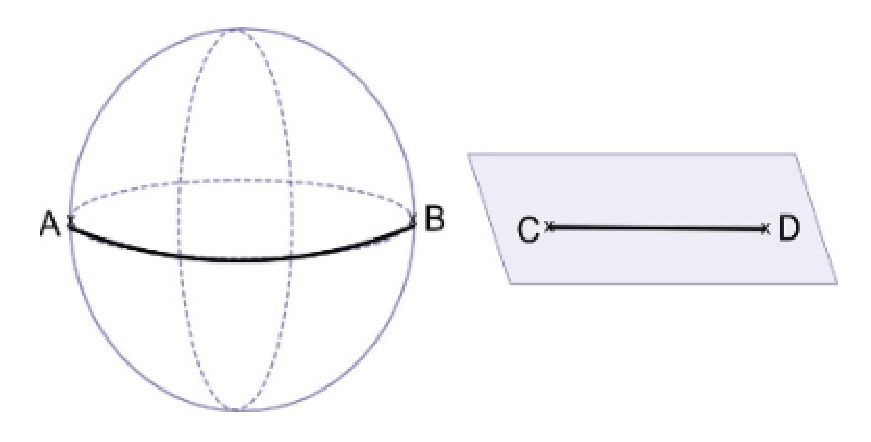
\includegraphics[scale=0.35]{fig12_1.eps}
	\figcaption{弯曲空间与平直空间中的两点间距}
    \label{fig12.1}
}

现在就能“导出” Einstein 场方程了,因为能放在能动张量对面的量只有一个:Einstein张量$G_{\mu \nu}$。这是因为 Einstein 张量是度规$g_{\mu \nu}$及其一阶、二阶导数的函数中唯一\footnote{译注:至多差一常数与度规张量的乘积,即著名的宇宙学常数$Lambda$} 的无散度%
\mpar{即$\partial^\mu G_{\mu \nu} = 0$.}%
函数。不管其多复杂,放到等号一边描述曲率的量只能是它,因为
\begin{equation}
\label{equ12.3}
    T_{\mu \nu} = C G_{\mu \nu}, \quad \text{由} \partial^\mu T_{\mu \nu} = 0 \to \partial^\mu G_{\mu \nu} = 0.
\end{equation}
Einstein 张量是二阶张量%
\mpar{二阶张量是指它有两个指标$\mu \nu$,这与散度为零一样也是限制之一,因为$T_{\mu \nu}$是二阶张量。}%
,正好符合要求。

Einstein张量通过Ricci张量$R_{\mu \nu}$、Ricci标量$R$(即Ricci张量的迹:$R \equiv R^\nu_\nu$)和度规张量$g_{\mu \nu}$定义:
\begin{equation}
\label{equ12.4}
    G_{\mu \nu} = R_{\mu \nu} - \frac{1}{2} R g_{\mu \nu}.
\end{equation}
其中Ricci张量由Christoffel符号$\Gamma^\mu_{\nu \rho}$定义:
\begin{equation}
\label{equ12.5}
    R_{\alpha \beta} = \partial_\rho \Gamma^\rho_{\beta \alpha} - \partial_\beta \Gamma^\rho_{\rho \alpha} + \Gamma^\rho_{\rho \lambda} \Gamma^\lambda_{\beta \alpha} - \Gamma^\rho_{\beta \lambda} \Gamma^\lambda_{\rho \alpha}
\end{equation}
其中 Christoffel 符号通过度规张量定义:
\begin{equation}
\label{equ12.6}
    \Gamma^d_{ab} = \frac{1}{2} g^{cd} \left( \frac{\partial g_{ca}}{\partial x^b} + \frac{\partial g_{cb}}{\partial x^a} - \frac{\partial g_{ab}}{\partial x^c} \right) = \frac{1}{2} g^{cd} (\partial_b g_{ca} + \partial_a g_{cb} - \partial_c g_{ab}).
\end{equation}
上面的式子复杂得吓人,这稍微揭示了广义相对论计算的繁复程度。

现在考虑物体在弯曲时空中的行为。设自由物体经过弯曲时空中的$A, B$两点,物体在$A, B$之间的轨迹是怎样的?容易猜想物体沿弯曲时空中两点间的最短路径(称为短程线)运动,确实如此(证明略)。这样,给定质能分布$T_{\mu \nu}$之后就可根据Einstein场方程计算度规与Christoffel符号,从而得到自由质点的轨迹——{\bf 短程线方程(geodesic equation)}:
\begin{equation}
\label{equ12.7}
    \frac{d^2 x^\lambda}{dt^2} + \Gamma^\lambda_{\mu \nu} \frac{d x^\mu}{dt} \frac{d x^\nu}{dt} = 0.
\end{equation}
测地线是流形上的两点间局域最短%
\mpar{这一说法是过于简单的,正确的概念需要微分几何的相关知识,超出本书范围。}%
的连线。

有趣的是,Einstein将Christoffel符号视作引力场%
\mpar{一般将度规视为引力场。}%
:
\begin{quote}
若$\Gamma^\mu_{\nu \rho}$消失,则(自由)质点沿直线匀速运动,因此$\Gamma^\mu_{\nu \rho}$描述了关于匀速直线的偏离,它们是引力场的分量。
\end{quote}
\begin{flushright}
-- {\bf Albert Einstein}\mpar{Albert Einstein. The foundation of the general theory of relativity. 1916}
\end{flushright}
从\ref{equ12.7}式就能理解Einstein所说的,令$\Gamma^\mu_{\nu \rho} = 0$,测地线方程退化为:
\begin{equation}
\label{equ12.8}
    \frac{d^2 x^\lambda}{dt^2} = 0.
\end{equation}
方程的解是一条直线。

弯曲时空的另一有趣事实是微分符号的变化。平直时空中的导数利用下式定义:
\begin{equation}
\label{equ12.9}
    f'(a) = \lim_{h \to 0} \frac{f(a + h) - f(a)}{h}.
\end{equation}
上式用到了函数$f$在两个不同点的值。弯曲时空的情形不像平直时空那样简单。如图12.2,如果想比较球面上不同位置的两个向量的差值,怎样才能得到它们真正的差而除去弯曲空间造成的影响?微分几何告诉我们可以进行平移,将一个向量平移到另一个向量的位置,从而可以%
\mpar{实际上,微分几何中的坐标系都是局域的。\ref{sec3.11}节讲过,流形的主要特征是局域平直(像Euclidean空间)。因此,流形上对象的坐标只在一个坐标域内有效,同样只能在同一坐标域内比较不同对象的坐标差值。}%
比较它们。

\marginpar{
	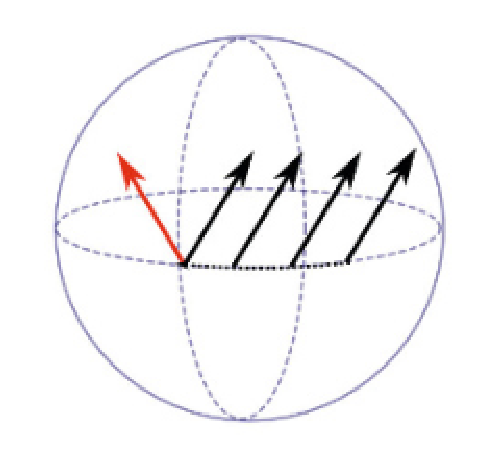
\includegraphics[scale=0.5]{fig12_2.eps}
	\figcaption{为了比较红色箭头与黑色箭头,我们将黑色箭头平移到红色箭头的位置。}
}

弯曲空间中的导数称为{\bf 协变导数 (covariant derivative)}%
\mpar{这里的Christoffel符号$\Gamma^a_{\phantom{a}bc}$通常称为联络系数,因为它们联系了进行比较的两点。}%
:
\begin{equation}
\label{equ12.10}
    D_b v^a \equiv \partial_b v^a + \Gamma^a_{\phantom{a}bc} v^c.
\end{equation}
因此,弯曲时空中的方程需要将普通导数替换为协变导数:
\begin{equation}
\label{equ12.11}
    \partial_b \to D_b = \partial_b + \Gamma^a_{\phantom{a}bc}.
\end{equation}
这很眼熟。见\ref{equ7.18}式,我们在先前的章节中讲过,自旋$0$或自旋$\frac{1}{2}$场拉格朗日量的局域$\mathcal{U}(1)$不变性要求与自旋$1$的场有特定的耦合。这一耦合可以用下式描述:
\begin{equation}
\label{equ12.12}
    \partial_\mu \to D_\mu \equiv \partial_\mu + i \mathrm{e} A_\mu.
\end{equation}
注意这不只是个数学技巧,它导出了正确的电磁学理论。弱相互作用的情形也类似:
\begin{equation}
\label{equ12.13}
    \partial_\mu \to D_\mu \equiv \partial_\mu + i g \underbrace{W_\mu}_{\mathclap{= W_\mu^i \sigma^i}}.
\end{equation}
强相互作用也是:
\begin{equation}
\label{equ12.14}
    \partial_\mu \to D_\mu = \partial_\mu + i g' \underbrace{G_\mu}_{\mathclap{= T^C G^C_\mu}}.
\end{equation}
尽管上面各式的形式相似,但引力无法像其他相互作用那样量子化。其他相互作用都是用量子理论描述的,都给出概率性的实验预言。而广义相对论是经典理论,因为广相中的粒子沿确定的轨迹运动,没有概率性因素。

更糟糕的是目前没有任何实验能检测引力与其他力之间的相互作用。基本粒子间的引力太小,无法测量。因此忽视了引力,只考虑强、弱与电磁相互作用的标准模型就可以与实验符合得相当好。大质量物体的广义相对论效应实验上可以测量,但量子效应却十分微弱,因为大质量物体包含大量基本粒子,所有量子效应被平均掉了。第\ref{chap10}章导出了平均值的运动方程,它正是经典物理的形式,毫无量子效应。

引力的量子化的困难可以列出长长的列表,不过Einstein简明地论述了引力与其他相互作用的差异:
\begin{quote}
$\dots$ 根据广义相对论,引力与其他相互作用(特别是电磁力)相比地位特殊,因为描述引力场的十个方程\footnote{或许指Einstein场方程,代表十个方程。——译者}同时确定了时空的度量性质。
\end{quote}
\begin{flushright}
-- {\bf Albert Einstein}\mpar{Albert Einstein and Francis A. Davis.
{\it The Principle of Relativity}. Dover Publications, reprint edition, 6 1952. ISBN 9780486600819}
\end{flushright}

将普通导数替换为协变导数就能描述弯曲时空中的量子粒子,但这并非引力的动力学理论。Einstein场方程等号右侧(能动张量)容易量子化,选定合适的生成元就行了。困难的是等号左边的Einstein张量,它用Christoffel符号写为:
\begin{equation}
\label{equ12.15}
    G_{\alpha \beta} = (\delta^\gamma_\alpha \delta^\zeta_\beta - \frac{1}{2} g_{\alpha \beta} g^{\gamma \zeta}) (\partial_\varepsilon \Gamma^\varepsilon_{\gamma \zeta} - \partial_\zeta \Gamma^\varepsilon_{\gamma \varepsilon} + \Gamma^\varepsilon_{\varepsilon \sigma} \Gamma^\sigma_{\gamma \zeta} - \Gamma^\varepsilon_{\zeta \sigma} \Gamma^\sigma_{\varepsilon \gamma}).
\end{equation}
由此猜想Einstein场方程或许是$\Gamma^\varepsilon_{\zeta \sigma}$的场方程%
\mpar{就像Maxwell方程组与电磁场的关系那样。}%
,并且$\partial_b \to D_b = \partial_b + \Gamma^a_{\phantom{a} bc}$描述引力场$\Gamma^\varepsilon_{\zeta \sigma}$与其他场的耦合。

无论将度规张量(两个指标)还是Christoffel符号(三个指标)视为引力场,描述它们都需要Poincare群的$(1, 1)$以及更高维的表示,或者说自旋$2, 3, \dots$表示。目前大多数物理学家认为引力场量子化后的引力子(graviton)是自旋为$2$的boson。

目前为止,没有靠谱的量子引力理论%
\mpar{许多尝试过程产生了无穷多个无穷大项,这对概率性预言来说十分要命。}%
能比下一节列出教科书上的标准引力理论给出进一步的信息。

\section*{Further Reading Tips \quad 阅读建议}
引力的标准理论——Einstein的广义相对论的更多信息可以参考以下文献:
\begin{itemize}
    \item {\bf  Ta-Pei Cheng - Relativity, Gravitation and Cosmology}%
    \mpar{Ta-Pei Cheng. {\it Relativity, Gravitation and Cosmology: A Basic Introduction.} Oxford University Press, 2nd edition, 1. 2010. ISBN 9780199573646}%
    是一本内容丰富、起点低的广义相对论入门教材,其中有大量启发性的论述。是快速入门的首选。
    \item {\bf  A. Zee - Einstein Gravity in a Nutshell}%
    \mpar{Anthony Zee. {\it Einstein Gravity in a Nutshell.} Princeton University Press, 1st edition, 5. 2013. ISBN 9780691145587}%
    是广义相对论的最佳教材。此书从基本概念开始,避免不必要而复杂的数学概念,精彩地解释了广义相对论的起源与应用。
    \item {\bf  Charles W. Misner, Kip S. Thorne, John Archibald Wheeler - Gravitation}%
    \mpar{ Charles W. Misner, Kip S. Thorne, and John Archibald Wheeler. {\it Gravitation.} W.H. Freeman, 1st edition, 9. 1973. ISBN 9780716703440}%
    是一本关于引力的鸿篇巨著,其中阐明了有大量其他教材未深入讨论的问题。
\end{itemize}
关于尝试引力量子化的更多信息可见
\begin{itemize}
    \item {\bf John C. Baez, Javier P. Muniain - Gauge Fields, Knots, and Gravity}%
    \mpar{ John C. Baez and Javier P. Muniain. {\it Gauge Fields, Knots, and Gravity.} World Scientific Pub Co Inc, 1st edition, 9. 1994. ISBN 9789810220341}%
    以面向物理学家的方式介绍了引力量子化的数学工具。
\end{itemize}

%!TEX root = ..\main.tex
%!TEX encoding = UTF-8 Unicode

%——————————————————————————————————————————————————————————-
%	CHAPTER 13
%   Translator:SI
%   Proofread : lh1962
%——————————————————————————————————————————————————————————-
\chapterimage{chapter_head_1.pdf} % Chapter heading image

\chapter{结束语}
\label{chap13}
在我看来,目前人类距离描述万物的万有理论还十分遥远。即使是本书主体部分所描述的优美理论也还存在着许多有待阐明的地方\footnote{比如本书多得要命的typo,赶快出修订版吧!——译者}。此外,如上一章所述,量子引力理论仍一筹莫展。

而且现在存在着实验证据(主要是宇宙学与天体粒子物理学的暗物质与暗能量疑难)表明现有理论仍有待改进。

我个人觉得现有疑难的背后仍蕴藏着大量内容,甚至或许是物理学的崭新框架。无论如何,未来的进展都非常有趣,衷心祝愿你会沿着这条路走向更远。

\appendix

%!TEX root = main.tex
%!TEX encoding = UTF-8 Unicode

\appendix
\part{Appendix 附录}
\chapter[矢量代数]{Vector calculus 矢量代数}\label{appendix.A}
物理中常用三个数$ \begin{pmatrix}
x \\ y \\ z
\end{pmatrix}$来描述一个东西的位置。我们将其称作矢量$\vec{v}$,在它头上放了一个箭头。这三个数称作矢量沿三个坐标轴的分量。第一个数说了这个矢量沿$x$方向走了多远,第二个是沿$y$方向以及第三个是沿$z$方向。例如,$\vec{w}= \begin{pmatrix}
0 \\ 4 \\ 0
\end{pmatrix}$是一个指向$y$轴方向的矢量。

\marginpar{
	\includegraphics[width=.4\textwidth]{Figure/fig_appendix_A_1.png}
}

矢量间可以相加
\begin{equation}
\vec{v} = \begin{pmatrix}
v_x \\ v_y \\ v_z
\end{pmatrix} \quad
\vec{w} = \begin{pmatrix}
w_x \\ w_y \\ w_z
\end{pmatrix} \quad \rightarrow \quad
\vec{v}+\vec{w}= \begin{pmatrix}
v_x+w_x \\ v_y+w_y \\ v_z+w_z
\end{pmatrix}
\end{equation}
也可以相乘
\begin{equation}
\vec{v}\cdot\vec{w} = \begin{pmatrix}
v_x \\ v_y \\ v_z
\end{pmatrix} \cdot \begin{pmatrix}
w_x \\ w_y \\ w_z
\end{pmatrix} =
v_xw_x +v_yw_y +v_zw_z\text{。}
\end{equation}

乘法的结果是一个数($=$标量)而不是矢量,其有特定的名称:{标量积(scalar product)}。计算矢量与自身的标量积可以得到其长度:
\begin{equation}
\text{长度}(\vec{v}) = \sqrt{\vec{v}\cdot\vec{v}}\text{。}
\end{equation}
注意并不是随便三个量都可以写在一起,用括号包起来,作为一个矢量。例如,把一个房间里的温度$T$,压强$P$和湿度$H$放在一起:
\begin{equation}
\begin{pmatrix}
T \\ P \\ H
\end{pmatrix}\text{。}
\end{equation}
没人阻止我们把他们放在一起,但这结果毫无意义,而且显然不是一个矢量,因为不存在能将它们混在一起的线性关系。而如果我们仅仅是换一个视角\footnote{译注:本意,即视线的角度。}去考察一个矢量,它的坐标分量将会互相转换%
\mpar{这一点等会儿会有更清楚的说明。}%
。故将这些坐标分量写在一起用括号包起来是有用的。另外,如果分量会因视角的改变而发生混合的话,将其写成位置矢量的形式是有用的。

从现在开始,我们将完全按照位置矢量$\vec{v}$的变换方式的量称为一个矢量。这句话的意思是,如果在某种变换下我们有$\vec{v}\rightarrow\vec{v}'=M\vec{v}$,则任何依$\vec{w}\rightarrow\vec{w}'=M\vec{w}$作变换的量都是矢量。动量和加速度是典型的例子。

物理中我们将经常碰到这种思路。当我们把一些量写在一起放在一对括号中时,它们未必是矢量,但一定是在某些线性算符下相互变换的量。线性算符常通过与矩阵的乘法来表示。

\section[基矢]{Basis Vectors 基矢}\label{appendix.A.1}
我们可以通过引入基矢来更一般的讨论沿坐标轴的分量这件事。基矢是一组线性独立%
\mpar{一组矢量$\{\vec{a},\vec{b},\vec{c}\}$被称为是线性独立的,若方程$c_1\vec{a}+c_2\vec{b}+c_3\vec{c}=0$成立当且仅当$c_1=c_2=c_3=0$。这说的其实就是其中任何一个矢量不能表达为其他矢量的线性组合:如果有$c_1\vec{a}+c_2\vec{b}+c_3\vec{c}=0$对非零的系数成立,则有$c_1\vec{a}+c_2\vec{b}=-c_3\vec{c}$。}%
且长度为一%
\footnote{译注:一般资料上并不要求最后一条;满足这一条的称为单位基矢。}%
的矢量。三维里我们需要三个基矢,从而能将任何矢量都用基矢量的组合来表达。一个简单的选择是:
\begin{equation}
\vec{e}_1 = \begin{pmatrix}
1 \\ 0 \\ 0
\end{pmatrix}\text{,}\quad
\vec{e}_2 = \begin{pmatrix}
0 \\ 1 \\ 0
\end{pmatrix} \text{,}\quad
\vec{e}_3 = \begin{pmatrix}
0 \\ 0 \\ 1
\end{pmatrix}
\end{equation}
这样任意三维矢量$\vec{v}$都能用基矢表出
\begin{equation}
\vec{v} = \begin{pmatrix}
v_x \\ v_y \\ v_z
\end{pmatrix} = v_1\vec{e}_1 + v_2\vec{e}_2 + v_3\vec{e}_3 =
v_1 \begin{pmatrix}
1 \\ 0 \\ 0
\end{pmatrix}+
v_2  \begin{pmatrix}
0 \\ 1 \\ 0
\end{pmatrix} +
v_3  \begin{pmatrix}
0 \\ 0 \\ 1
\end{pmatrix}\text{。}
\end{equation}
$v_1,v_2,v_3$三个数叫做$\vec{v}$的分量。注意分量是依赖于基矢的。

前面提到的矢量\mpar{$\vec{w}= \begin{pmatrix}
0\\4\\0
\end{pmatrix}$}$\vec{w}$由此可以写成$\vec{w}= 0\vec{e}_1 + 4\vec{e}_2 + 0\vec{e}_3$。对基矢另一个同样好的选法是
\begin{equation}
\tilde\vec{e}_1 = \frac{1}{\sqrt{2}} \begin{pmatrix}
1 \\ 1 \\ 0
\end{pmatrix}\text{,}\quad
\tilde\vec{e}_2 = \frac{1}{\sqrt{2}} \begin{pmatrix}
1 \\ -1 \\ 0
\end{pmatrix} \text{,}\quad
\tilde\vec{e}_3 = \begin{pmatrix}
0 \\ 0 \\ 1
\end{pmatrix}\text{。}
\end{equation}
在这组基下矢量$\vec{w}$看起来会有点不同:
\begin{equation}
\vec{w}= 2\sqrt{2}\tilde\vec{e}_1 -2\sqrt{2}\tilde\vec{e}_2 + 0\tilde\vec{e}_3
= 2\sqrt{2} \frac{1}{\sqrt{2}} \begin{pmatrix}
1 \\ 1 \\ 0
\end{pmatrix}-2\sqrt{2}
\frac{1}{\sqrt{2}} \begin{pmatrix}
1 \\ -1 \\ 0
\end{pmatrix} =\begin{pmatrix}
0\\4\\0
\end{pmatrix} \text{。}
\end{equation}
从而将$\vec{w}$用在新基矢下的分量写出
\[
\tilde\vec{w} = \begin{pmatrix}
2\sqrt{2} \\ -2\sqrt{2} \\ 0
\end{pmatrix}\text{。}
\]
这并不是一个不同的矢量,而只是一个不同的描述!准确地讲,$\tilde\vec{w}$是原坐标系中的矢量$\tilde\vec{w}$在一个相对有旋转的坐标系下描述。%
\footnote{译注:在整个附录\ref{appendix.A}里作者就没说过几句准确的话,这句话也说得挺糙的。}

\section[坐标系变换]{Change of Coordinate Systems 坐标系变换}\label{appendix.A.2}
通过矩阵,我们可以更精确地描述不同坐标系间的联系。两个不同的坐标系可以代表实验中两个持不同视角的观察者,或者仅仅是{\bf 一个}想使用一套新的基矢的观察者。这些描述之间的关系是什么?为了避免复杂的讨论,让我们假定这两个坐标系的原点和$z$轴都是一样的。这样的话就只是$x$和$y$轴有区别了。进一步假定实验中某个重要的量用矢量$\vec{v}$描述。

如果第一个观察者看到的是矢量$\vec{v}= \begin{pmatrix}
v_x \\ v_y \\ v_z
\end{pmatrix}$,我们能通过三角函数$\sin(\phi)$,$\cos(\phi)$和$\tan(\phi)=\frac{\sin(\phi)}{\cos(\phi)}$来计算出第二个观察者看到的$\vec{v}= \begin{pmatrix}
v_{x'} \\ v_{y'} \\ v_{z'}
\end{pmatrix}$,如图\ref{fig:appendix.A.1} 所示:
\marginpar{
	\figcaption{矢量在两个不同的坐标系下分量的示意图。细节见正文。}
	\label{fig:appendix.A.1}
}

\includegraphics[width=\textwidth]{Figure/fig_appendix_A_3.png}

计算$v_x$和$v_{x'}$的关系,由
\[
\cos(\phi)=\frac{v_{x'}}{v_x+a} \rightarrow v_{x'}=(v_x+a)\cos(\phi)
\]
以及
\[
\tan(\phi)=\frac{a}{v_y}\rightarrow a=v_y\tan(\phi)\text{。}
\]
得到
\[
\begin{aligned}
v_{x'}=(v_x+v_y\tan(\phi))\cos(\phi)&=\left(v_x+v_y\frac{\sin(\phi)}{\cos(\phi)}\right)\cos(\phi) \\
 & = v_x\cos(\phi)+v_y\sin(\phi)\text{。}
\end{aligned}
\]
类似的,利用
\[
\cos(\phi) = \frac{v_y}{v_{y'}+b}\rightarrow v_{y'}=v_y\frac{1}{\cos(\phi)}-b
\]
和
\[
\tan(\phi)=\frac{v_y}{v_{y'}+b}\rightarrow b=v_{x'}\tan(\phi)
\]
再借助$\sin^2(\phi)+\cos^2(\phi)=1$导出
\[
\begin{align}
v_{y'}&=v_y\frac{1}{\cos(\phi)}-v_{x'}\tan(\phi)=v_y\frac{1}{\cos(\phi)}-(v_x\cos(\phi)+v_y\sin(\phi))\frac{\sin(\phi)}{\cos(\phi)}  \\
&= v_y\frac{\sin^2(\phi)+\cos^2(\phi)}{\cos(\phi)}-v_x\sin(\phi)-v_y\frac{\sin^2(\phi)}{\cos(\phi)} = v_y\cos(\phi)-v_x\sin(\phi)
\end{align}
\]
最终有$v_{y'}=-v_x\sin(\phi)+v_y\cos(\phi)$。

我们能将其用一个旋转矩阵来表达:
\begin{equation}
\begin{aligned}
\begin{pmatrix}
v_{x'} \\ v_{y'} \\ v_{z'}
\end{pmatrix} &= R_z(\phi)\vec{v} =
\begin{pmatrix}
\cos(\phi) & \sin(\phi) & 0 \\
-\sin(\phi) & \cos(\phi) & 0 \\
0 & 0 & 1
\end{pmatrix}
\begin{pmatrix}
v_x \\ v_y \\ v_z
\end{pmatrix} \\
&= \begin{pmatrix}
\cos(\phi)v_x+\sin(\phi)v_y \\ -\sin(\phi)v_x+\cos(\phi)v_y \\ v_z
\end{pmatrix}\text{。}
\end{aligned}
\end{equation}
将矩阵的每一行与未旋转的矢量相乘,便得到了旋转后的矢量。如之前所提到的,沿$z$轴的分量$v_3$对于不同的观察者而言是相同的。矩阵$R_z(\phi)$描述了一个绕$z$轴转动了角度$\phi$的旋转。

\section[矩阵乘法]{Matrix Multiplication 矩阵乘法}\label{appendix.A.3}
像这样通过矩阵来作计算是一个极大的简化。矩阵乘法的规则就是行乘列。如果将一个矢量看做一个一列三行的矩阵(一个$3\times 1$矩阵),则标量积也可以看做是矩阵乘法的一种特殊情况。即
\begin{equation}
\vec{v}\cdot\vec{w} = \vec{v}^T\vec{w}= \begin{pmatrix}
v_x & v_y & v_z
\end{pmatrix} \begin{pmatrix}
w_x \\ w_y \\ w_z
\end{pmatrix} = v_xw_x +v_yw_y +v_zw_z\text{,}
\end{equation}
其中$T$代表转置,即行变成列,列变成行。那么$\vec{v}^T$便是一个$1$行$3$列的矩阵。这样写的话标量积就也成了行乘列的矩阵乘法。

类似的,两个矩阵的乘法也就是左边矩阵的每一行乘右边矩阵的每一列,如图\ref{fig:appendix.A.2}。下面是一个具体的例子

\marginpar{
	\includegraphics[width=.4\textwidth]{Figure/fig_appendix_A_4.png}
	\figcaption{矩阵乘法示意图。时时刻刻记住{\bf 行乘列}。第一个指标代表所在的行数,第二个代表列数。在例子中,乘积矩阵红色的元素$c_{1,2}=a_{1,1}b_{1,2}+a_{1,2}b_{2,2}$,蓝色的元素$c_{3,3}=a_{3,1}b_{1,3}+a_{3,2}b_{2,3}$。一般的,$c_{i,j}=a_{i,k}b_{k,j}=a_{i,1}b_{1,j}+a_{i,2}b_{2,j}+\dots$ Figure by Olivier Perrin (Bilou Wikimedia Commons) released under a CC BY-SA 3.0 licence: \url{http://creativecommons.org/licenses/by-sa/3.0/deed.en}. URL: \url{http://commons.wikimedia.org/wiki/File:Matrix_multiplication_diagram_2.svg}, Accessed: 28.1.2015}
	\label{fig:appendix.A.2}
}

\begin{equation}
\begin{aligned}
M= \begin{pmatrix}
2 & 3 \\ 1 & 0
\end{pmatrix} \quad N =
\begin{pmatrix}
0 & 1 \\ 4 & 8
\end{pmatrix} \\
MN = \begin{pmatrix}
2 & 3 \\ 1 & 0
\end{pmatrix}
\begin{pmatrix}
0 & 1 \\ 4 & 8
\end{pmatrix} =
\begin{pmatrix}
2\cdot 0+3\cdot 4 & 2\cdot 1+3\cdot 8 \\ 1\cdot 0+0\cdot 4 & 1\cdot 1+0\cdot 8
\end{pmatrix} =
\begin{pmatrix}
12 & 26 \\ 0 & 1
\end{pmatrix}
\end{aligned}
\end{equation}
时刻把{\bf 行乘列}记在脑子里\footnote{译注:说起来,什么是行什么是列也是一个需要记牢的东西,尤其是与台湾友人交流时。}。注意两个矩阵的乘法是不对易的,即一般来说$MN\ne NM$。

\section[标量]{Scalars 标量}\label{appendix.A.4}
另一个值得注意的事情是,两个矢量标量积的结果对于所有观察者而言都是相同的。这看起来可以作为标量的定义:标量是对于全部观察者都相同的量。这不只是简单的在说每一个数都是标量,因为矢量的每一个分量都是一个数,但是它们对于不同的观察者而言却不一样。作为对比,两个矢量的标量积对于全体观察者却是相同的。这源于,矢量的长度与其与自身的标量积直接相关这一事实。改变观察的视角或位置并不会改变任何东西的长度。矢量的长度被称作旋转下的不变量,即无论我们怎样旋转系统其都保持原样。

\section[左手/右手坐标系]{Right-handed and Left-handed Coordinate Systems 左手/右手坐标系}\label{appendix.A.5}
当我们谈论两个观察者时,我们默认了它们对坐标系的定义都是相同的。而事实上,我们有两种可能的选择,它们这是依旧能通过矩阵乘法相联系,却不能靠转动了。两个观察者可能是一个选择了所谓的右手坐标系,而另一个选择了左手坐标系。

\marginpar{
	\includegraphics[width=.4\textwidth]{Figure/fig_appendix_A_5.png}
	\figcaption{右手坐标系和左手坐标系。 Figure by Primalshell (Wikimedia Commons) released under a CC-BY-SA-3.0 licence: \url{http://creativecommons.org/licenses/by-sa/3.0/deed.en}. URL:\url{http://commons.wikimedia.org/wiki/File:3D_Cartesian_Coodinate_Handedness.jpg}, Accessed: 1.12.2014}
}

我们无法将一个左手系旋转成一个右手系。事实上,这两类坐标系通过镜面反射相关联。这就是说,右手系和左手系由如下形式的变换相联系%
\footnote{译注:原文这里给出的其实是一个相对原点的反射,而不是镜面反射。当然,这两种反射之间只差一个转动。}
\begin{equation}
\begin{pmatrix}
v_1 \\ v_2 \\ v_3
\end{pmatrix} \rightarrow
\begin{pmatrix}
-v_1 \\ -v_2 \\ -v_3
\end{pmatrix}\text{,}
\end{equation}
就是说把全部空间坐标都反一个号。人们也习惯于将这类变换称作{\bf 宇称变换(parity transformation)}。我们可以用如下方式来表示一个宇称变换
\begin{equation}
\vec{v} \rightarrow \vec{v}' = P\vec{v} = \begin{pmatrix}
-1 & 0 & 0 \\ 0 & -1 & 0 \\ 0 & 0 & -1
\end{pmatrix}
\begin{pmatrix}
v_1 \\ v_2 \\ v_3
\end{pmatrix} =
\begin{pmatrix}
-v_1 \\ -v_2 \\ -v_3
\end{pmatrix}\text{。}
\end{equation}

\chapter[微积分]{Calulus 微积分}

\section[Product Rule]{Product Rule 莱布尼兹律}

\section[分部积分]{Integration by Parts 分部积分}

\section[Taylor 级数]{The Taylor Series\quad Taylor 级数}

\section[级数]{Series 级数}
\subsection[几个重要的级数]{Important Series 几个重要的级数}
\subsection[分裂求和]{Splitting Sums 分裂求和}
\subsection[Einstein 求和约定]{Einstein’s Sum Convention\quad Einstein 求和约定}

\section[指标记号]{Index Notation 指标记号}
\subsection[哑指标]{Dummy Indices 哑指标}
\subsection[带多个指标的对象]{Objects with more than One Index 带多个指标的对象}
\subsection[对称/反对称指标]{Symmetric and Antisymmetric Indices 对称/反对称指标}
\subsection[对称和反对称求和]{Antisymmetric $\times$ Symmetric Sums 对称和反对称求和}
\subsection[两个重要的符号]{Two Important Symbols 两个重要的符号}

\chapter[线性代数]{Linear Algebra 线性代数}
\section[基本的变换]{Basic Transformations 基本的变换}
\section[矩阵指数函数]{Matrix Exponential Function 矩阵指数函数}
\section[行列式]{Determinants 行列式}
\section[本征值与本征向量]{Eigenvalues and Eigenvectors 本征值与本征向量}
\section[对角化]{Diagonalization 对角化}

\chapter[其他数学概念]{Additional Mathematical
Notions 其他数学概念}
\section[Fourier 变换]{Fourier Transform\quad Fourier 变换}
\section[Delta 分布]{Delta Distribution\quad Delta 分布}


\backmatter

%----------------------------------------------------------------------------------------
%	BIBLIOGRAPHY
%----------------------------------------------------------------------------------------

%\cleardoublepage
%\bibliographystyle{apsrev4-1}
%\bibliography{bibliography}

%----------------------------------------------------------------------------------------
%	INDEX
%----------------------------------------------------------------------------------------

%\cleardoublepage
%\phantomsection
%\setlength{\columnsep}{0.75cm}
%\addcontentsline{toc}{chapter}{\textcolor{ocre}{Index}}
%\printindex



\end{document}
